\documentclass[12pt,a4paper]{report}

% --- Encoding and language ---
\usepackage[utf8]{inputenc}
\usepackage[T1]{fontenc}
\usepackage[english]{babel}

% --- Font (Lato: modern sans-serif, PDFLaTeX-compatible) ---
\usepackage[scaled=0.95]{helvet}
\renewcommand{\familydefault}{\sfdefault}

% --- Page layout ---
\usepackage[a4paper,margin=2.5cm]{geometry}
\usepackage{setspace}
\onehalfspacing

\usepackage{graphicx}

% --- For subsections ---
\setcounter{tocdepth}{3}
\setcounter{secnumdepth}{3}
\usepackage{titlesec}

% --- Chapter format: "1. Title" ---
\titleformat{\chapter}[hang]
{\normalfont\Large\bfseries}
{\thechapter.}
{0.6em}
{}

\usepackage{xcolor}
\usepackage{tabularx}
\usepackage{array}
\usepackage{booktabs}
\usepackage{colortbl}

% --- Colours for the summary tables (chapter status) ---
\definecolor{codegreen}{RGB}{76,175,80}
\definecolor{warningyellow}{RGB}{255,193,7}

\usepackage{placeins}
\usepackage{float}

\usepackage{enumitem}
\usepackage{amsmath}

\usepackage{listings}
\usepackage{rotating}

% --- Style for displaying Python source code ---
\lstdefinestyle{pythonstyle}{
	language=Python,
	backgroundcolor=\color{gray!5},
	basicstyle=\ttfamily\footnotesize,
	keywordstyle=\color{blue}\bfseries,
	stringstyle=\color{codegreen},
	commentstyle=\color{gray}\itshape,
	numbers=left,
	numberstyle=\tiny\color{gray},
	stepnumber=1,
	numbersep=8pt,
	frame=single,
	breaklines=true,
	showstringspaces=false,
	tabsize=4,
	captionpos=b
}
\lstset{style=pythonstyle}

\usepackage[hidelinks]{hyperref}


\setlength{\emergencystretch}{3em}
\begin{document}
\begin{titlepage}
	\centering
	\vspace*{1cm}
	{\huge\bfseries Gesture-Controlled IOT Car:\\[4pt] Benchmark of Five Embedded Vision Solutions \par}
	\vspace{0.6cm}
	{\large\itshape Technical benchmark report - methodology, measurements and analysis \par}
	\vspace{1.2cm}
	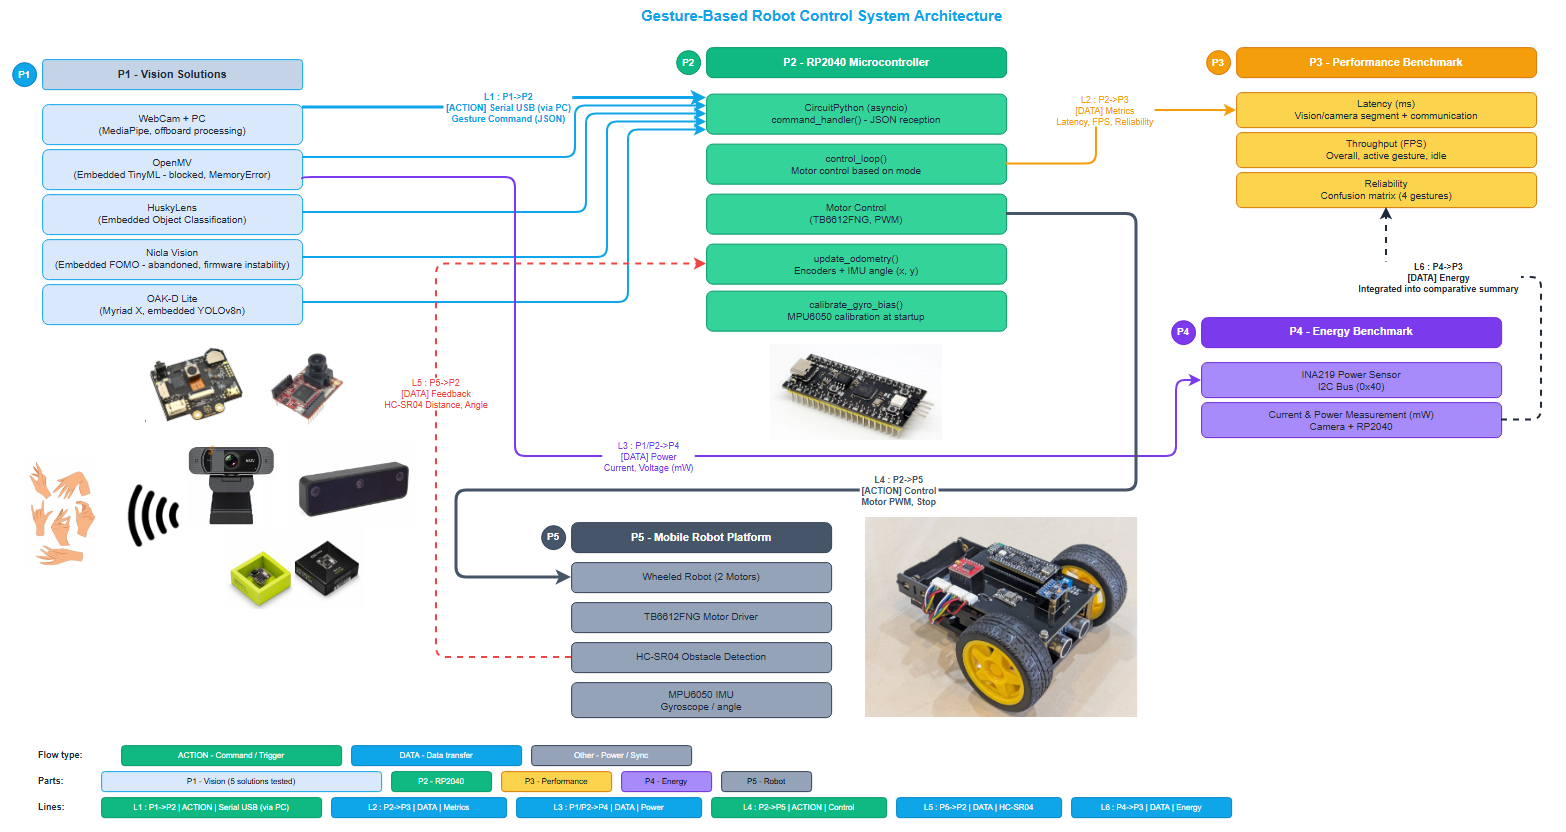
\includegraphics[width=0.85\linewidth]{Architecture_Systeme_Benchmark.png}
	\vfill
	{\large
		Sivaharan KUMARA SEGARAM \\[2pt]
		R\&D internship - Academic project abroad (Taiwan) \\[2pt]
		Embedded Systems \quad - \quad May to July 2026
		\par}
	\vspace{0.8cm}
	{\small\itshape Extracted and condensed from the full internship report (written in French, translated into English), keeping only the benchmark.\par}
\end{titlepage}
\pagenumbering{roman}
\chapter*{Summary}
\addcontentsline{toc}{chapter}{Summary}
Five camera solutions were integrated into the same gesture-control chain and compared on identical metrics:
a generic webcam with MediaPipe, the OpenMV Cam M7, the Arduino Nicla Vision, the DFRobot HuskyLens and the Luxonis OAK-D Lite (YOLOv8n).
Each camera recognises four hand gestures (forward, stop, left, right); a PC relays the command over USB/UART (JSON) to an RP2040-based robot (IOT Car).
To keep the communication segment a controlled variable, every solution goes through the same PC relay, even the cameras able to work autonomously.

\medskip
\begin{center}
\small
\renewcommand{\arraystretch}{1.25}
\begin{tabularx}{\linewidth}{>{\raggedright\arraybackslash}p{4.0cm}*{4}{>{\centering\arraybackslash}X}}
\toprule
\textbf{Solution} & \textbf{Total latency (median)} & \textbf{Throughput (median)} & \textbf{Reliability (80 trials)} & \textbf{Power} \\
\midrule
WebCam + MediaPipe & 29.82 ms & 31.62 FPS & 100.0\,\% & not measured \\
OpenMV Cam M7 & \multicolumn{4}{c}{\textit{not measurable (the model does not fit in RAM)}} \\
Nicla Vision & 68.78 ms & 12.82 FPS & 83.8\,\% & not measured \\
HuskyLens & 5.85 ms & 492.08 FPS & 86.2\,\% & not measured \\
OAK-D Lite & 50.51 ms & 31.98 FPS & 72.5\,\% & not measured \\
\bottomrule
\end{tabularx}
\end{center}
\medskip
No solution dominates on every metric: the HuskyLens is by far the fastest, the webcam is the only one with perfect reliability,
and the OAK-D Lite - the most powerful hardware, with a 96.6\,\% mAP50 at training - is the least reliable in real conditions.
Power consumption could not be measured for any solution (borrowed hardware could not be rewired to insert an INA219 sensor).
\tableofcontents
\newpage
\pagenumbering{arabic}
\setcounter{page}{1}
\chapter{Research question and benchmark design}
	\section{From the initial topic to the benchmark}
	
	\subsection*{Context and new topic}
	
	Faced with the implementation complexity of the complete OpenMV-ESP32-ROS2-Turtlebot~3 chain, and given the availability within the laboratory of an RP2040-based mobile robot platform, the internship topic was reoriented with my supervisor's agreement towards a more experimental problem that was directly achievable within the allotted time:
	
	\begin{quote}
		\itshape Comparative Study of Vision Solutions for the Gesture-Based Control of a Mobile Robot on RP2040: Benchmarking WebCam, OpenMV and HuskyLens. Architecture, Latency, Throughput, Reliability and Power Consumption
	\end{quote}
	
	This new topic aimed to control the robot remotely through hand gesture recognition (move forward, stop, turn left, turn right), while objectively comparing several vision capture and processing architectures: a webcam whose processing (MediaPipe) is entirely offloaded to a PC, and smart cameras embedding their own processing chain (a custom TinyML model or a ready-to-use classification algorithm). The central issue of the project is therefore to determine where to place the processing intelligence in an embedded gesture-control chain, and to objectively measure the trade-offs: latency, throughput, recognition reliability and power consumption.
	
	The initial scope of this reorientation covered three solutions (webcam, OpenMV, HuskyLens). It was extended during the internship to five solutions, following the deployment failure encountered on the OpenMV (Section~\ref{sec:openmv-limitation}) and the recommendations of my supervisor, who suggested adding the Arduino Nicla Vision camera, then the OAK-D Lite stereo camera (Luxonis), in order to enrich the comparison.
	
	\subsection*{State of the art}
	
	Two recent research works form the basis of the state of the art for this project and make it possible to identify the gaps (\textit{research gaps}) that this benchmark seeks to fill.\\
	
	The first work (Bartoli et al., 2025)~\cite{bartoli2025} proposes a benchmarking methodology combining latency and power-consumption measurement for TinyML systems embedded on a microcontroller, with a fine separation of the pre-inference, inference and post-inference phases, validated on an STM32N6 microcontroller equipped with a dedicated NPU.\newline 
	This study is, however, limited to a single hardware platform and a single processing point (always embedded), with no comparison to PC-offloaded processing or to autonomous smart cameras.\\
	
	The second work (Bhushan et al., 2025)~\cite{bhushan2025} presents an object-detection system deployed on an ARM Cortex-M4 microcontroller, combining a camera, a quantised MobileNetV2 model and dual-protocol (TCP/UDP) wireless communication to arbitrate between reliability and low latency.\newline
	This study also relies on a single hardware platform, with no comparison to PC-offloaded processing or ready-to-use smart camera modules, and does not measure recognition reliability by confusion matrix, nor the use case of a mobile robot actually driven by the vision results.\\
	
	These two works therefore share the same limitation: each focuses on a single hardware platform and a single processing point, without ever comparing the different possible distributions of processing intelligence for the same application task. This is precisely the gap that this benchmark project seeks to fill.
	
	\subsection*{Objectives}
	
	The objectives set for this new topic were as follows:
	
	\begin{enumerate}[leftmargin=*]
		\item Define a common, reproducible comparative benchmark protocol, applicable uniformly to the four chosen metrics (latency, throughput, reliability, consumption);
		\item Study and integrate the WebCam solution: gesture detection using a webcam and MediaPipe on a PC, transmission of the commands to the robot over a serial link;
		\item Study and integrate the OpenMV solution: train a custom TinyML model (Edge Impulse) for gesture recognition, deploy it and connect it to the robot;
		\item Study and integrate the HuskyLens solution: train the camera in \textit{Object Classification} mode to recognise the same gestures, and establish the command link to the robot;
		\item Study and integrate the Nicla Vision solution: train a TinyML model (Edge Impulse), following the same methodology as for the OpenMV;
		\item Study and integrate the OAK-D Lite solution: train a YOLOv8n model and deploy it on the camera;
		\item Validate the five solutions on the same robotic platform (IOT Car), over a serial connection;
		\item Measure, for each solution, the latency, the throughput (FPS) and the recognition reliability (confusion matrix);
		\item Measure the power consumption of each camera and of the RP2040, using an INA219 module, at rest and while operating;
		\item Synthesise the comparison of the five solutions across the four metrics, and identify the trade-offs (responsiveness, autonomy, ease of implementation, dependence on a PC);
		\item Document and produce a synthesis report, with the source code available.
	\end{enumerate}
	
	\newpage
	
	\subsection*{Architecture of the gesture-control system}
	
	The final architecture of the system, shown in Figure~\ref{fig:architecture-benchmark}, is organised around five functional blocks:
	
	\begin{itemize}
		\item \textbf{P1 -> Vision solutions (5 solutions tested)}: WebCam~+~PC (MediaPipe, offloaded processing), OpenMV (embedded TinyML, blocked by a memory error), HuskyLens (embedded \textit{Object Classification}), Nicla Vision (embedded FOMO, abandoned due to firmware instability), and OAK-D Lite (Myriad~X, embedded YOLOv8n);
		\item \textbf{P2 -> RP2040 microcontroller}: asynchronous CircuitPython firmware, reception of JSON commands (\texttt{command\_handler()}), motor control according to the active mode (\texttt{control\_loop()}), motor control via TB6612FNG (PWM), odometry from encoders and IMU angle (\texttt{update\_odometry()}), gyroscope bias calibration at startup (\texttt{calibrate\_gyro\_bias()});
		\item \textbf{P3 -> Performance benchmark}: measurement of latency (vision/camera segment and communication segment), throughput (overall FPS, active gesture, neutral) and recognition reliability (confusion matrix over the four gestures);
		\item \textbf{P4 -> Energy benchmark}: INA219 power sensor on the I2C bus, measurement of the current and power consumed by the camera and the RP2040;
		\item \textbf{P5 -> Mobile robot platform}: wheeled robot (two motors), \\ TB6612FNG motor driver, obstacle detection via HC-SR04, MPU6050 IMU for angle and gyroscope.
	\end{itemize}
	
	The exchanges between these blocks are classified into three types of flow: \textbf{ACTION} (command or trigger), \textbf{DATA} (data transfer) and \textbf{Others} (power/synchronisation). The gesture command thus travels from P1 to P2 over a USB serial link (via the PC), the performance and energy metrics flow up to P3 for the comparative synthesis, while P2 directly drives P5 (motor control) and receives in return the data from the ultrasonic sensor and the IMU.
	
	\begin{sidewaysfigure}
		\centering
		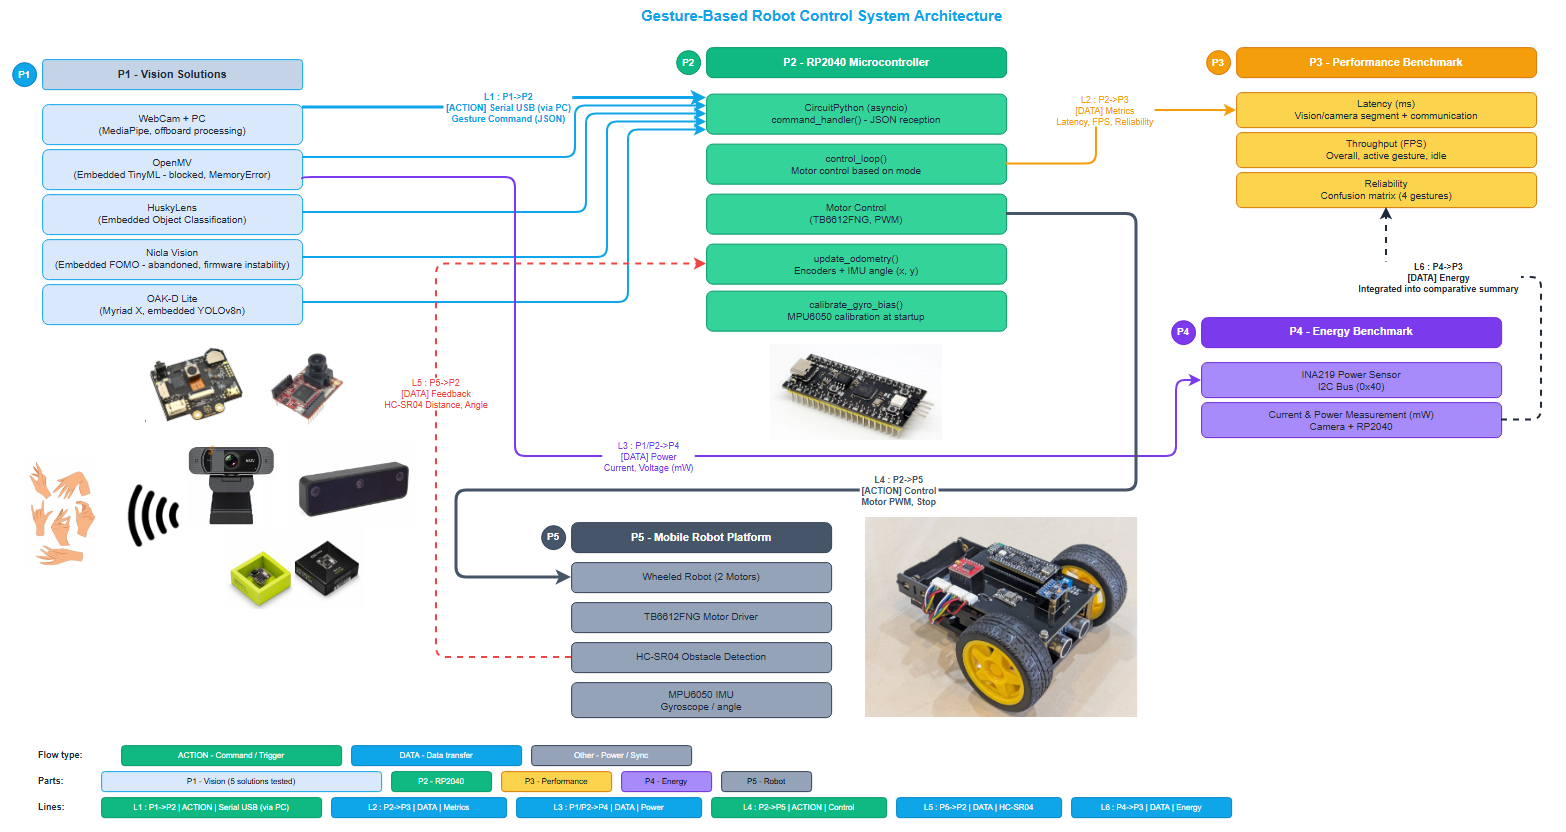
\includegraphics[width=\textheight]{Architecture_Systeme_Benchmark.png}
		\caption{Architecture of the robot gesture-control system (5 vision solutions compared)}
		\label{fig:architecture-benchmark}
	\end{sidewaysfigure}
	
	\subsection*{Required components and software}
	
	\begin{table}[H]
		\centering
		\renewcommand{\arraystretch}{1.5}
		\begin{tabularx}{\textwidth}{|l|X|}
			\hline
			\textbf{Component} & \textbf{Purpose} \\
			\hline
			RP2040 (robot) & Main board of the mobile robot; runs the motor control and receives the gesture commands. \\
			\hline
			Robot chassis + motors (x2) & Mobile platform provided by the laboratory; DC motors controlled by PWM via TB6612FNG. \\
			\hline
			HC-SR04 ultrasonic sensor & Distance/obstacle detection, integrated into the robot's control loop. \\
			\hline
			MPU6050 inertial measurement unit & Measures the robot's angle (gyroscope), used for odometry. \\
			\hline
			Webcam (PC) & Video capture for the WebCam solution; processing offloaded to the PC (MediaPipe). \\
			\hline
			OpenMV Cam M7 (OV7725) & Smart camera: custom TinyML model (Edge Impulse) for gesture recognition. \\
			\hline
			HuskyLens & Smart camera: gesture recognition through embedded \textit{Object Classification}. \\
			\hline
			Arduino Nicla Vision & Miniature artificial-intelligence module: gesture recognition through an embedded FOMO model. \\
			\hline
			OAK-D Lite (Luxonis) & Smart stereo camera: gesture detection through a YOLOv8n model embedded on the Myriad~X chip. \\
			\hline
			INA219 module & Current/voltage measurement over I2C, for the power-consumption metric. \\
			\hline
			USB / serial cables & Firmware flashing, serial communication between the PC, the cameras and the robot. \\
			\hline
		\end{tabularx}
		\caption{Hardware components of the project}
	\end{table}
	
	\begin{table}[H]
		\centering
		\renewcommand{\arraystretch}{1.5}
		\begin{tabularx}{\textwidth}{|p{2.8cm}|p{3.2cm}|X|}
			\hline
			\textbf{Software / Tool} & \textbf{Platform} & \textbf{Purpose} \\
			\hline
			CircuitPython & RP2040 (robot) & Embedded firmware of the robot: reception of JSON commands, motor control, odometry. \\
			\hline
			Thonny & PC $\rightarrow$ RP2040 & Editing and transferring the CircuitPython files onto the robot. \\
			\hline
			OpenCV + MediaPipe & PC & Webcam capture and hand detection (WebCam solution). \\
			\hline
			Edge Impulse & PC $\rightarrow$ OpenMV / Nicla Vision & Training and deployment of the TinyML gesture-recognition models. \\
			\hline
			OpenMV IDE & PC $\rightarrow$ OpenMV / Nicla Vision & MicroPython programming of the cameras based on the OpenMV firmware. \\
			\hline
			HUSKYLENS Python (huskylib) & PC $\rightarrow$ HuskyLens & Official serial-communication library for the HuskyLens. \\
			\hline
			DepthAI (SDK) + Ultralytics YOLO & PC $\rightarrow$ OAK-D Lite & YOLOv8n training, conversion and deployment of the model on the OAK-D Lite camera. \\
			\hline
			pySerial & PC & Serial communication with the robot (JSON command protocol). \\
			\hline
			Python 3 & PC & Benchmark scripts (latency, FPS, reliability, consumption) and export of the results. \\
			\hline
			Git + GitHub & PC & Code versioning and change tracking. \\
			\hline
		\end{tabularx}
		\caption{Software and tools of the project}
	\end{table}
	
	\newpage
	
	%----------------------------------------------------------------------
	%	3.3 Problem statement adopted
	%----------------------------------------------------------------------
	
	\section{Problem statement adopted}
	
	The problem statement adopted for this internship, formalised at the end of this reorientation, is expressed as follows:
	
	\begin{quote}
		\itshape Where should the processing intelligence be placed in a gesture-control chain embedded on an RP2040, and what are the measurable trade-offs between offloaded PC processing, a custom TinyML model and an autonomous smart camera, in terms of latency, throughput, reliability and power consumption?
	\end{quote}
	
	Existing work on the benchmarking of embedded vision each focuses on a single hardware platform and a single processing point, always embedded on the microcontroller, without ever comparing the different possible distributions of processing intelligence. To our knowledge, no study evaluates, for the same mobile-robot gesture-control task, the trade-offs between PC-offloaded processing, a custom embedded TinyML model and a ready-to-use smart camera, by measuring their latency, throughput, recognition reliability and power consumption in a homogeneous way. It is this problem that this internship sought to address, progressively broadening it to five distinct vision architectures.
	
	%----------------------------------------------------------------------
	%	4 STATE OF THE ART / TECHNICAL BACKGROUND
	%----------------------------------------------------------------------
	
\chapter{The five candidate solutions}
	\section{The RP2040 microcontroller}
	
	The RP2040 is a microcontroller designed by the Raspberry Pi Foundation, used as the main board of the IOT Car robot in this project. Its main technical characteristics, summarised in Table~\ref{tab:rp2040-specs}, are taken from its official documentation~\cite{rp2040_datasheet}.
	
	\begin{table}[H]
		\centering
		\small
		\renewcommand{\arraystretch}{1.15}
		\begin{tabularx}{\textwidth}{|l|X|}
			\hline
			\textbf{Characteristic} & \textbf{Value} \\
			\hline
			Processor & Dual-core Arm Cortex-M0+, clocked up to 133~MHz \\
			\hline
			RAM (SRAM) & 264~KB on-chip, split into 6 independent banks for simultaneous access by several masters \\
			\hline
			Program memory (Flash) & No internal flash memory; direct execution from external QSPI flash, up to 16~MB \\
			\hline
			Inputs/outputs (GPIO) & 30 multifunction GPIO pins on the chip \\
			\hline
			Communication interfaces & 2$\times$UART, 2$\times$SPI, 2$\times$I2C \\
			\hline
			PWM & 16 channels (8 slices $\times$ 2 channels) \\
			\hline
			Analogue-to-digital converter (ADC) & 4 channels, 12-bit resolution, up to 500~ksamples/s, with internal temperature sensor \\
			\hline
			PIO (Programmable I/O) & 8 state machines spread across 2 PIO blocks, allowing custom hardware peripherals to be implemented in software \\
			\hline
			USB & Integrated USB 1.1 controller (on-chip PHY), host and device support \\
			\hline
			Power and consumption & Low-power sleep and dormant modes; operating temperature range from $-40$ to $+85\,^{\circ}$C \\
			\hline
		\end{tabularx}
		\caption{Technical characteristics of the RP2040 microcontroller}
		\label{tab:rp2040-specs}
	\end{table}
	
	Two characteristics of this microcontroller directly motivated its use in this project: its dual-core architecture, which makes it possible to distribute the real-time tasks (FreeRTOS) across the two available cores, and its PIO state machines, which offer great flexibility for handling precise protocols or timing signals (for example the distance measurement by the HC-SR04 sensor) without loading the main processor core. In return, the RP2040 has no integrated wireless connectivity (Wi-Fi or Bluetooth), a constraint that rules out a wireless link to the robot.
	
	%----------------------------------------------------------------------
	%	4.2 Study of the camera solutions
	%----------------------------------------------------------------------
	
	\section{Study of the camera solutions (datasheet, architecture, operation)}
	
	This section presents, for each of the five vision solutions compared, a general technical overview (architecture, operating principle) independent of the implementation choices specific to this project, which will be detailed in Chapter~4.
	
	%----------------------------------------------------------------------
	%	4.2.1 Generic WebCam
	%----------------------------------------------------------------------
	
	\subsection{Generic WebCam}
	
	The first solution studied relies on the simplest principle: a standard webcam, with no on-board intelligence, which captures a raw video stream and transmits it entirely to a PC. All of the processing, hand detection, extraction of the characteristic points, gesture classification, is then carried out on the PC side, by the MediaPipe library (whose detailed operation is presented in the following section).
	
	For this project, the webcam used is the one integrated into the laptop used for development, an \textbf{MSI Thin A15 B7VF}~\cite{msi_thina15}.
	
	\begin{figure}[H]
		\centering
		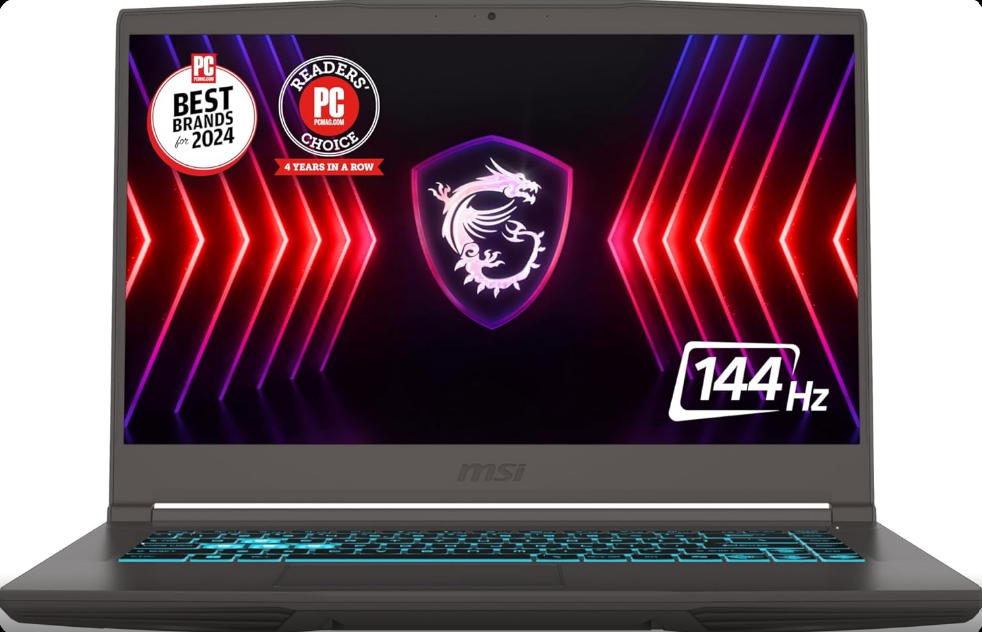
\includegraphics[width=0.6\textwidth]{MSI_ThinA15_Webcam.png}
		\caption{Integrated webcam of the MSI Thin A15 B7VF laptop used for the WebCam solution}
		\label{fig:webcam-msi}
	\end{figure}
	
	\begin{table}[H]
		\centering
		\small
		\renewcommand{\arraystretch}{1.15}
		\begin{tabularx}{\textwidth}{|l|X|}
			\hline
			\textbf{Characteristic} & \textbf{Value} \\
			\hline
			Type & Integrated webcam (laptop) \\
			\hline
			Resolution & HD 720p (1280 $\times$ 720) \\
			\hline
			Connection & Internal (USB bus integrated into the motherboard) \\
			\hline
			Sensor & CMOS, standard laptop webcam type \\
			\hline
			On-board processing & None - raw video capture only \\
			\hline
			Cost & No additional cost (integrated webcam); for comparison, an equivalent generic USB webcam (720p/1080p) costs between €20 and €50 on the market \\
			\hline
		\end{tabularx}
		\caption{Characteristics of the webcam used}
		\label{tab:webcam-specs}
	\end{table}
	
	This complete absence of on-board processing is the defining characteristic of this solution: it represents the simplest and least expensive reference point of the benchmark, but shifts the entire computational load, and therefore the dependence on a PC, onto the processing stage, unlike the smart cameras studied in the following sections.
	
	Since the webcam itself performs no processing, its role in the project is limited to capturing the raw video stream, at a resolution of 1280$\times$720 pixels, transmitted continuously to the PC via the laptop's internal USB bus. This is a deliberately simple choice: this solution requires no additional hardware, no firmware to flash and no model-training phase; only a software library (MediaPipe) is needed on the PC side to extract the useful information from the video stream. It is thus the most accessible reference point of the benchmark, the one that a large number of users could reproduce without any hardware investment, but whose entire processing load, and therefore its dependence on computing power and on the presence of a PC, remains its main drawback compared with the smart cameras studied later.
	
	\newpage
	
	%----------------------------------------------------------------------
	%	4.2.2 OpenMV Cam M7 (OV7725)
	%----------------------------------------------------------------------
	
	\subsection{OpenMV Cam M7 (OV7725)}
	
	The OpenMV Cam M7~\cite{openmv_camm7} is an open-source smart camera, designed to run computer-vision algorithms directly on the board, without requiring a PC for processing. Unlike the webcam studied previously, it embeds its own microcontroller and comes with a dedicated development environment (OpenMV IDE), allowing the board to be programmed in MicroPython.
	
	\begin{figure}[H]
		\centering
		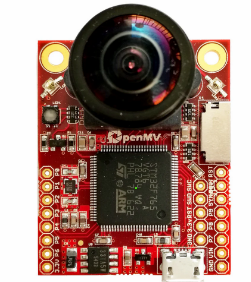
\includegraphics[width=0.5\textwidth]{OpenMV_CamM7.png}
		\caption{OpenMV Cam M7 camera (OV7725 sensor) used for the project}
		\label{fig:openmv-m7}
	\end{figure}
	
	\begin{table}[H]
		\centering
		\small
		\renewcommand{\arraystretch}{1.15}
		\begin{tabularx}{\textwidth}{|l|X|}
			\hline
			\textbf{Characteristic} & \textbf{Value} \\
			\hline
			Microcontroller & STM32F765VI, ARM Cortex-M7 clocked up to 216~MHz \\
			\hline
			RAM & 512~KB \\
			\hline
			Flash memory & 2~MB (internal); optional microSD card for additional storage \\
			\hline
			Image sensor & OmniVision OV7725: 640$\times$480 in 8-bit greyscale, or 320$\times$240 in RGB565 colour, up to 30 to 60~fps depending on the resolution \\
			\hline
			Interfaces & USB (virtual serial port), SPI, I2C, UART, CAN, 12-bit ADC/DAC, servo outputs \\
			\hline
			Consumption (@3.3~V) & About 110~mA at rest, 190 to 200~mA in active operation \\
			\hline
			Programming environment & MicroPython, via the dedicated OpenMV IDE \\
			\hline
			Price & Around US\$55 at launch (model now replaced by the OpenMV Cam H7 range, which is newer and more powerful) \\
			\hline
		\end{tabularx}
		\caption{Characteristics of the OpenMV Cam M7}
		\label{tab:openmv-specs}
	\end{table}
	
	The main appeal of this solution lies in its ability to run an artificial-intelligence model directly on-board the camera, allowing in theory a fully autonomous gesture recognition, with no dependence on a PC while operating, unlike the WebCam solution. This characteristic comes, however, with a strong constraint: the amount of RAM available to run a machine-learning model is much more limited than on a PC, which, as detailed in Chapter~4, proved to be a decisive factor for this solution.
	
	%----------------------------------------------------------------------
	%	4.2.3 Nicla Vision
	%----------------------------------------------------------------------
	
	\subsection{Arduino Nicla Vision}
	
	The Arduino Nicla Vision~\cite{arduino_niclavision} is a very small embedded artificial-intelligence module, designed for computer vision and machine learning at the network edge. Although produced by Arduino, it shares the same programming environment as the OpenMV Cam studied previously, since it can be programmed with the OpenMV firmware in MicroPython.
	
	\begin{figure}[H]
		\centering
		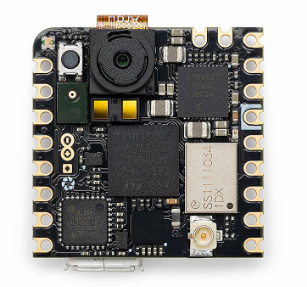
\includegraphics[width=0.4\textwidth]{Nicla_Vision.png}
		\caption{Arduino Nicla Vision module used for the project}
		\label{fig:nicla-vision}
	\end{figure}
	
	\begin{table}[H]
		\centering
		\small
		\renewcommand{\arraystretch}{1.15}
		\begin{tabularx}{\textwidth}{|l|X|}
			\hline
			\textbf{Characteristic} & \textbf{Value} \\
			\hline
			Microcontroller & STM32H747AII6, dual-core Arm Cortex-M7 up to 480~MHz and Cortex-M4 up to 240~MHz \\
			\hline
			RAM & 1~MB \\
			\hline
			Flash memory & 2~MB \\
			\hline
			Image sensor & GC2145, 2~megapixel colour sensor \\
			\hline
			Additional sensors & 6-axis inertial measurement unit, integrated MEMS microphone, time-of-flight distance sensor \\
			\hline
			Connectivity & Integrated Wi-Fi 802.11 b/g/n and Bluetooth \\
			\hline
			Dimensions & 22.86~$\times$~22.86~mm \\
			\hline
			Power supply & USB or battery, suited to autonomous use \\
			\hline
			Programming environment & MicroPython (OpenMV firmware) or Arduino IDE (C/C++), compatible with Edge Impulse \\
			\hline
			Price & Around €95 to €115 depending on the reseller \\
			\hline
		\end{tabularx}
		\caption{Characteristics of the Arduino Nicla Vision}
		\label{tab:nicla-specs}
	\end{table}
	
	Its extremely small size and its integrated wireless connectivity make it a solution particularly well suited to autonomous embedded applications. Its processor, much more powerful than that of the OpenMV Cam M7, suggested a better margin for running a gesture-recognition model. This solution nevertheless shares the same OpenMV firmware as the camera studied previously, which potentially exposes it to the same software limitations, as will be analysed in Chapter~4.
	
	%----------------------------------------------------------------------
	%	4.2.4 HuskyLens
	%----------------------------------------------------------------------
	
	\subsection{HuskyLens}
	
	The HuskyLens, developed by DFRobot~\cite{dfrobot_huskylens}, is a smart camera designed to make artificial intelligence accessible without complex programming. It includes a screen and physical buttons allowing the embedded algorithms to be trained and configured directly, without requiring a PC for the usage phase.
	
	\begin{figure}[H]
		\centering
		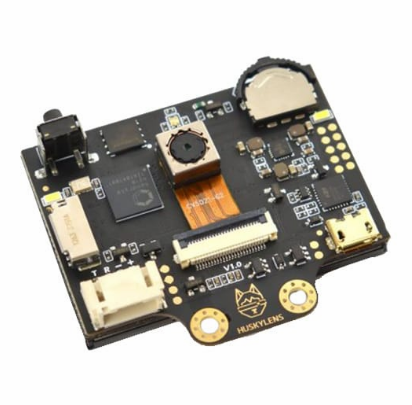
\includegraphics[width=0.4\textwidth]{HuskyLens.png}
		\caption{HuskyLens camera used for the project}
		\label{fig:huskylens}
	\end{figure}		
	
	\begin{table}[H]
		\centering
		\small
		\renewcommand{\arraystretch}{1.15}
		\begin{tabularx}{\textwidth}{|l|X|}
			\hline
			\textbf{Characteristic} & \textbf{Value} \\
			\hline
			Processor & Kendryte K210, dual-core 64-bit RISC-V up to 400~MHz, with dedicated neural processing unit (about 1~TOPS) \\
			\hline
			Image sensor & OV2640, 2~megapixels \\
			\hline
			Screen & Integrated 2-inch IPS panel, 320$\times$240 resolution \\
			\hline
			Interfaces & UART (9600 to 115200~bps), I2C (100 to 400~kHz) \\
			\hline
			Power supply & 3.3 to 5.0~V, consumption of about 230 to 320~mA depending on the mode used \\
			\hline
			Dimensions & 52~$\times$~44.5~mm \\
			\hline
			Embedded algorithms & Face recognition, object tracking, object recognition, line tracking, colour recognition, tag recognition, object classification \\
			\hline
			Price & US\$34.90 (official DFRobot store) \\
			\hline
		\end{tabularx}
		\caption{Characteristics of the HuskyLens}
		\label{tab:huskylens-specs}
	\end{table}
	
	Unlike the OpenMV Cam and the Nicla Vision, the HuskyLens is not used by writing inference code. Training is done directly on the device, through incremental learning using the dedicated button, the chosen algorithm (object classification in this project) then being run continuously on the board. Once trained, it transmits only the recognition result (the identifier of the detected class) over its serial port, which considerably simplifies its integration with an external microcontroller, as detailed in Chapter~4.
	
	\newpage
	
	%----------------------------------------------------------------------
	%	4.2.5 OAK-D Lite (Luxonis)
	%----------------------------------------------------------------------
	
	\subsection{OAK-D Lite (Luxonis)}
	
	The OAK-D Lite, developed by Luxonis~\cite{luxonis_oakdlite}, is a smart stereo camera intended for advanced computer-vision applications, combining depth perception and the execution of neural networks directly on the camera. It is the most advanced solution of the benchmark in terms of on-board computing power.
	
	\begin{figure}[H]
		\centering
		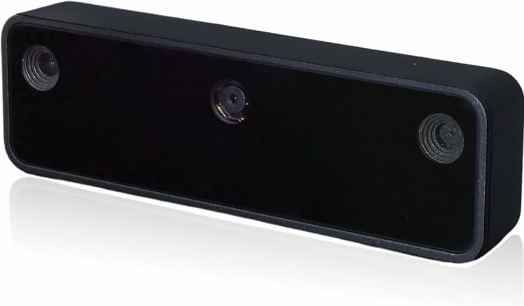
\includegraphics[width=0.5\textwidth]{OAKD_Lite.png}
		\caption{OAK-D Lite camera used for the project}
		\label{fig:oakd-lite}
	\end{figure}
	
	\begin{table}[H]
		\centering
		\small
		\renewcommand{\arraystretch}{1.15}
		\begin{tabularx}{\textwidth}{|l|X|}
			\hline
			\textbf{Characteristic} & \textbf{Value} \\
			\hline
			Vision processor & Intel Movidius Myriad X VPU, up to 4~TOPS, of which 1.4~TOPS dedicated to neural-network inference \\
			\hline
			On-board cameras & Two OV7251 monochrome cameras (640$\times$480, global shutter) for stereo vision, combined with a central IMX214 colour camera (13~megapixels) \\
			\hline
			Depth perception & Stereo depth map, up to 300,000 points \\
			\hline
			Video encoding & H.264, H.265, MJPEG, up to 4K/30~fps or 1080p/60~fps \\
			\hline
			Connection & USB-C (USB 3.1 Gen1) \\
			\hline
			Dimensions & 91~$\times$~28~$\times$~17.5~mm \\
			\hline
			Development environment & DepthAI framework (open source), model conversion via OpenVINO \\
			\hline
			Power supply & No external power; powered solely through the USB-C port \\
			\hline
			Price & Around US\$99 \\
			\hline
		\end{tabularx}
		\caption{Characteristics of the OAK-D Lite}
		\label{tab:oakd-specs}
	\end{table}
	
	\newpage
	
	Unlike the three other smart cameras studied, the OAK-D Lite is not limited to running a pre-trained model or one trained by incremental learning. It is designed to run more complex deep neural-network architectures, converted specifically for its Myriad X processor, opening the way to modern object-detection models such as YOLO. This higher computing power comes, however, with a markedly more complex training and deployment chain, as detailed in Chapter~4.
	
	%----------------------------------------------------------------------
	%	4.3 Preliminary comparative synthesis
	%----------------------------------------------------------------------
	
	\section{Preliminary comparative synthesis}
	
	A summary table makes it possible to visualise at a glance the differences between the five solutions, and the text that follows allows hypotheses to be formulated even before any measurement results are available, which will give more meaning to Chapter~5 once these hypotheses are confronted with the actual results.
	
	\begin{table}[H]
		\centering
		\footnotesize
		\renewcommand{\arraystretch}{1.05}
		\begin{tabularx}{\textwidth}{|l|X|X|X|l|}
			\hline
			\textbf{Solution} & \textbf{Processing / computing power} & \textbf{Available memory} & \textbf{Typical consumption} & \textbf{Price} \\
			\hline
			WebCam + MediaPipe & Offloaded to the PC, power depending on the computer used & Depends on the PC & Not measurable on the camera itself & €0 (integrated) \\
			\hline
			OpenMV Cam M7 & Embedded, Cortex-M7 216~MHz, no dedicated AI accelerator & 512~KB RAM & 110 to 200~mA & Around US\$55 \\
			\hline
			Nicla Vision & Embedded, Cortex-M7 480~MHz + Cortex-M4 240~MHz, no dedicated AI accelerator & 1~MB RAM & Not documented by the manufacturer & Around €95 to €115 \\
			\hline
			HuskyLens & Embedded, K210 400~MHz, with dedicated NPU (about 1~TOPS) & 8~MB SRAM (of which 2~MB dedicated to the NPU) & 230 to 320~mA & Around US\$35 \\
			\hline
			OAK-D Lite & Embedded, Myriad~X VPU, 4~TOPS (of which 1.4~TOPS dedicated to AI) & 512~MB DRAM + 2.5~MB dedicated internal memory & Not documented by the manufacturer & Around US\$99 \\
			\hline
		\end{tabularx}
		\caption{Comparative synthesis of the technical characteristics of the five solutions}
		\label{tab:synthese-preliminaire}
	\end{table}
	
	\newpage
	
	On the basis of these characteristics alone, several predictions can be made.\\
	
	Regarding latency and throughput, the WebCam solution benefits from the computing power of a PC, far greater than that of any smart camera, but this advantage could be partly offset by going through a USB link and by a heavier software library (MediaPipe).\newline
	The OAK-D Lite has the largest gap in raw computing power (4~TOPS) and a memory reserve far greater than that of the other embedded solutions, which suggests that it could offer good performance once the model is optimised, despite a more complex processing chain.\newline 
	The HuskyLens, with a modest but dedicated NPU and a deliberately simple classification algorithm, could prove particularly fast despite its low raw computing power.\newline
	The OpenMV Cam M7 and the Nicla Vision, lacking a dedicated hardware AI accelerator, seem less well positioned on this point, the former being furthermore strongly constrained by its small amount of RAM.\\
	
	Regarding recognition reliability, it is harder to make a prediction from the datasheets alone, since recognition quality depends more on the training of the model than on the raw power of the hardware. It can nevertheless be assumed that a larger memory margin (Nicla Vision, OAK-D Lite) would allow the use of more complex, and potentially more accurate, models than those constrained by the 512~KB of the OpenMV Cam M7.\\
	
	Regarding power consumption, the OAK-D Lite, which embeds three image sensors and external DRAM, is probably the most power-hungry solution of the benchmark, although the manufacturer does not provide a precise figure. The OpenMV Cam M7 seems, a priori, the most frugal among the smart cameras, with a measured consumption of between 110 and 200~mA.\\
	
	These predictions remain working hypotheses, to be confronted with the results measured in the benchmark protocol detailed in Chapter~4.
	
	\newpage
	
	%----------------------------------------------------------------------
	%	5 APPROACH AND WORK CARRIED OUT ON THE RESEARCH TOPIC
	%----------------------------------------------------------------------
	
\chapter{Test bench: robot and communication protocol}
	\section{Hardware architecture of the robot (IOT Car)}
	
	The robot used for the entire benchmark is the IOT Car robot, a two-wheel-drive platform provided by the laboratory and first used during an introductory workshop. Its control board is an RP2040, programmed in CircuitPython following an asynchronous architecture (\texttt{asyncio}). This section explains the role and operation of the three code files provided with the platform (\texttt{robot.py}, \texttt{pio\_encoder.py}, \texttt{pid\_controller.py}), whose full code is available in the Code Appendix.
	
	\begin{figure}[H]
		\centering
		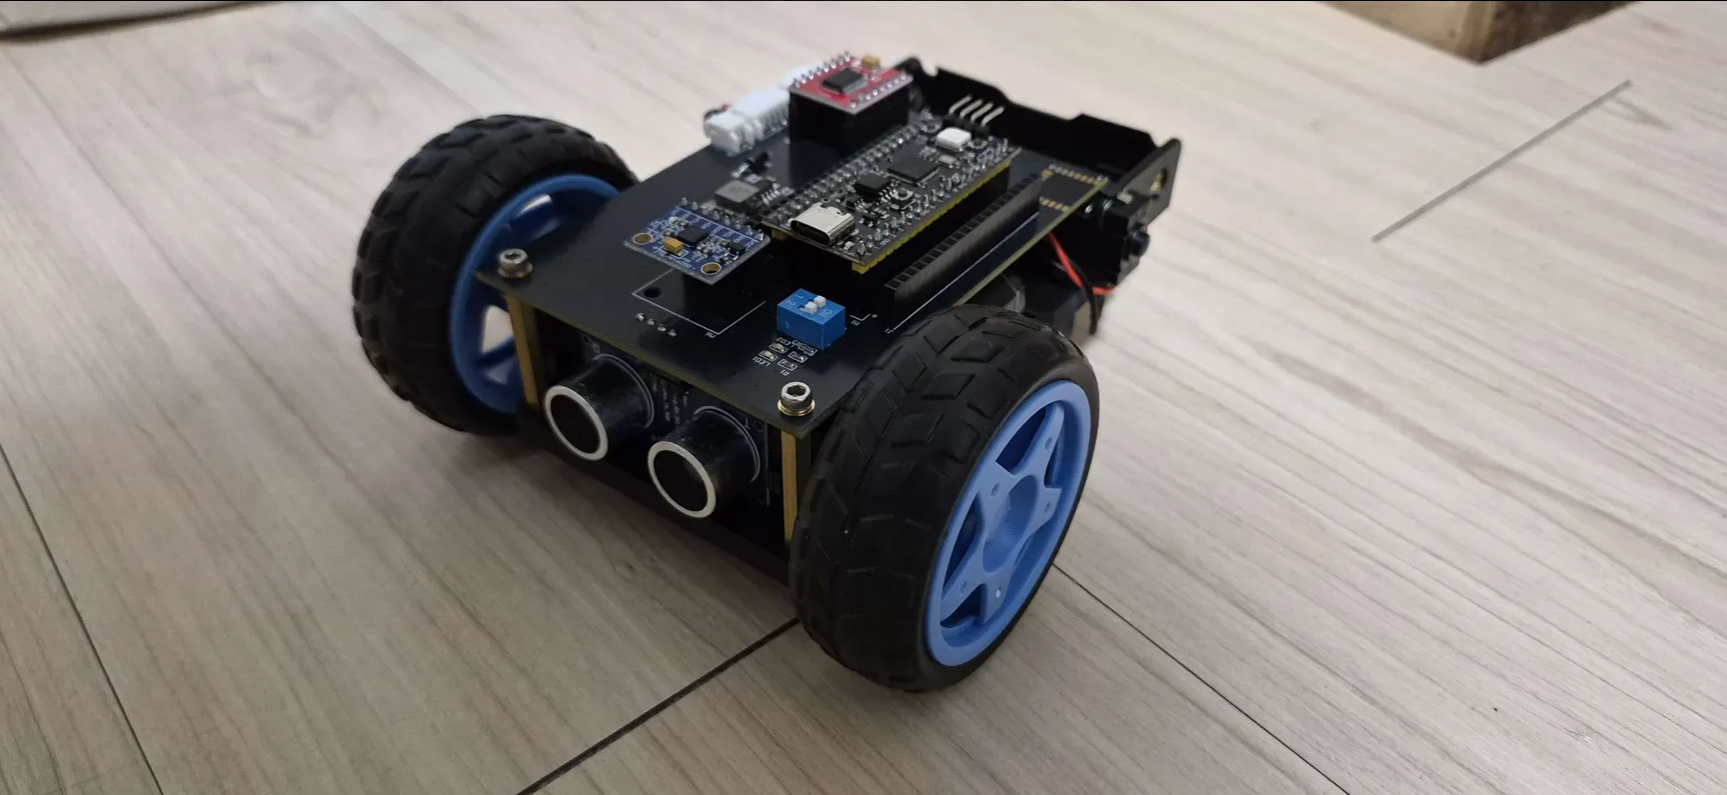
\includegraphics[width=0.7\textwidth]{IOT_Car_Robot.png}
		\caption{IOT Car robot, identical to the one used in the workshop}
		\label{fig:iotcar-robot-bench}
	\end{figure}
	
	\newpage
	
	\subsection*{Motor control (\texttt{robot.py})}
	
	The role of this file is to drive the robot's two DC motors, each controlled by a dual H-bridge driver of the TB6612FNG type, according to the mapping shown in Table~\ref{tab:pinout-robot}.
	
	\begin{table}[H]
		\centering
		\small
		\renewcommand{\arraystretch}{1.15}
		\begin{tabularx}{\textwidth}{|l|l|X|}
			\hline
			\textbf{RP2040 pin} & \textbf{Function} & \textbf{Role} \\
			\hline
			GP16 & Left motor PWM & Left motor speed \\
			\hline
			GP17, GP18 & Left motor direction & Rotation direction of the left motor \\
			\hline
			GP19 & Standby (STBY) & Global enable of the TB6612FNG driver \\
			\hline
			GP20, GP21 & Right motor direction & Rotation direction of the right motor \\
			\hline
			GP22 & Right motor PWM & Right motor speed \\
			\hline
			GP26, GP27 & Left encoder & Reading of the left wheel rotation (PIO) \\
			\hline
			GP28, GP29 & Right encoder & Reading of the right wheel rotation (PIO) \\
			\hline
			GP4, GP5 & HC-SR04 (trigger, echo) & Distance measurement at the front of the robot \\
			\hline
			GP6, GP7 & I2C0 (SDA, SCL) & Communication with the MPU6050 inertial measurement unit \\
			\hline
		\end{tabularx}
		\caption{Mapping of the RP2040 pins on the IOT Car robot}
		\label{tab:pinout-robot}
	\end{table}
	
	The \texttt{set\_speed()} function receives a target speed between $-1$ and $1$. Its sign sets the state of the two direction pins (forward rotation, backward, or stop if zero), while its absolute value is converted into a 16-bit PWM duty cycle according to the formula
	
	\begin{equation}
		\text{duty\_cycle} = \left\lfloor \left(2^{16}-1\right) \times \min\left(|v|,\,1\right) \right\rceil
		\label{eq:pwm}
	\end{equation}
	
	where $v$ is the target speed. The \texttt{set\_left()}, \texttt{set\_right()} and \texttt{set\_all()} functions make it possible to drive a single motor or both simultaneously, while \texttt{stop()} cuts all outputs.
	
	\subsection*{Odometry using encoders and PIO (\texttt{pio\_encoder.py})}
	
	Each wheel is fitted with a quadrature encoder, made up of two channels (A and B) delivering square signals phase-shifted relative to one another. Reliably reading this type of sensor normally requires very frequent monitoring of both pins, so as not to miss any transition, which would represent a significant load on the processor if it were done in pure software. The \texttt{pio\_encoder.py} file works around this constraint by exploiting the PIO state machines of the RP2040, presented in the technical overview in Section~2.1.
	
	The PIO assembly program runs completely independently of the processor core: at each cycle, it reads the current state of the two encoder pins and compares it to the previously read state. When a transition is detected, the program observes the state of the second channel at the precise moment of this transition to determine whether the wheel is turning forwards or backwards, then increments or decrements an internal counter accordingly, which is transmitted at regular intervals to a hardware queue (FIFO) accessible from CircuitPython. On the software side, the \texttt{QuadratureEncoder} class runs an asynchronous task that regularly empties this queue to keep the counter value up to date, accessible via the \texttt{read()} method. A \texttt{reversed} parameter makes it possible to invert the counting direction of an encoder, which is necessary for the right encoder since the two wheels are mounted as mirror images of one another.\\
	
	This raw count is then converted into a distance travelled from the mechanical characteristics of the robot. With a wheel diameter $D_w = 65$~mm, the wheel circumference is:
	
	\begin{equation}
		C_w = \pi \times D_w \approx 204.20\ \text{mm}
		\label{eq:circumference}
	\end{equation}
	
	The motor drives the wheel through a reduction gear with ratio $N_{\text{red}} = 90$, and the encoder generates $P_{\text{enc}} = 52$ pulses per motor revolution. The number of pulses corresponding to one full wheel revolution is therefore:
	
	\begin{equation}
		T_{\text{rev}} = P_{\text{enc}} \times N_{\text{red}} = 52 \times 90 = 4680\ \text{pulses/revolution}
		\label{eq:ticks-per-rev}
	\end{equation}
	
	hence a distance travelled per pulse of
	
	\begin{equation}
		d_{\text{tick}} = \frac{C_w}{T_{\text{rev}}} \approx \frac{204.20}{4680} \approx 0.04364\ \text{mm/pulse} \approx 4.364 \times 10^{-5}\ \text{m/pulse}
		\label{eq:tick-distance}
	\end{equation}
	
	The total distance travelled by a wheel after $n$ counted pulses is then simply $d = n \times d_{\text{tick}}$.
	
	\subsection*{On-board sensors}
	
	The robot has two additional sensors. An HC-SR04 ultrasonic distance sensor, mounted at the front of the robot, allows obstacle detection. An MPU6050 inertial measurement unit, connected over I2C, provides the robot's angle by integrating the gyroscope data.
	
	\subsection*{PID control (\texttt{pid\_controller.py})}
	
	This file provides a generic implementation of a PID controller (proportional, integral, derivative), intended to control the speed or trajectory of the robot from the odometry feedback presented above. The classic continuous form of a PID controller is written
	
	\begin{equation}
		u(t) = K_p\,e(t) + K_i \int_0^{t} e(\tau)\,d\tau + K_d \,\frac{de(t)}{dt}
		\label{eq:pid-continu}
	\end{equation}
	
	where $e(t)$ is the error between the setpoint and the measurement, and $K_p$, $K_i$, $K_d$ the proportional, integral and derivative gains. Since the controller is run at discrete intervals $\Delta t$ (\texttt{calculate(error, dt)} method), the integral term is approximated using the rectangle method
	
	\begin{equation}
		I_n = I_{n-1} + e_n \, \Delta t
		\label{eq:pid-integral}
	\end{equation}
	
	this value then being bounded within the interval $[I_{\min}, I_{\max}]$ (\texttt{imin}, \texttt{imax} parameters). This saturation prevents the \textit{windup} phenomenon: without it, a large error maintained over a long period (for example a robot stuck against an obstacle) would make the integral term diverge well beyond what is physically useful, causing a large overshoot of the setpoint once the obstacle is removed.
	
	For the derivative term, the code does not directly apply the raw difference of the error between two instants, which would strongly amplify measurement noise. A filtered version of the error is maintained by a first-order low-pass filter (exponential moving average)
	
	\begin{equation}
		\bar{e}_n = \bar{e}_{n-1} + \alpha \left(e_n - \bar{e}_{n-1}\right), \qquad \alpha = \texttt{d\_filter\_gain} \in [0,1]
		\label{eq:pid-filter}
	\end{equation}
	
	and the derivative term is computed from the increment of this filtered error
	
	\begin{equation}
		D_n = \frac{\bar{e}_n - \bar{e}_{n-1}}{\Delta t} = \frac{\alpha \left(e_n - \bar{e}_{n-1}\right)}{\Delta t}
		\label{eq:pid-derivative}
	\end{equation}
	
	The controller output, returned by \texttt{calculate()}, is finally
	
	\begin{equation}
		u_n = K_p\,e_n + K_i\,I_n + K_d\,D_n
		\label{eq:pid-sortie}
	\end{equation}
	
	The full code of the three files presented in this section is available in the Code Appendix.
	
	\newpage
	
	%----------------------------------------------------------------------
	%	5.2 Communication protocol (UART/JSON)
	%----------------------------------------------------------------------
	
	\section{Communication protocol (UART/JSON)}
	
	Since the wireless link was ruled out back in Section~2.1 (no Wi-Fi chip on the RP2040), communication between the control station (PC or smart camera depending on the solution) and the robot relies on a wired serial link. The RP2040 board natively exposes, through CircuitPython, a USB serial port (\texttt{usb\_cdc}) on the same physical connection as the one used for programming, which avoids any additional wiring.
	
	\subsection*{Message format}
	
	The commands are transmitted as JSON messages, one message per line, sent over the serial port and read on the robot side via \texttt{sys.stdin.readline()}, in a \texttt{command\_handler()} function of the main file \texttt{code.py}, which then relies on the functions of \texttt{robot.py} presented in Section~3.1 (\texttt{set\_left()}, \texttt{set\_right()}, \texttt{set\_all()}, \texttt{stop()}). Four commands were defined, summarised in Table~\ref{tab:protocole-json}.
	
	\begin{table}[H]
		\centering
		\small
		\renewcommand{\arraystretch}{1.2}
		\begin{tabular}{ll}
			\toprule
			\textbf{JSON message} & \textbf{Effect on the robot} \\
			\midrule
			\texttt{\{"cmd": "forward"\}} & Moves forward continuously \\
			\texttt{\{"cmd": "stop"\}} & Immediate stop \\
			\texttt{\{"cmd": "turn\_left"\}} & Gradual left turn \\
			\texttt{\{"cmd": "turn\_right"\}} & Gradual right turn \\
			\bottomrule
		\end{tabular}
		\caption{JSON command protocol between the control station and the robot}
		\label{tab:protocole-json}
	\end{table}
	
	\subsection*{General orchestration (\texttt{code.py})}
	
	The \texttt{code.py} file is the main program run on the robot; it imports \texttt{robot.py} and \\ \texttt{pid\_controller.py}, and orchestrates all of the asynchronous tasks. At startup, the \texttt{main()} function launches \texttt{control\_loop()}, which itself starts\\ \texttt{command\_handler()} as a concurrent task via \texttt{asyncio.create\_task()}. The two tasks thus run in parallel: \texttt{command\_handler()} continuously monitors the serial port to update the robot's current state (\texttt{state["mode"]}), while \texttt{control\_loop()} actually drives the motors at a regular rate (one iteration every 100~ms).
	
	Before starting the control loop, the robot runs a gyroscope calibration phase: the \texttt{calibrate\_gyro\_bias()} function averages 100 gyroscope measurements taken 5~ms apart, with the robot stationary, in order to estimate its static bias $b$. This bias is then subtracted from each new measurement to limit the drift of the computed angle over time. The robot's angle is then updated at each iteration of the control loop by integrating the angular velocity of the gyroscope, according to
	
	\begin{equation}
		\theta_n = \theta_{n-1} + \left(\omega_n - b\right) \times \frac{180}{\pi} \times \Delta t
		\label{eq:angle-gyro}
	\end{equation}
	
	where $\theta_n$ is the current angle (in degrees), $\omega_n$ the angular velocity measured by the gyroscope (in rad/s) about the vertical axis, $b$ the bias estimated during calibration, and $\Delta t$ the time elapsed since the last iteration.
	
	The robot's position is estimated by odometry, from the encoders presented in Section~3.1 and the angle computed above. At each iteration, the distance travelled by each wheel since the last update is computed from the change in pulse count, converted to metres via $d_{\text{tick}}$ (Equation~\ref{eq:tick-distance}), then the position is updated according to
	
	\begin{equation}
		d_n = \frac{\Delta_{\text{left}} + \Delta_{\text{right}}}{2}, \qquad
		\begin{cases}
			x_n = x_{n-1} + d_n \cos(\theta_n) \\
			y_n = y_{n-1} + d_n \sin(\theta_n)
		\end{cases}
		\label{eq:odometrie}
	\end{equation}
	
	This formulation amounts to treating, at each time step, the robot's displacement as a straight-line segment oriented along the current angle, an approximation that is valid here given the short time interval between two iterations (100~ms).
	
	At each iteration, the control loop also reads the distance measured by the HC-SR04 sensor, handling the case where no echo is received (no obstacle), applies the timeout safety mechanism described below, drives the motors according to the current state (\texttt{state["mode"]}), then sends back a telemetry line over the serial port (position, angle, current mode, measured distance), useful for monitoring and debugging the robot during the tests.
	
	\subsection*{Behaviour adopted}
	
	The chosen behaviour relies on continuous motion rather than on discrete commands. The control station resends the current command at a regular interval, roughly every 150~ms, as long as the corresponding gesture is detected. If no gesture is recognised, or if more than 0.4~seconds elapse without a new command being received by the robot (\texttt{COMMAND\_TIMEOUT} constant), the robot stops automatically. This safety mechanism prevents a robot left to itself from continuing to move forward in the event of a loss of the serial link, of the hand leaving the camera's field of view, or of a freeze on the PC side.
	
	An extension of this protocol, added later for the needs of the latency measurement, also makes it possible to exchange \texttt{\{"ping": n\}} messages to which the robot immediately replies with \texttt{\{"pong": n\}}, directly from \texttt{command\_handler()}, before any processing related to movement. The operation of this extension is detailed in the benchmark protocol presented in the following sections.
	
	\newpage
	
	%----------------------------------------------------------------------
	%	5.3 WebCam + MediaPipe
	%----------------------------------------------------------------------
	
\chapter{Implementation and measurements, solution by solution}
	\section{WebCam + MediaPipe}
	
	\subsection*{Principle and software environment}
	
	This first solution aims to control the IOT Car robot remotely using hand gestures, captured by the laptop webcam presented in Section~2.2.1. The PC analyses the video stream, recognises one gesture out of four, translates it into a movement command, then transmits this command to the robot according to the protocol established in Section~3.2.
	
	Development on the PC side is done in Python 3.11. Three libraries are installed via \texttt{pip}: \texttt{opencv-python} for capturing and displaying the video stream, \texttt{mediapipe} for hand detection and landmark extraction, and \texttt{pyserial} for communication with the robot over the USB serial port.
	
	The development followed a four-step progression, each adding a feature to the previous one: validation of the webcam (\texttt{webcam\_test.py}), hand detection and finger counting (\texttt{gesture\_test.py}), precise classification of the four gestures (\texttt{gesture\_command.py}), then sending the commands to the robot over the serial link \\ (\texttt{gesture\_to\_serial.py}), later enriched with a real-time dashboard in the final version (\texttt{gesture\_to\_serial\_Dashbord\_upg.py}).
	
	\subsection*{Hand detection with MediaPipe}
	
	Hand detection relies on MediaPipe~\cite{mediapipe_hands}, an open-source framework developed by Google, through its \texttt{solutions.hands} module. This module is based on a two-stage pipeline. A first model, the palm detector, analyses the full image and locates the palm as an oriented bounding box, the palm being simpler to detect reliably than the whole hand, whose shape varies greatly depending on whether the fingers are folded or extended. A second model, applied only to the region cropped around the detected palm, then predicts by direct regression the coordinates of 21 characteristic points of the hand (wrist, joints and tips of each finger), in three dimensions.
	
	One practical point is worth noting: recent versions of MediaPipe (0.10.31 and above) present a known regression that makes the \texttt{solutions} module inaccessible \\ (\texttt{AttributeError: module 'mediapipe' has no attribute 'solutions'}), documented in the project's official repository~\cite{mediapipe_issue6200}. Version 0.10.14 was therefore installed specifically for this project.
	
	\subsection*{Gesture classification}
	
	The \texttt{get\_finger\_states()} function determines, for each finger, whether it is raised or folded, from the coordinates of the 21 points provided by MediaPipe. For the four fingers other than the thumb, the state is obtained by comparing the vertical coordinate ($y$) of the fingertip (\textit{tip}) with that of the joint located two levels below; the finger is considered raised if its tip is above this joint in the image. The thumb, whose anatomy does not allow this same vertical comparison, is handled separately by a horizontal comparison ($x$) between its tip and the adjacent joint, the direction of the comparison depending on the detected hand (left or right), provided by MediaPipe.
	
	The \texttt{classify\_gesture()} function then maps the resulting tuple of the five finger states to one of the four defined gestures, summarised in Table~\ref{tab:gestes-webcam}.
	
	\begin{table}[H]
		\centering
		\small
		\begin{tabular}{lll}
			\toprule
			\textbf{Gesture} & \textbf{Raised fingers (T-I-M-R-P)} & \textbf{Command} \\
			\midrule
			Closed fist & 0-0-0-0-0 & Forward \\
			Open hand & 1-1-1-1-1 & Stop \\
			Index + thumb & 1-1-0-0-0 & Turn left \\
			Index + pinky & 0-1-0-0-1 & Turn right \\
			\bottomrule
		\end{tabular}
		\caption{Correspondence between the recognised gestures and the robot commands}
		\label{tab:gestes-webcam}
	\end{table}
	
	\begin{figure}[H]
		\centering
		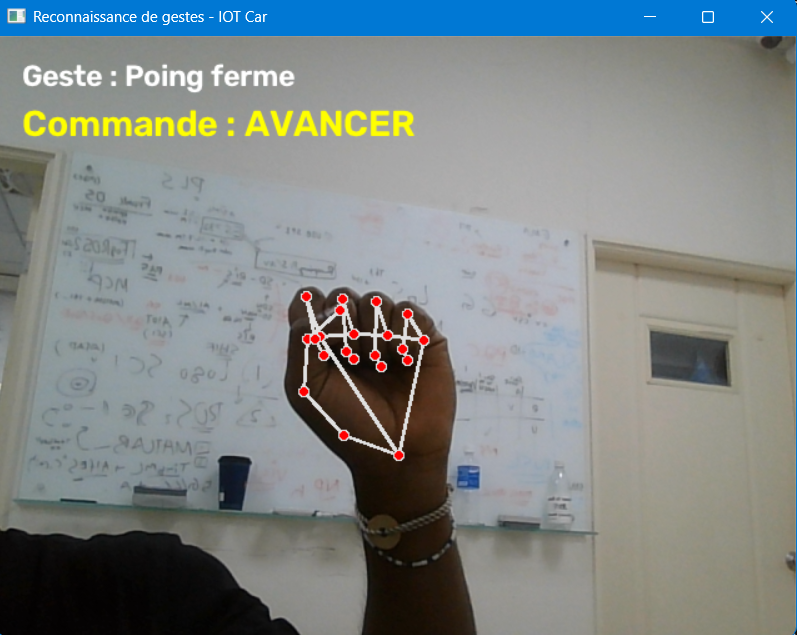
\includegraphics[width=0.45\textwidth]{Webcam/capture_poing_ferme.png}
		\hfill
		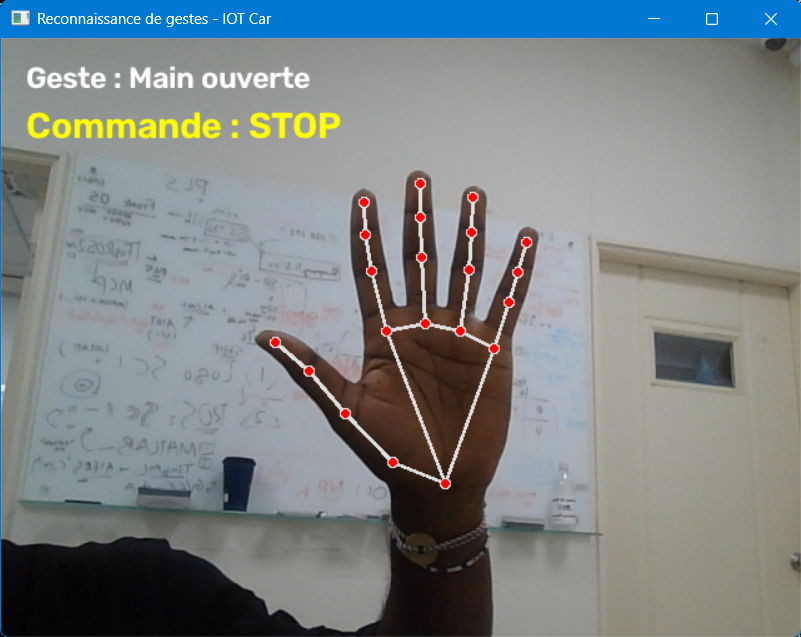
\includegraphics[width=0.45\textwidth]{Webcam/capture_main_ouverte.png}
		\caption{``Closed fist'' (forward) and ``open hand'' (stop) gestures}
		\label{fig:gestes-webcam-1}
	\end{figure}
	
	\begin{figure}[H]
		\centering
		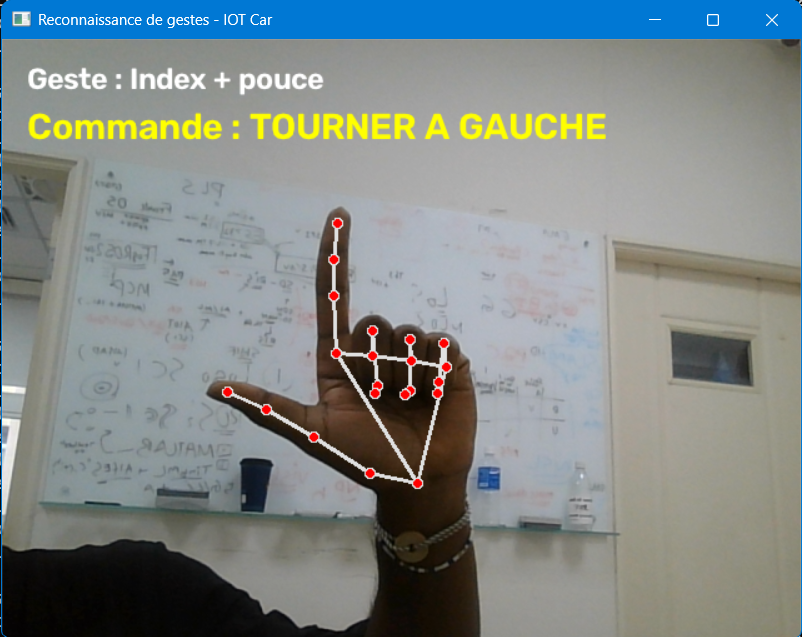
\includegraphics[width=0.45\textwidth]{Webcam/capture_index_pouce.png}
		\hfill
		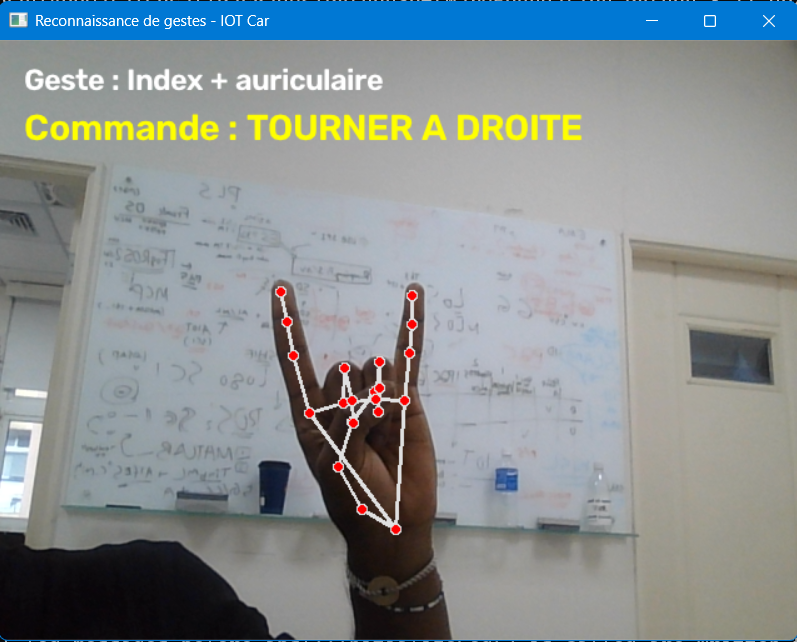
\includegraphics[width=0.45\textwidth]{Webcam/capture_index_auriculaire.png}
		\caption{``Index + thumb'' (left) and ``index + pinky'' (right) gestures}
		\label{fig:gestes-webcam-2}
	\end{figure}
	
	\subsection*{Transmission of the commands to the robot}
	
	Once the gesture is classified, the \texttt{build\_json\_command()} function builds the corresponding JSON message, transmitted to the robot according to the protocol defined in Section~3.2. If no hand is detected in the image, the command sent is \texttt{stop} by default, guaranteeing that the robot stops as soon as the hand leaves the camera's field of view. The current command is resent at a regular interval (\texttt{SEND\_INTERVAL}, 150~ms), and immediately whenever it changes, in order to guarantee both continuous motion and good responsiveness to gesture changes.
	
	At startup of the script, a reset sequence is sent to the robot (interruption of the running code, exit from the \textit{raw REPL} if necessary, then software restart), so as to guarantee that the robot is indeed running \texttt{code.py} before command sending begins. On the reading side, the messages coming from the robot are filtered to ignore the echo of the sent commands, and the display of status messages is limited to twice per second so as not to overload the console.
	
	\subsection*{Difficulties encountered and solutions applied}
	
	This first integration, carried out with the WebCam solution before the other four, made it possible to solve several difficulties common to the whole project, the robot's embedded code then remaining unchanged for the following solutions.
	
	\begin{itemize}
		\item \textbf{Robot stuck in the interactive console.} After an editing session in Thonny, the robot sometimes remained at the interactive prompt instead of running \texttt{code.py}, interpreting the JSON commands as literal Python code. An automatic software restart was added at serial connection.
		\item \textbf{Robot stuck in \textit{raw REPL} mode.} A second freeze appeared after deleting a file via Thonny, which internally uses a serial mode that disables the automatic execution of \texttt{code.py}. An explicit exit from this mode was added before the software restart.
		\item \textbf{\texttt{CIRCUITPY} disk write-protected.} Windows sometimes marked the volume as read-only. The robot was restarted in safe mode to remove the protection.
		\item \textbf{Error on the encoder API.} The initial code called a non-existent \texttt{.position} attribute, the \texttt{QuadratureEncoder} class actually exposing a \texttt{.read()} method, as detailed in Section~3.1.
		\item \textbf{Gyroscope drift.} The integrated angle drifted strongly, even with the robot stationary, due to an at-rest bias of the MPU6050, corrected by the startup calibration presented in Section~3.2.
	\end{itemize}
	
	\subsection*{Validation of gesture control}
	
	Once these corrections were applied, gesture control of the robot was validated. The robot was observed moving forward, stopping and turning physically in agreement with the gestures made in front of the webcam and with the telemetry returned by the robot.
	
	\begin{figure}[H]
		\centering
		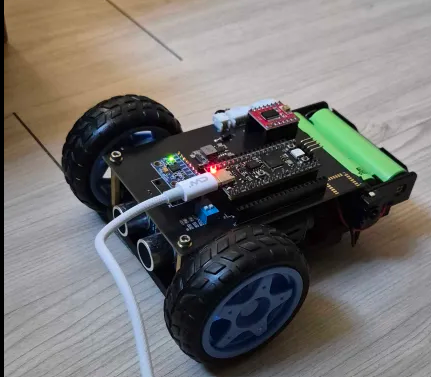
\includegraphics[width=0.6\textwidth]{Webcam/robot_test_filaire.png}
		\caption{IOT Car robot during the gesture-control tests over a wired link}
		\label{fig:robot-test-filaire}
	\end{figure}
	
	\subsection*{Real-time dashboard}
	
	A dashboard was added in order to visualise the robot's behaviour live.\\ The \texttt{parse\_status\_line()} function extracts, by regular expression, the position, angle, mode and distance values from the telemetry lines returned by the robot (Section~3.2).
	
	A first version displayed this dashboard in the same loop as the OpenCV capture, causing a low-level crash after a few tens of seconds (\texttt{Fatal Python error}, related to the GIL), a known conflict between OpenCV and matplotlib/Tkinter when they share the same process. The final version therefore moves the dashboard entirely into a \textbf{second process} (\texttt{multiprocessing.Process}), which communicates with the main process via a shared queue (\texttt{Queue}). The main process deposits a tuple (position, angle, mode, distance, elapsed time) there for each telemetry line received, which the dashboard process continuously empties, without ever sharing a graphical window with OpenCV.
	
	The dashboard displays three panels updated live:
	
	\newpage
	
	\begin{itemize}
		\item the robot's \textbf{trajectory}, with an arrow indicating its current orientation, recomputed at each update from the transmitted angle, and markers at the places where an obstacle was detected by the HC-SR04 (distance below 15~cm); a continuous obstacle is marked only once, at the first point where it is detected, to avoid accumulating redundant markers while it remains present;
		\item the change in the robot's \textbf{angle} over time;
		\item a \textbf{coloured timeline} of the mode history, reconstructed by grouping the telemetry lines into continuous segments of the same mode (forward in green, stop in grey, left turn in orange, right turn in blue).
	\end{itemize}
	
	\begin{figure}[H]
		\centering
		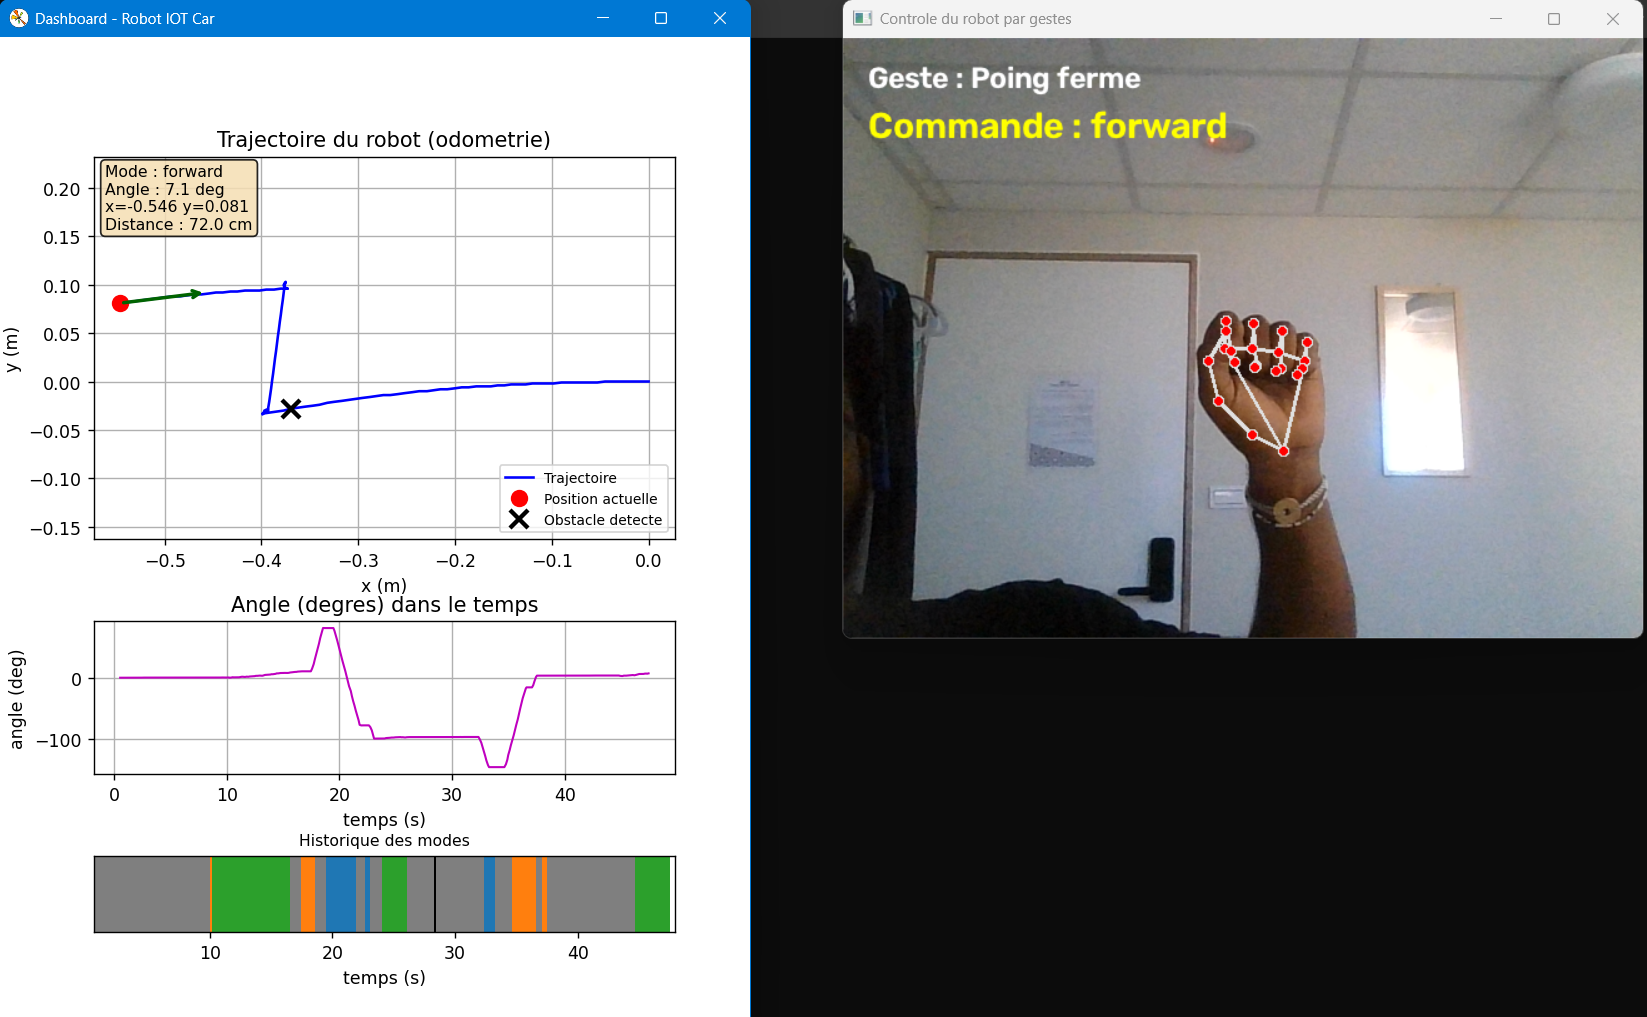
\includegraphics[width=\textwidth]{Webcam/dashboard_screenshot.png}
		\caption{Dashboard in operation, together with the gesture-control window}
		\label{fig:dashboard}
	\end{figure}
	
	\subsection*{Data export}
	
	At each telemetry line received, an instantaneous speed is computed from the Euclidean distance travelled between the current position and the previous one, divided by the time elapsed between the two measurements. All of the data (time, position, angle, mode, distance, speed) is accumulated in memory during the session, then exported when the program closes in two formats: a \textbf{CSV} file containing the raw data, and an \textbf{Excel} file containing the same data in a first tab, as well as an image of the dashboard (captured just before the second process closes) in a second tab.
	
	The file name is built from the current date and the total session duration (for example \texttt{session\_20260705\_2m22s.csv}), a numeric suffix being added automatically in the event of a collision with an already existing file.
	
	\subsection*{Benchmark results}
	
	%=================================================================================
	%	WEBCAM latency
	%=================================================================================
	
	\paragraph{Latency:} \mbox{} \\
	Latency was measured using a dedicated script (\texttt{benchmark\_latence.py}), structured in two successive phases.\\ 
	Phase~1 measures \textbf{segment A (vision)}: the \\ \texttt{mesurer\_segment\_vision()} function captures an image from the webcam, runs hand detection and gesture classification, then measures the total duration of this iteration using \texttt{time.perf\_counter()}, over 100 consecutive iterations (\texttt{N\_VISION}). \\
	Phase~2 measures \textbf{segment B+C (communication)}: the\\ \texttt{mesurer\_segment\_communication()} function restarts the robot with the same software sequence as the integration script (Section~4.1), then sends a \texttt{\{"ping": n\}} message according to the protocol defined in Section~3.2, and times the delay until the corresponding \texttt{\{"pong": n\}} is received, with a maximum wait of one second (\texttt{PING\_TIMEOUT}) beyond which the trial is counted as lost, over 100 exchanges (\texttt{N\_PINGPONG}).
	
	In both phases, the very first measurements are excluded from the final statistics (15 for vision, 5 for communication), the initialisation time of MediaPipe and TensorFlow on the first images not being representative of the steady state. The \texttt{calculer\_stats()} function then computes, for each segment, the mean, median, standard deviation, minimum and maximum using Python's \texttt{statistics} module, before export in CSV and Excel format.
	
	\begin{table}[H]
		\centering
		\small
		\begin{tabular}{lccccc}
			\toprule
			\textbf{Latency} & \textbf{Mean} & \textbf{Median} & \textbf{Std. dev.} & \textbf{Min} & \textbf{Max} \\
			\midrule
			Segment A (vision) & 26.37~ms & 25.90~ms & 4.88~ms & 22.01~ms & 59.67~ms \\
			Segment B+C (comm.) & 5.39~ms & 3.92~ms & 3.42~ms & 2.79~ms & 17.62~ms \\
			\bottomrule
		\end{tabular}
		\caption{Latency of the WebCam solution (85 and 83 measurements after warm-up)}
		\label{tab:latence-webcam}
	\end{table}
	
	\begin{figure}[H]
		\centering
		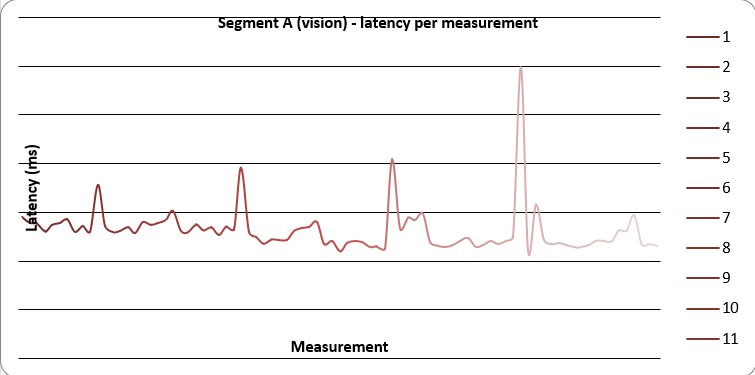
\includegraphics[width=0.8\textwidth]{Webcam/latence_vision_webcam.png}
		\caption{Latency per measurement for segment A (vision)}
		\label{fig:latence-vision-webcam}
	\end{figure}
	
	\begin{figure}[H]
		\centering
		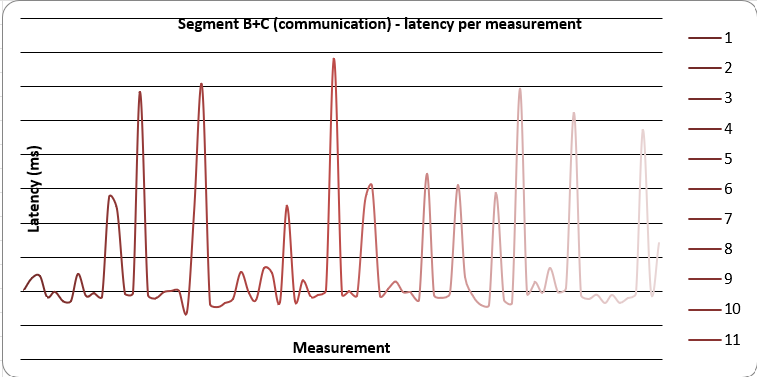
\includegraphics[width=0.8\textwidth]{Webcam/latence_comm_webcam.png}
		\caption{Latency per measurement for segment B+C (communication)}
		\label{fig:latence-comm-webcam}
	\end{figure}
	
	\paragraph{Analysis of the results:} \mbox{} \\
	The vision segment (median 25.90~ms) very largely dominates the communication segment (median 3.92~ms), the latency of the WebCam solution therefore coming mainly from the MediaPipe processing on the PC side, and not from the serial link to the robot. The total end-to-end software latency thus stands at around 30~ms in median, well below the human perceptibility threshold for a command delay, generally estimated between 100 and 150~ms.
	
	The two segments show occasional spikes, visible on the curves of Figures~\ref{fig:latence-vision-webcam} and~\ref{fig:latence-comm-webcam}. The communication segment shows a more concerning point: 12 pings out of 100 received no response within the allotted time, this loss not being evenly distributed but worsening progressively over the course of the session (2 losses after 30 sends, 6 after 60, 12 after 100). This drift suggests a progressive accumulation of some phenomenon on the robot side (for example a growing load related to the control loop or to CircuitPython memory management) rather than an occasional and random problem, a point that would deserve further investigation if time allows.
	
	%=================================================================================
	%	WEBCAM FPS
	%=================================================================================
	
	\paragraph{Throughput (FPS):} \mbox{} \\
	Throughput was measured using a dedicated script (\texttt{benchmark\_fps.py}), whose \texttt{mesurer\_fps()} function runs a continuous capture-and-classification loop for 30~seconds (\texttt{DUREE\_MESURE}), of which the first 3 seconds are excluded from the statistics (\texttt{WARMUP\_SEC}). At each iteration, the instantaneous FPS is computed as the inverse of the time elapsed since the previous iteration ($\text{FPS} = 1/\Delta t$), and each image is classified according to whether a hand was detected or not. The script thus accumulates, for each image, a tuple (elapsed time, instantaneous FPS, presence of a hand, warm-up indicator), from which three sets of statistics are computed separately: the overall throughput, the throughput with a hand detected, and the throughput without a hand detected.
	
	\begin{table}[H]
		\centering
		\small
		\begin{tabular}{lccccc}
			\toprule
			\textbf{Throughput} & \textbf{Mean} & \textbf{Median} & \textbf{Std. dev.} & \textbf{Min} & \textbf{Max} \\
			\midrule
			Overall (811 images) & 30.61~FPS & 31.62~FPS & 3.63 & 12.21~FPS & 37.33~FPS \\
			With hand (766 images) & 30.62~FPS & 31.65~FPS & 3.66 & 12.21~FPS & 37.33~FPS \\
			Without hand (45 images) & 30.57~FPS & 31.15~FPS & 3.19 & 21.52~FPS & 34.86~FPS \\
			\bottomrule
		\end{tabular}
		\caption{Throughput (FPS) of the WebCam solution (30~s measurement, warm-up excluded)}
		\label{tab:fps-webcam}
	\end{table}
	
	\begin{figure}[H]
		\centering
		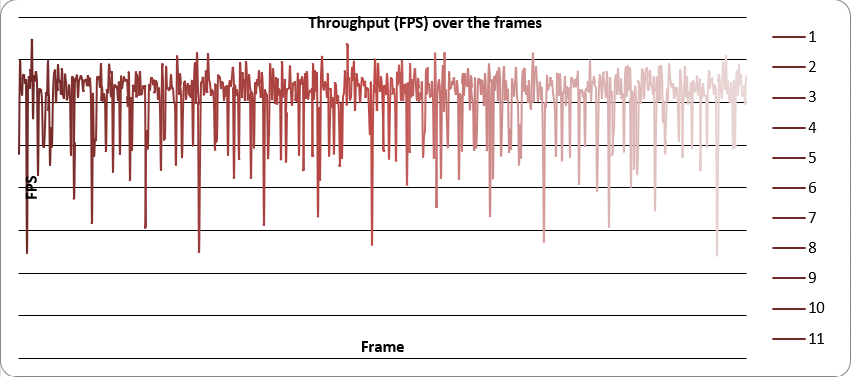
\includegraphics[width=0.8\textwidth]{Webcam/fps_webcam.png}
		\caption{Throughput (FPS) of the WebCam solution over the images}
		\label{fig:fps-webcam}
	\end{figure}
	
	\paragraph{Analysis of the results:} \mbox{} \\
	The mean throughput stands at around 30.6~frames per second, which corresponds to the classic limit of a standard webcam clocked at 30~FPS: the processing pipeline (capture, MediaPipe, classification) is therefore fast enough not to be the limiting factor, it is the camera that sets the pace. A notable result: the throughput is almost identical with a hand detected (30.62~FPS) and without a hand (30.57~FPS), the presence of a gesture to track therefore not appreciably increasing the processing load.
	
	The curve in Figure~\ref{fig:fps-webcam} shows several occasional drops, down to a minimum of 12.21~FPS, spread irregularly over the whole measurement duration rather than concentrated at a single moment. These drops probably correspond to variations in system load (other PC processes) rather than to a phenomenon related to MediaPipe itself. The moderate standard deviation (3.63, i.e. about 12\% of the mean) nevertheless reflects an overall stable throughput.
	
	%=================================================================================
	%	WEBCAM recognition reliability
	%=================================================================================
	
	\paragraph{Recognition reliability:} \mbox{} \\
	Reliability was measured using a dedicated script (\texttt{benchmark\_fiabilite.py}), following a manual protocol: the \texttt{acquerir\_essais()} function displays live the gesture detected by the system, and the user indicates, by pressing a key (1 to 4), the gesture they actually intended to make; the script then records the pair (intended gesture, detected gesture) at the precise moment of this key press. Acquisition stops automatically once each of the four gestures has reached 20 trials (\texttt{N\_PAR\_GESTE}), i.e. 80 trials in total. The \texttt{construire\_matrice()} function then aggregates all of the trials into a confusion matrix (one row per intended gesture, one column per detected gesture, plus a ``not detected'' column), exported to Excel with a colour code (diagonal in green for correct trials, off-diagonal cells in red in the event of an error).
	
	\begin{table}[H]
		\centering
		\small
		\begin{tabular}{lccccc}
			\toprule
			\textbf{Intended \textbackslash\ Detected} & \textbf{Forward} & \textbf{Stop} & \textbf{Left} & \textbf{Right} & \textbf{Not detected} \\
			\midrule
			Forward & 20 & 0 & 0 & 0 & 0 \\
			Stop & 0 & 20 & 0 & 0 & 0 \\
			Left & 0 & 0 & 20 & 0 & 0 \\
			Right & 0 & 0 & 0 & 20 & 0 \\
			\bottomrule
		\end{tabular}
		\caption{Confusion matrix of the WebCam solution (80 trials, 20 per gesture)}
		\label{tab:confusion-webcam}
	\end{table}
	
	\begin{figure}[H]
		\centering
		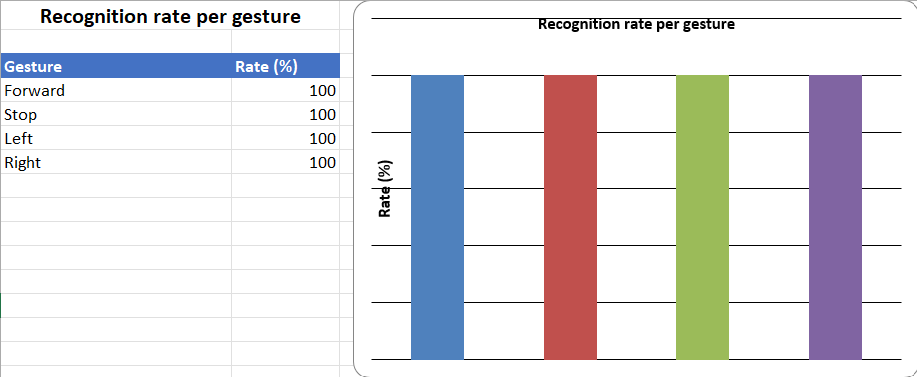
\includegraphics[width=0.7\textwidth]{Webcam/fiabilite_webcam.png}
		\caption{Recognition rate per gesture (WebCam solution)}
		\label{fig:fiabilite-webcam}
	\end{figure}
	
	\paragraph{Analysis of the results:} \mbox{} \\
	The WebCam solution achieves perfect reliability: the confusion matrix is a full diagonal, with no confusion between gestures and no non-detection, i.e. an overall recognition rate of 100\% (80/80). This result is explained by the robustness of the MediaPipe model, which provides precise hand landmarks, combined with a classification logic based on finger states that is clearly separated between the four chosen gestures. These gestures were, moreover, deliberately selected to be visually well distinct from one another, which strongly limits the risk of confusion. This rate constitutes an upper reference for the comparison with the solutions studied in the following sections.
	
	%=================================================================================
	%	WEBCAM consumption
	%=================================================================================
	
	\paragraph{Power consumption:} \mbox{} \\
	This last metric aimed to measure the electrical consumption of the webcam and of the RP2040 using an INA219 module, placed in series on the power supply of each component, in order to compare the camera and the robot at rest and in active operation. This measurement would have made it possible to answer a question complementary to the three previous metrics: beyond the speed and reliability of a solution, what is its potential battery autonomy, a decisive criterion for a real embedded application, where the robot would no longer be continuously powered by a PC. It would also have made it possible to highlight a trade-off specific to the WebCam solution: while offloading the processing to a PC relieves the RP2040's load, it in fact shifts the consumption onto a machine far more power-hungry than a microcontroller, an energy cost that is invisible if only the camera and the robot are measured in isolation.
	
	This measurement could ultimately not be carried out, for a reason that is methodological rather than technical: inserting an INA219 module on the power supply of a component requires temporarily cutting an existing power wire, in order to insert the sensor in series on the circuit. However, all of the hardware used for this project (webcam, smart cameras, IOT Car robot) belongs to the laboratory and was lent as part of the internship, without such a structural modification of the wiring having been explicitly authorised. Out of caution regarding hardware that is not mine, this measurement was therefore deliberately set aside for all of the solutions studied, rather than risked on a single component. This methodological limitation, documented here for the WebCam solution, applies in the same way to the four other solutions of the benchmark.
	
	\newpage
	
	%----------------------------------------------------------------------
	%	5.4 OpenMV
	%----------------------------------------------------------------------
	
	\section{OpenMV}
	\label{sec:openmv-limitation}
	
	This section presents the integration of the OpenMV smart camera and the hardware blockage encountered during deployment, which prevented the full benchmark from being carried out for this solution.
	
	\subsection*{Principle and architecture}
	
	The camera used is an OpenMV3 R1 (OV7725-M7 module), embedding an STM32F765 microcontroller with no dedicated hardware accelerator for neural-network inference (NPU), presented in the technical overview in Section~2.2.2. The processing intelligence is meant to be entirely embedded in the camera: a custom TinyML model, trained with Edge Impulse, must recognise the four gestures and transmit the result to the PC over its USB port, on a port distinct from that of the robot. The PC then acts as a simple relay, forwarding the already-computed command to the RP2040 over its own USB port, without performing any vision processing itself, according to the protocol established in Section~3.2.
	
	\subsection*{Training the model with Edge Impulse}
	
	The model was designed and trained on the Edge Impulse platform, structured as an \textit{impulse}: a processing chain that takes raw data as input, extracts features from it, then classifies them using a learning block. The impulse built for this solution comprises an image-data block (resized to 64$\times$64 pixels), an image-processing block, and a classification block with four outputs corresponding to the four gestures of the project (Forward, Right, Left, Stop).
	
	\begin{figure}[H]
		\centering
		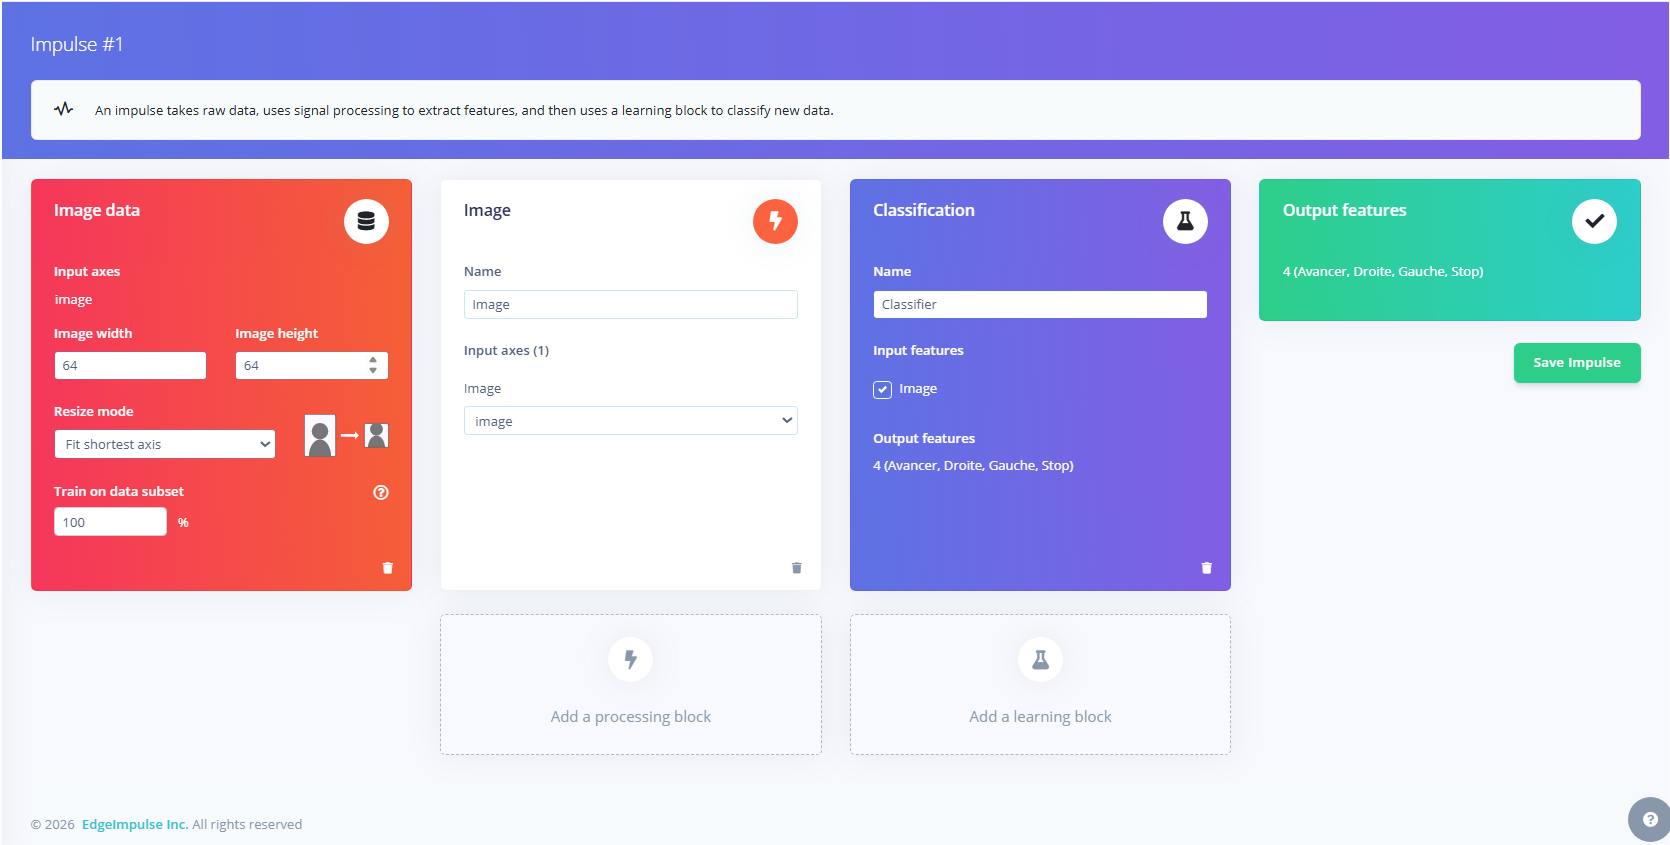
\includegraphics[width=\textwidth]{OpenMV/create_impulse.png}
		\caption{Structure of the Edge Impulse impulse (64$\times$64 image data, classification with 4 outputs)}
		\label{fig:openmv-impulse}
	\end{figure}
	
	The dataset was built directly from the camera, with 282 images spread across four classes, automatically split into a training set (82\%, 231 images) and a test set (18\%, 51 images).
	
	\begin{figure}[H]
		\centering
		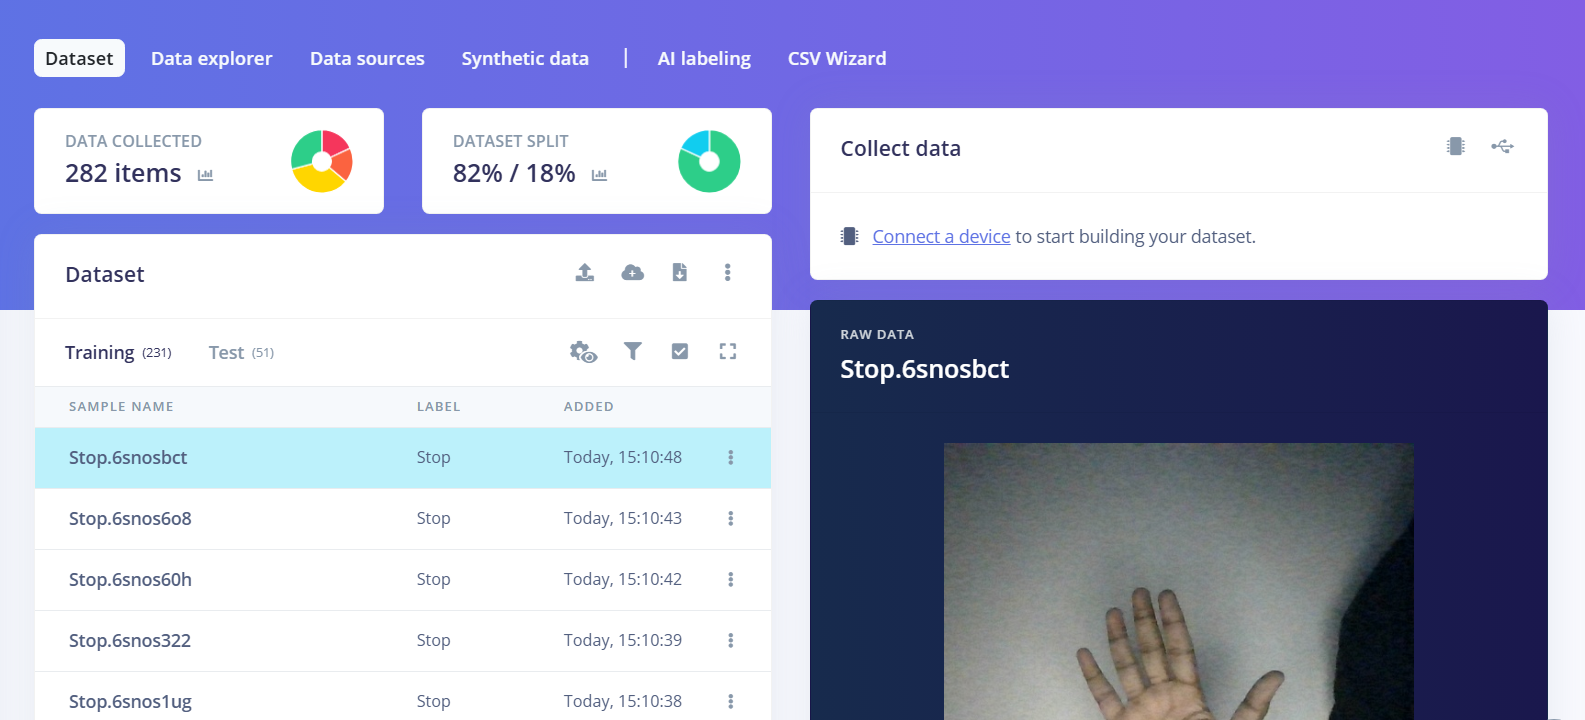
\includegraphics[width=\textwidth]{OpenMV/Data_Acquisition.png}
		\caption{Dataset collected in Edge Impulse (282 images, 4 classes)}
		\label{fig:openmv-dataset}
	\end{figure}
	
	The training of the neural network was set up with 30 training cycles, a learning rate of 0.0005, a batch size of 32, and int8-quantised model profiling (enabled to obtain an estimate of the RAM and flash needed on the embedded target).
	
	\begin{figure}[H]
		\centering
		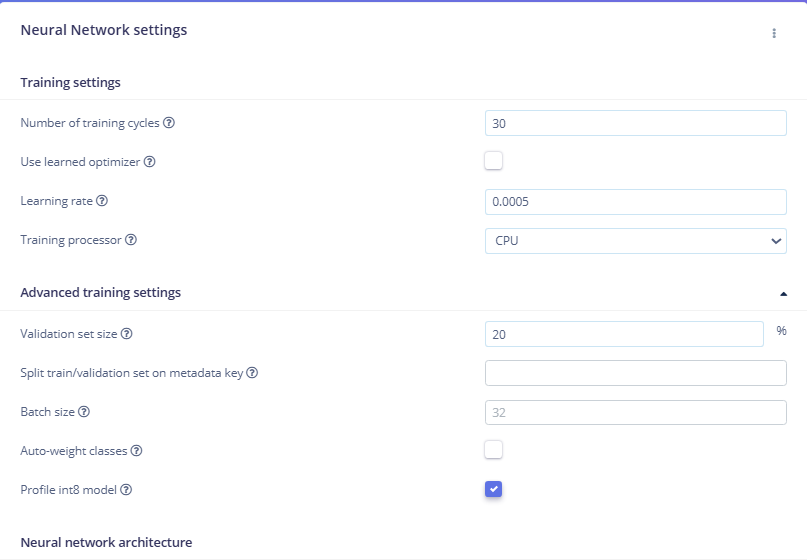
\includegraphics[width=0.85\textwidth]{OpenMV/train_parameters.png}
		\caption{Training parameters of the neural network}
		\label{fig:openmv-train-params}
	\end{figure}
	
	The model obtained after this first training (64$\times$64 resolution, TensorFlow Lite engine) reaches an accuracy of 95.7\% on the validation set, with an almost perfect confusion matrix (residual confusion only between the Right and Left gestures). The embedded-performance estimate provided by Edge Impulse reports an inference time of 12~ms, a peak memory usage of 82.7~KB and a flash size of 65.9~KB, values that are a priori compatible with the camera's 512~KB of RAM.
	
	\begin{figure}[H]
		\centering
		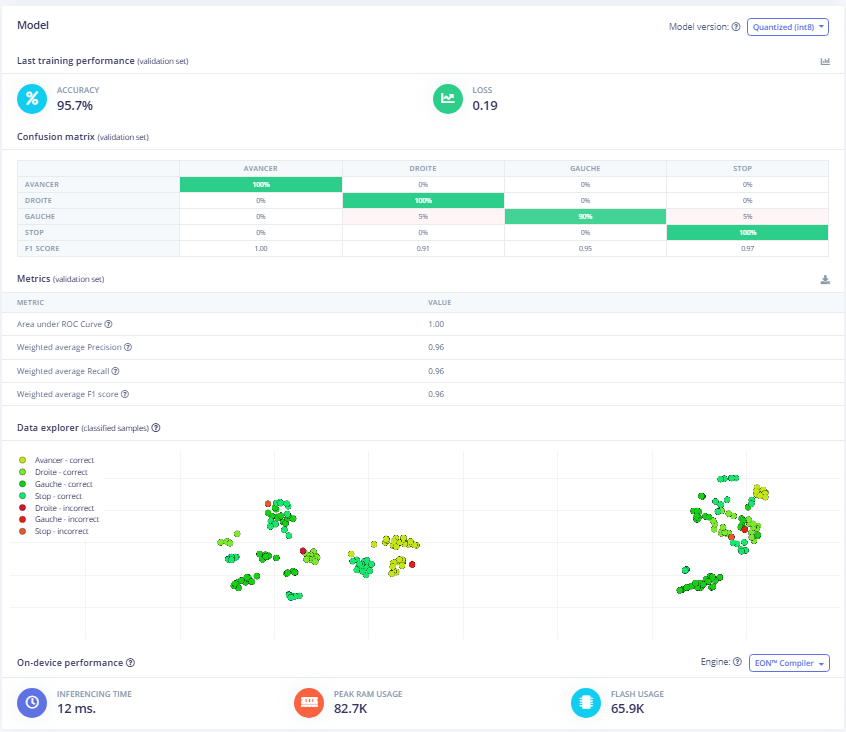
\includegraphics[width=\textwidth]{OpenMV/train_result.png}
		\caption{Training results (95.7\% accuracy, confusion matrix, embedded-performance estimate)}
		\label{fig:openmv-train-result}
	\end{figure}
	
	Several iterations were then needed to try to make the model actually fit on the camera, by progressively reducing the input resolution and changing the inference engine, summarised in Table~\ref{tab:openmv-iterations}.
	
	\begin{table}[H]
		\centering
		\small
		\begin{tabular}{lccccl}
			\toprule
			\textbf{Resolution} & \textbf{Engine} & \textbf{Accuracy} & \textbf{Est. RAM} & \textbf{Flash} & \textbf{Result} \\
			\midrule
			64$\times$64 & TensorFlow Lite & 95.7\% & 82.7~KB & 65.9~KB & Failure (allocation) \\
			48$\times$48 & TensorFlow Lite & 85.1\% & 31.1~KB & 59.1~KB & Failure (allocation) \\
			32$\times$32 (light CNN) & EON Compiler & 42.3\% & 22.7~KB & 41.9~KB & Failure (allocation) \\
			\bottomrule
		\end{tabular}
		\caption{Optimisation iterations of the OpenMV model}
		\label{tab:openmv-iterations}
	\end{table}
	
	Despite a reduction of the estimated RAM by a factor of more than 3.5 between the first and the last iteration, and a significant loss of accuracy in return, none of these configurations allowed the model to be functionally deployed on the camera.
	
	\subsection*{Blockage encountered during deployment}
	
	With the first model (64$\times$64), loading failed with the error \texttt{Failed to allocate tensors}, consistent with insufficient RAM for the memory space needed for inference. Reducing the resolution (64$\times$64 to 48$\times$48) made this initial message disappear, but a different and systematic error then appeared: \texttt{MemoryError, memory allocation failed, allocating 4080 bytes}. Unlike the first symptom, this error concerns a small, fixed-size allocation (4080 bytes), and not the whole model.
	
	To isolate the cause of this residual blockage, several actions were carried out one after another, each with no effect on the error:
	
	\begin{itemize}
		\item reducing the resolution down to 32$\times$32 and replacing the \textit{transfer learning} model with a lighter custom CNN (two convolution layers, 16 then 32 filters);
		\item switching the inference engine from TensorFlow Lite to the EON Compiler, bringing the estimated RAM down to 22.7~KB;
		\item correcting a code inconsistency (a requested capture window of 240$\times$240 while the sensor was configured in QQVGA, i.e. 160$\times$120);
		\item loading the model before initialising the camera, to rule out a hypothesis of memory fragmentation related to the sensor;
		\item testing the loading of the model without any camera initialisation, reproducing the error identically with 47.7~KB of free RAM available;
		\item a complete update of the camera firmware to the latest development version available.
	\end{itemize}
	
	The 4080-byte allocation error reproduced itself identically across all of these configurations, including after the complete firmware update. This invariance, combined with the large gap between the measured free RAM (46 to 48~KB) and the size of the failing allocation, indicates that the blockage is neither a model-size problem nor a bug fixable by a software update, but very probably a hardware limitation specific to this camera model. The OpenMV3~R1 (OV7725-M7, STM32F765) is an old board, lacking an NPU and external RAM, unlike the more recent models of the OpenMV range for which support for embedded inference is actively developed and tested.
	
	\subsection*{Benchmark results}
	
	The blockage described above prevents the model from running on the camera, and therefore the measurement of the four metrics under the same conditions as for the other solutions.
	
	\begin{table}[H]
		\centering
		\small
		\begin{tabular}{lcccc}
			\toprule
			\textbf{OpenMV latency} & \textbf{Mean} & \textbf{Std. dev.} & \textbf{Min} & \textbf{Max} \\
			\midrule
			\multicolumn{5}{c}{Not measurable, hardware blockage described above} \\
			\bottomrule
		\end{tabular}
		\caption{Latency of the OpenMV solution, not measurable}
	\end{table}
	
	\begin{table}[H]
		\centering
		\small
		\begin{tabular}{lc}
			\toprule
			\textbf{OpenMV throughput} & \textbf{FPS} \\
			\midrule
			Not measurable, hardware blockage described above & - \\
			\bottomrule
		\end{tabular}
		\caption{Throughput of the OpenMV solution, not measurable}
	\end{table}
	
	\begin{table}[H]
		\centering
		\small
		\begin{tabular}{l|cccc|c}
			\toprule
			\textbf{Intended \textbackslash\ Detected} & \textbf{Forward} & \textbf{Stop} & \textbf{Left} & \textbf{Right} & \textbf{Not detected} \\
			\midrule
			\multicolumn{6}{c}{Not measurable, hardware blockage described above} \\
			\bottomrule
		\end{tabular}
		\caption{Confusion matrix of the OpenMV solution, not measurable}
	\end{table}
	
	\begin{table}[H]
		\centering
		\small
		\begin{tabular}{lcc}
			\toprule
			\textbf{OpenMV consumption} & \textbf{At rest} & \textbf{Active} \\
			\midrule
			Camera & \multicolumn{2}{c}{Not measurable, hardware blockage described above} \\
			\bottomrule
		\end{tabular}
		\caption{Consumption of the OpenMV solution, not measurable}
	\end{table}
	
	Although incomplete from the point of view of the four metrics, this blockage constitutes in itself a relevant result with respect to the problem posed in Section~1.2: it demonstrates that the choice of the precise hardware of a smart camera, and not only of its general category, directly conditions the feasibility of an embedded processing architecture, independently of the quality of the trained model.
	
	\newpage
	
	%----------------------------------------------------------------------
	%	5.5 Nicla Vision
	%----------------------------------------------------------------------
	
	\section{Nicla Vision}
	
	\subsection*{Principle}
	
	Unlike the OpenMV Cam M7, whose datasheet and hardware limitations are detailed in Section~2.2.2, the Nicla Vision embeds a more powerful microcontroller (STM32H747, dual-core, 1~MB of RAM) presented in Section~2.2.3, and shares the same programming environment as OpenMV (MicroPython firmware, OpenMV IDE). The objective remains the same: recognise the four gestures using a TinyML model trained with Edge Impulse, run entirely on the camera, and transmit the result to the PC, which acts as a simple relay to the robot.
	
	\subsection*{Building the dataset}
	
	The images were captured directly from the camera, using a dedicated script run in the OpenMV IDE, which saves a stream of images into one folder per class. A first set of 160 images was thus built, split into a training set (80\%) and a test set (20\%).
	
	\begin{figure}[H]
		\centering
		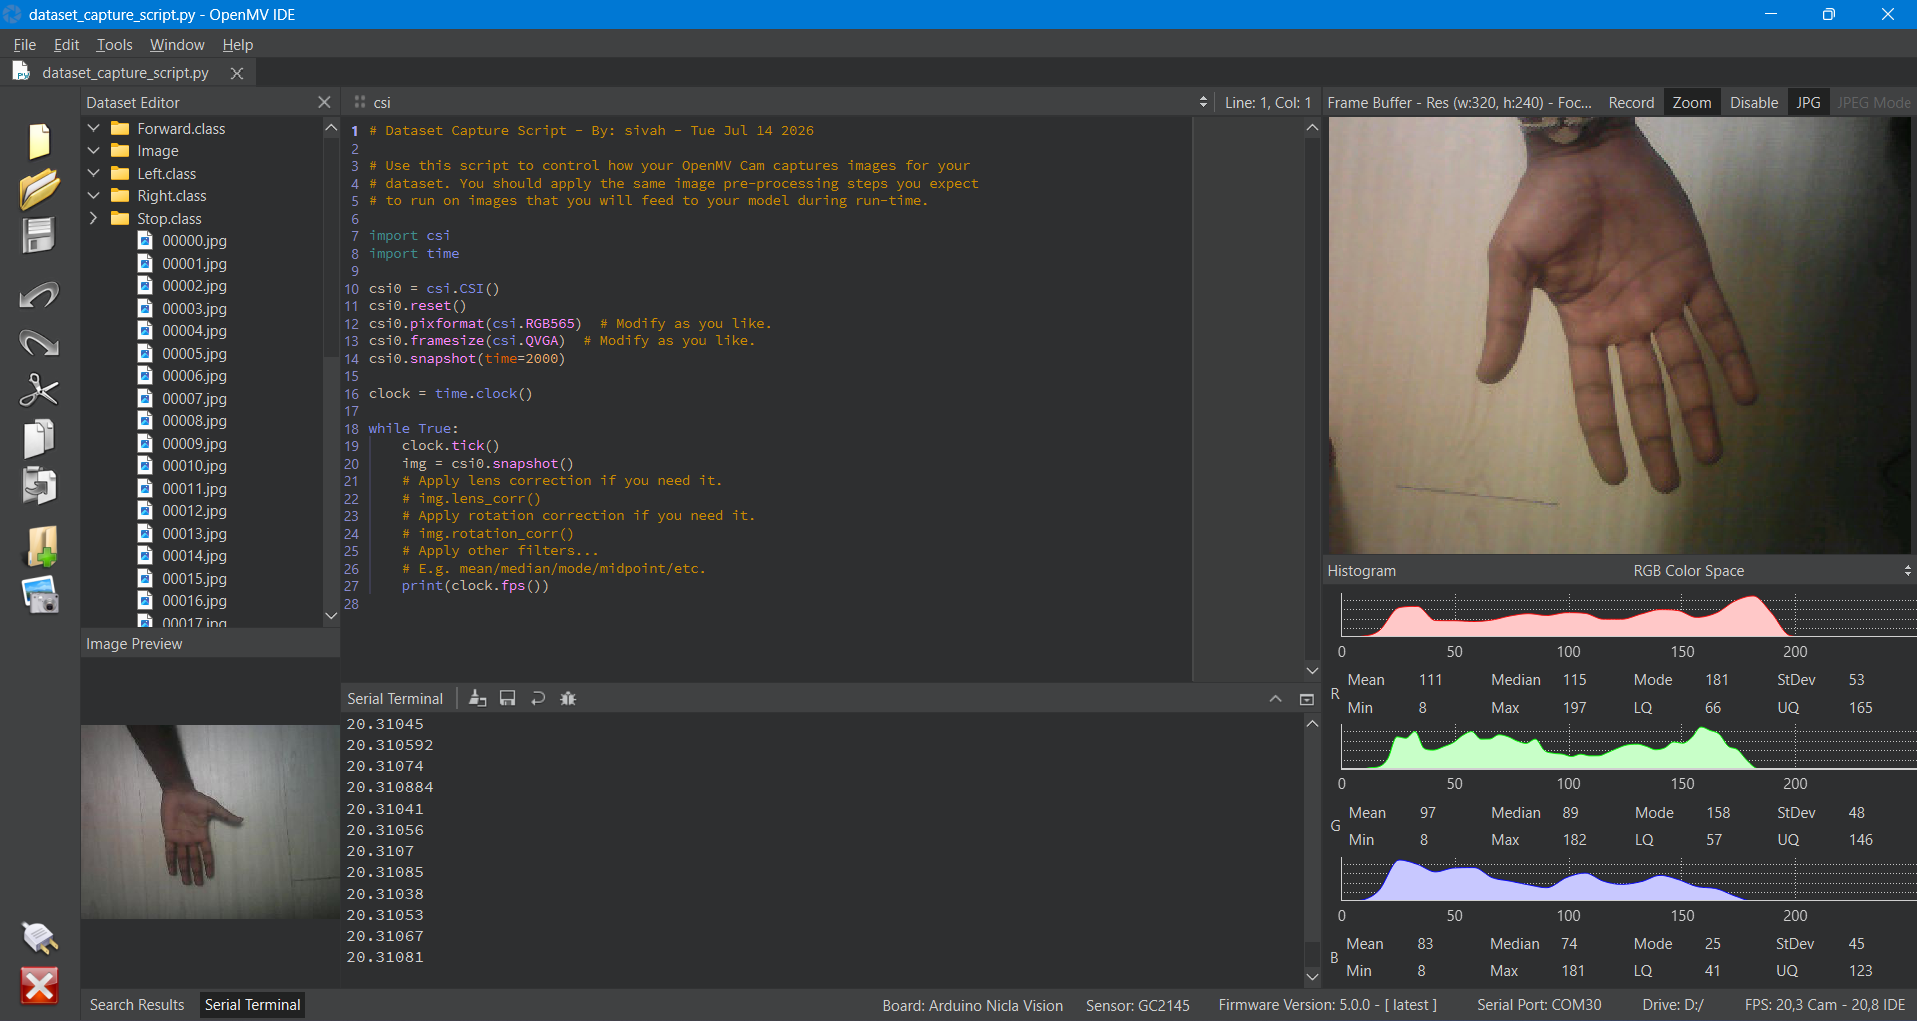
\includegraphics[width=\textwidth]{NiclaVision/Capture.png}
		\caption{Dataset-capture script run in the OpenMV IDE on the Nicla Vision}
		\label{fig:nicla-capture-script}
	\end{figure}
	
	\begin{figure}[H]
		\centering
		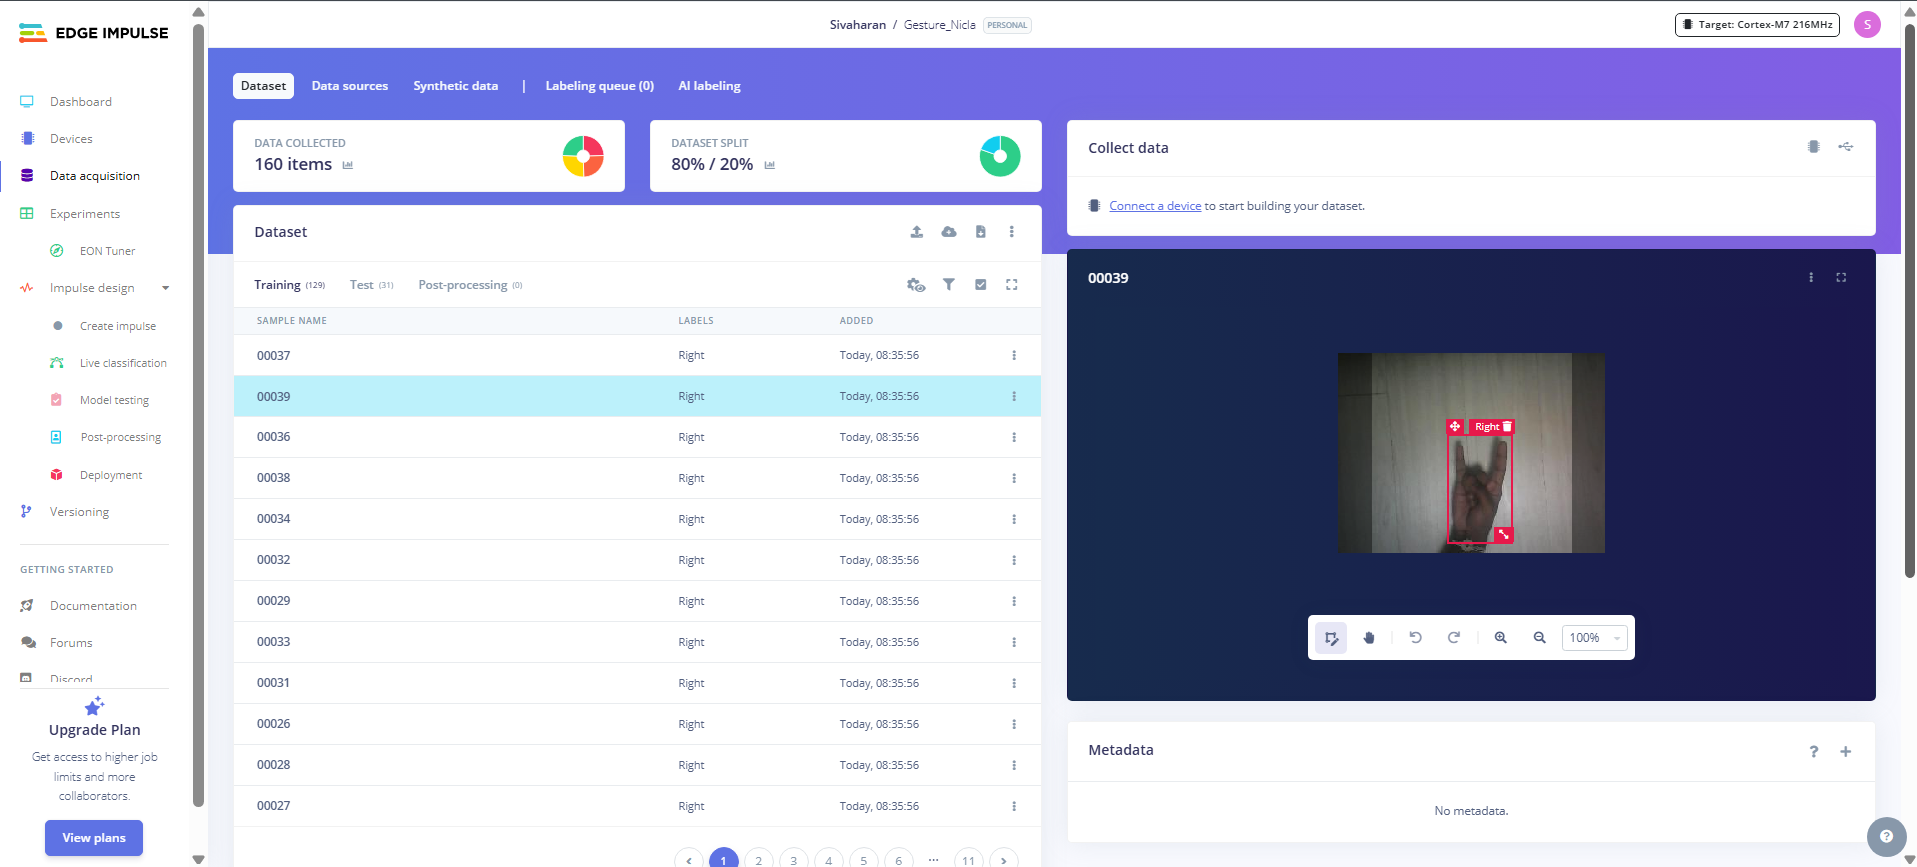
\includegraphics[width=\textwidth]{NiclaVision/Donne.png}
		\caption{Dataset collected in Edge Impulse (160 images, 80/20 split)}
		\label{fig:nicla-dataset}
	\end{figure}
	
	Each image was then labelled manually, by drawing a bounding box around the gesture concerned and assigning it its class.
	
	\begin{figure}[H]
		\centering
		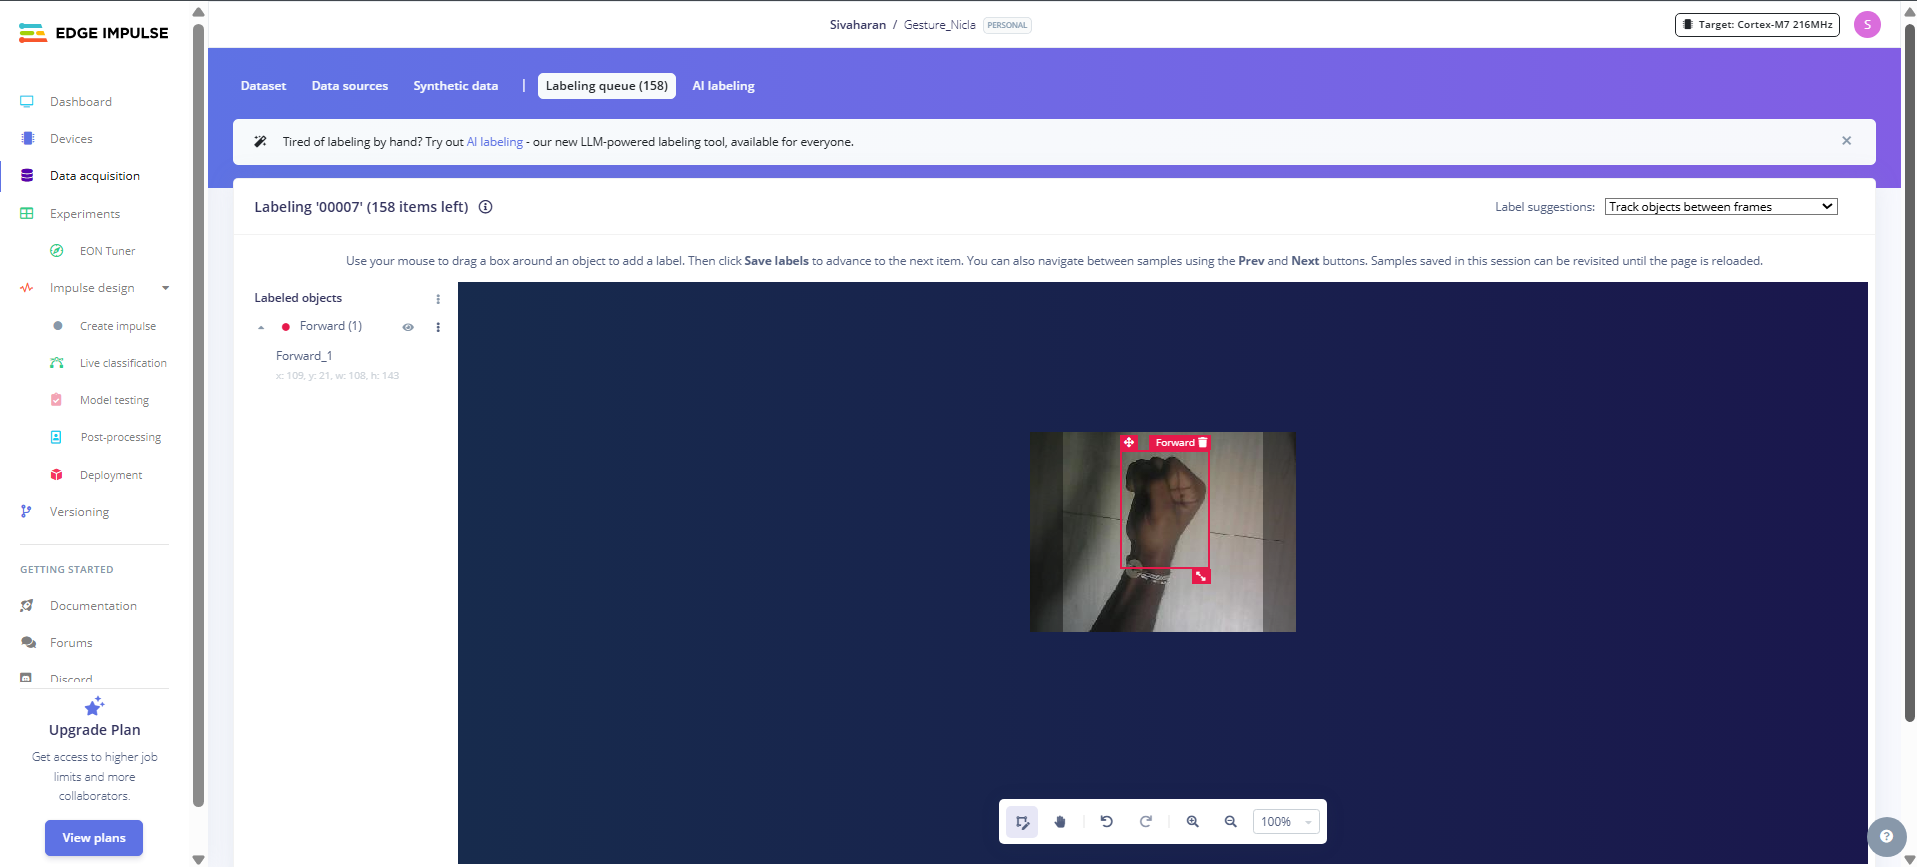
\includegraphics[width=\textwidth]{NiclaVision/Etiquettage.png}
		\caption{Manual labelling of the images by bounding box in Edge Impulse}
		\label{fig:nicla-etiquetage}
	\end{figure}
	
	\subsection*{Design of the impulse}
	
	Unlike the first attempt on the OpenMV M7 (Section~4.2), which used a simple image-classification approach, the impulse built for the Nicla Vision relies on an \textbf{object-detection} approach, better suited to locating a gesture within the image. The images are resized to 96$\times$96 pixels, a resolution higher than the one that had caused problems on the OpenMV M7, made possible by the larger RAM of the Nicla Vision.
	
	\begin{figure}[H]
		\centering
		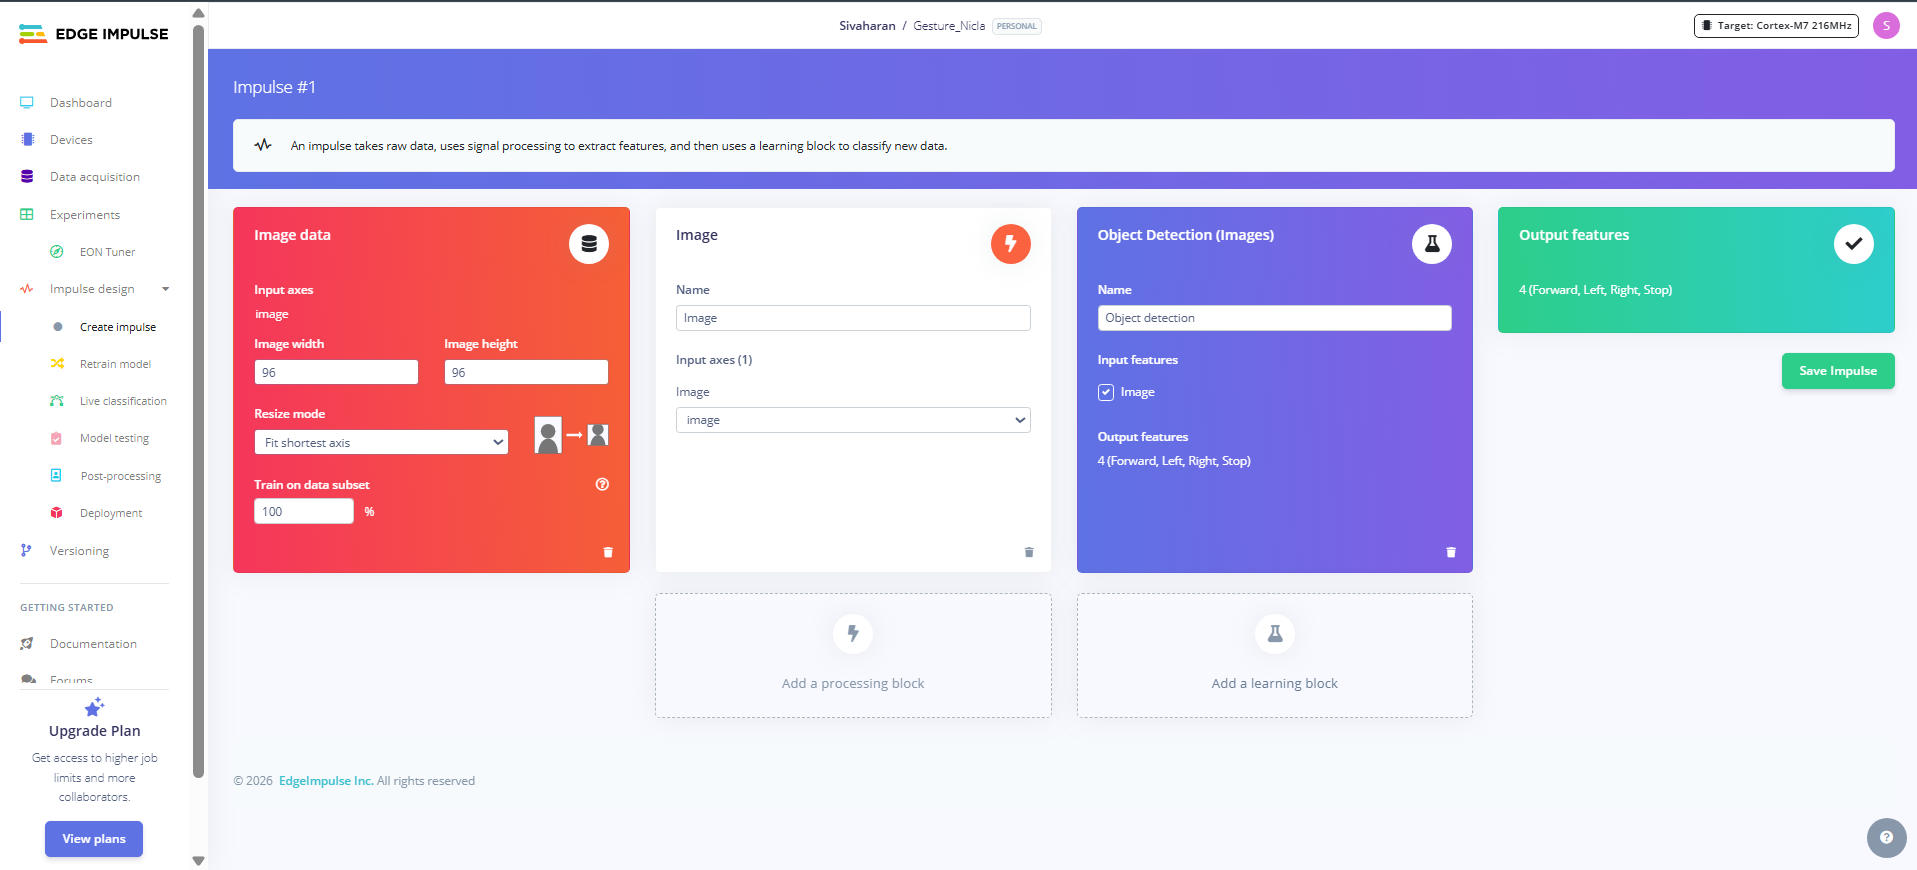
\includegraphics[width=\textwidth]{NiclaVision/Impulse_parameters.png}
		\caption{Structure of the impulse (96$\times$96 image data, object-detection block, 4 output classes)}
		\label{fig:nicla-impulse}
	\end{figure}
	
	\begin{figure}[H]
		\centering
		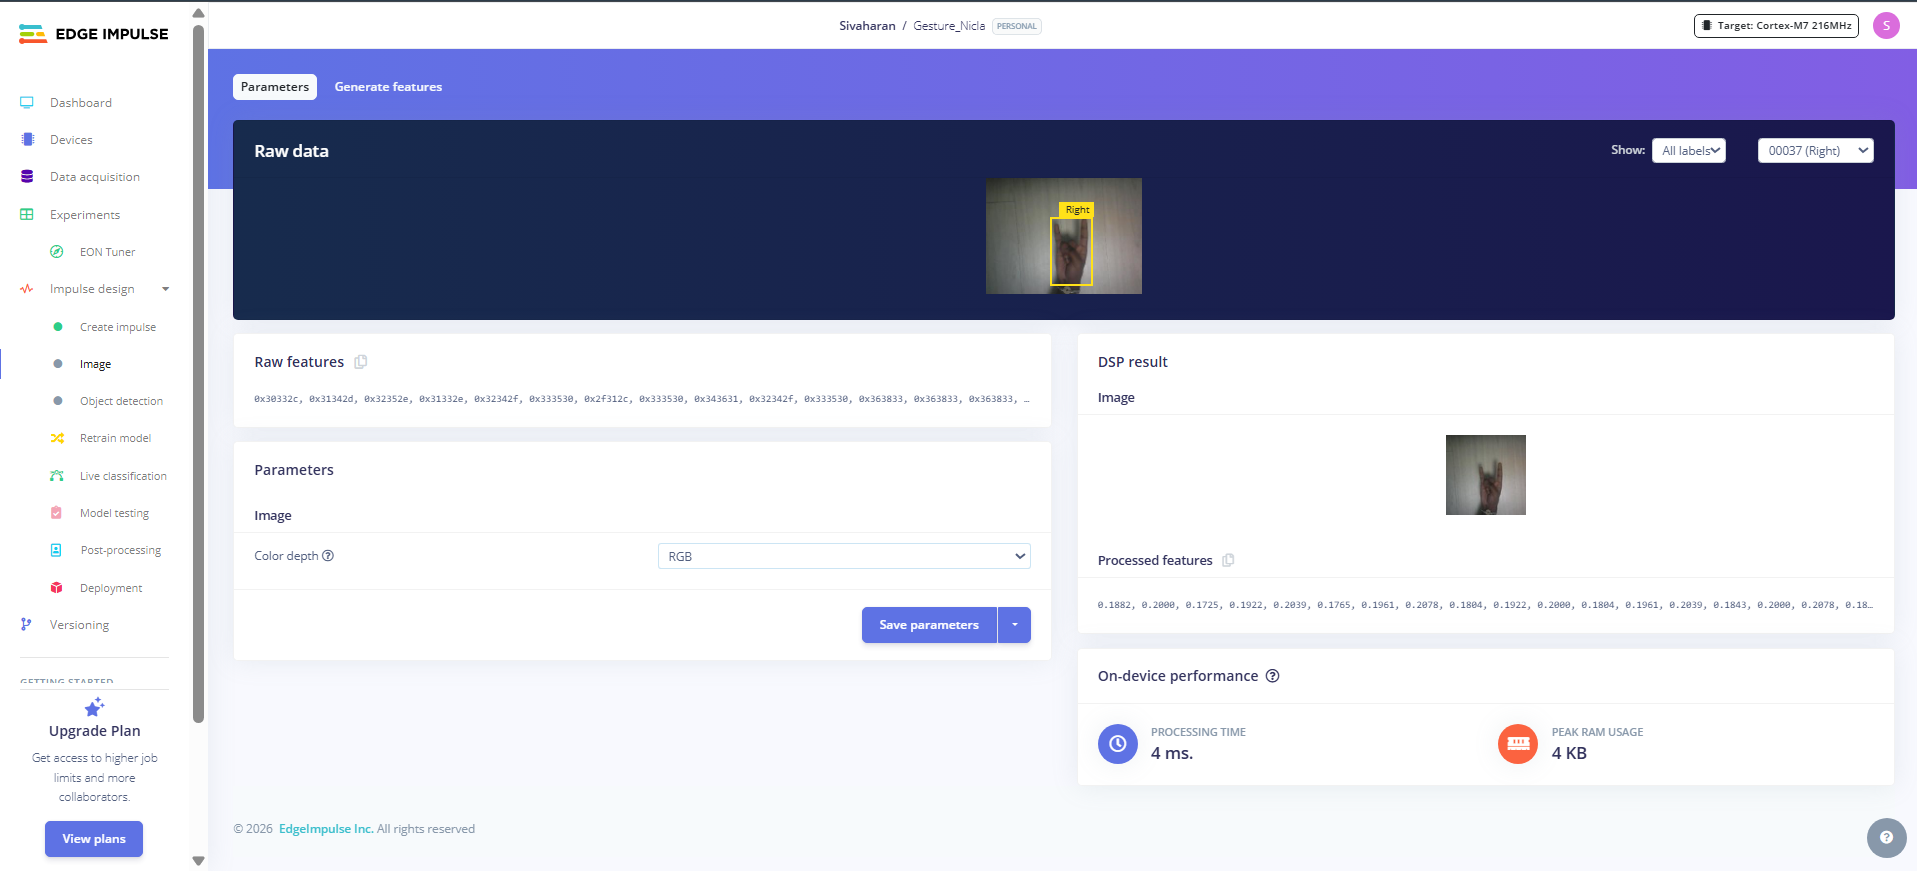
\includegraphics[width=0.85\textwidth]{NiclaVision/Image_parameters.png}
		\caption{Parameters of the image-processing block (RGB colour depth)}
		\label{fig:nicla-image-params}
	\end{figure}
	
	\subsection*{Feature generation}
	
	Once the impulse is defined, Edge Impulse generates the features from the 129 images of the training set, spread across the four classes. The resulting point cloud (\textit{feature explorer}) shows a relatively clear separation between the classes, with, however, a certain overlap between the Forward and Stop gestures.
	
	\begin{figure}[H]
		\centering
		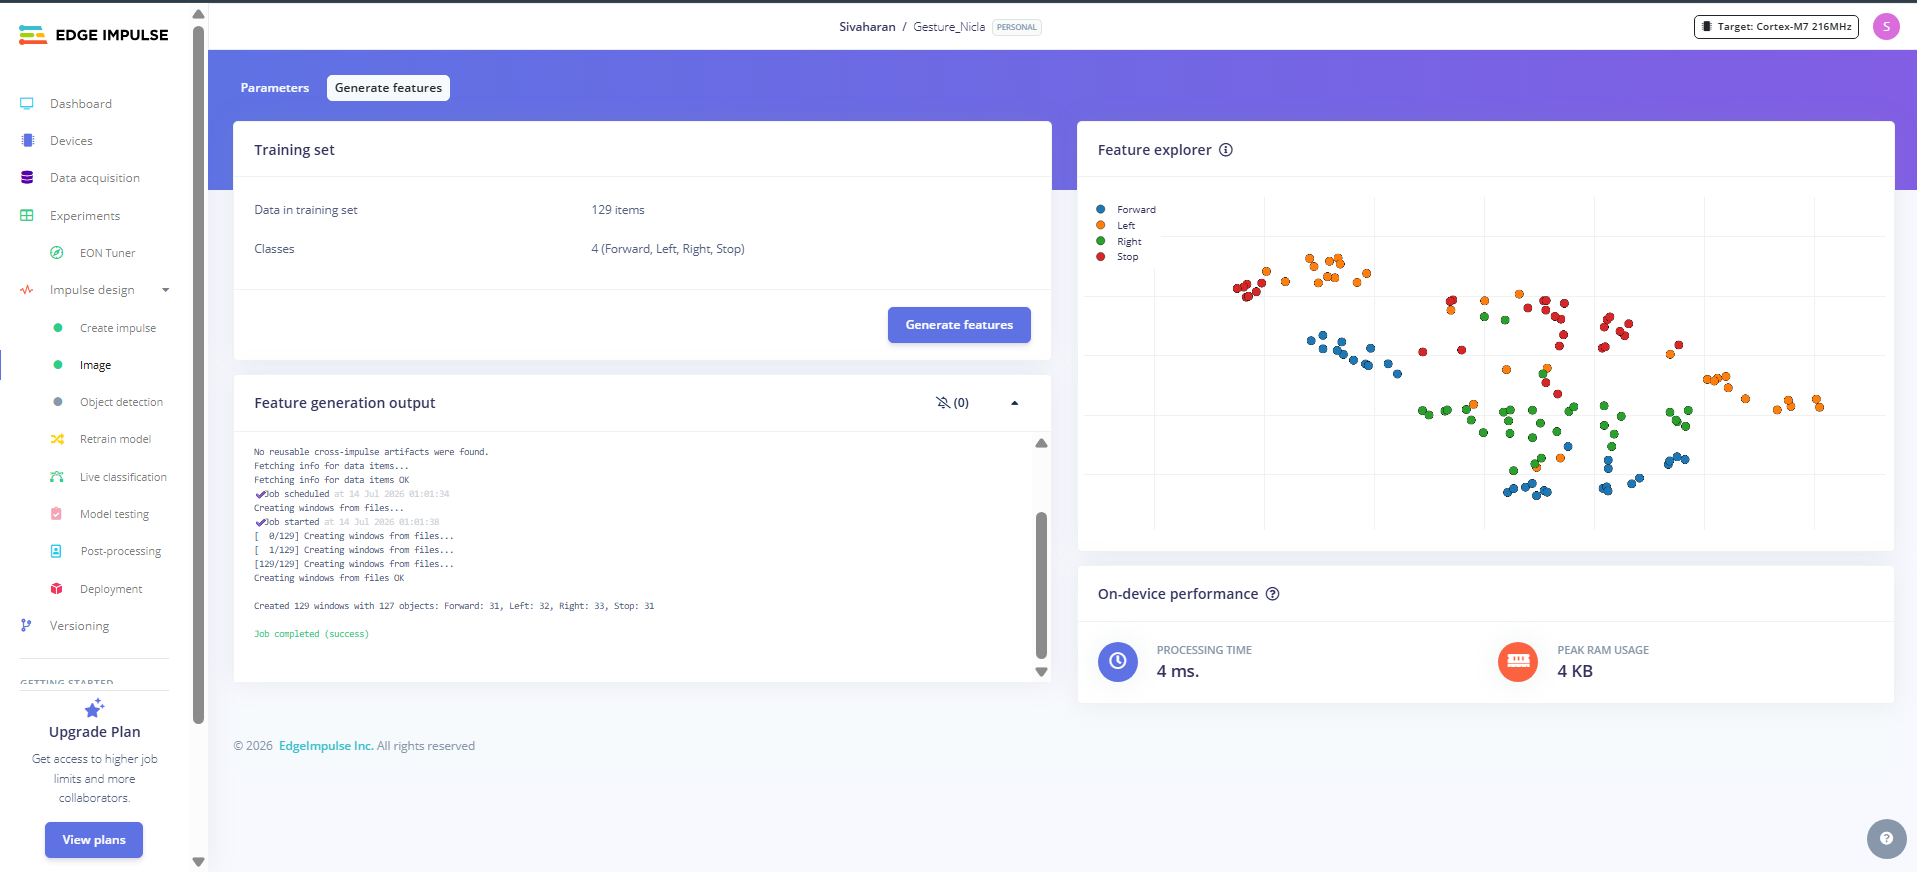
\includegraphics[width=\textwidth]{NiclaVision/Feature_generated.png}
		\caption{Feature generation (129 images, 4 classes) and visualisation in the \textit{feature explorer}}
		\label{fig:nicla-features-generated}
	\end{figure}
	
	\begin{figure}[H]
		\centering
		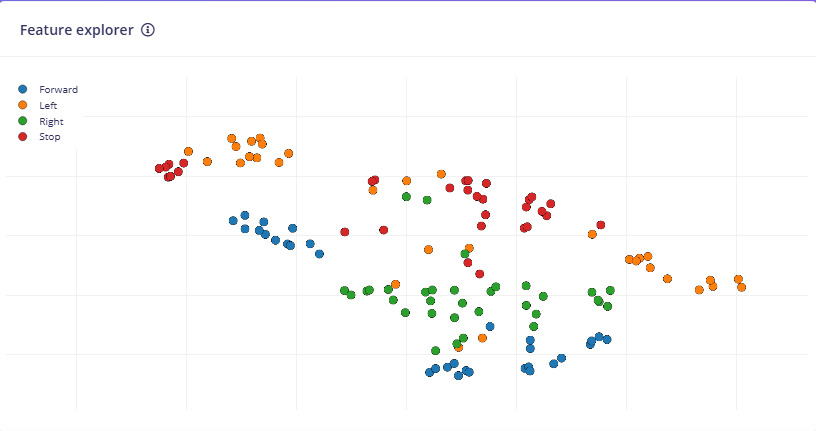
\includegraphics[width=0.75\textwidth]{NiclaVision/Feature_data_for_report.png}
		\caption{Detail of the features extracted for one sample (raw image, DSP features)}
		\label{fig:nicla-feature-data}
	\end{figure}
	
	At this stage, Edge Impulse already provides a first embedded-performance estimate for the DSP processing alone (excluding the neural network): about 4~ms and 4~KB of RAM, a value markedly lower than that of the complete model presented later.
	
	\subsection*{Training the model}
	
	The neural network used is a FOMO (\textit{Faster Objects, More Objects}) architecture based on MobileNetV2 (width~0.35), trained over 70 cycles with a learning rate of 0.01 and data augmentation enabled.
	
	\begin{figure}[H]
		\centering
		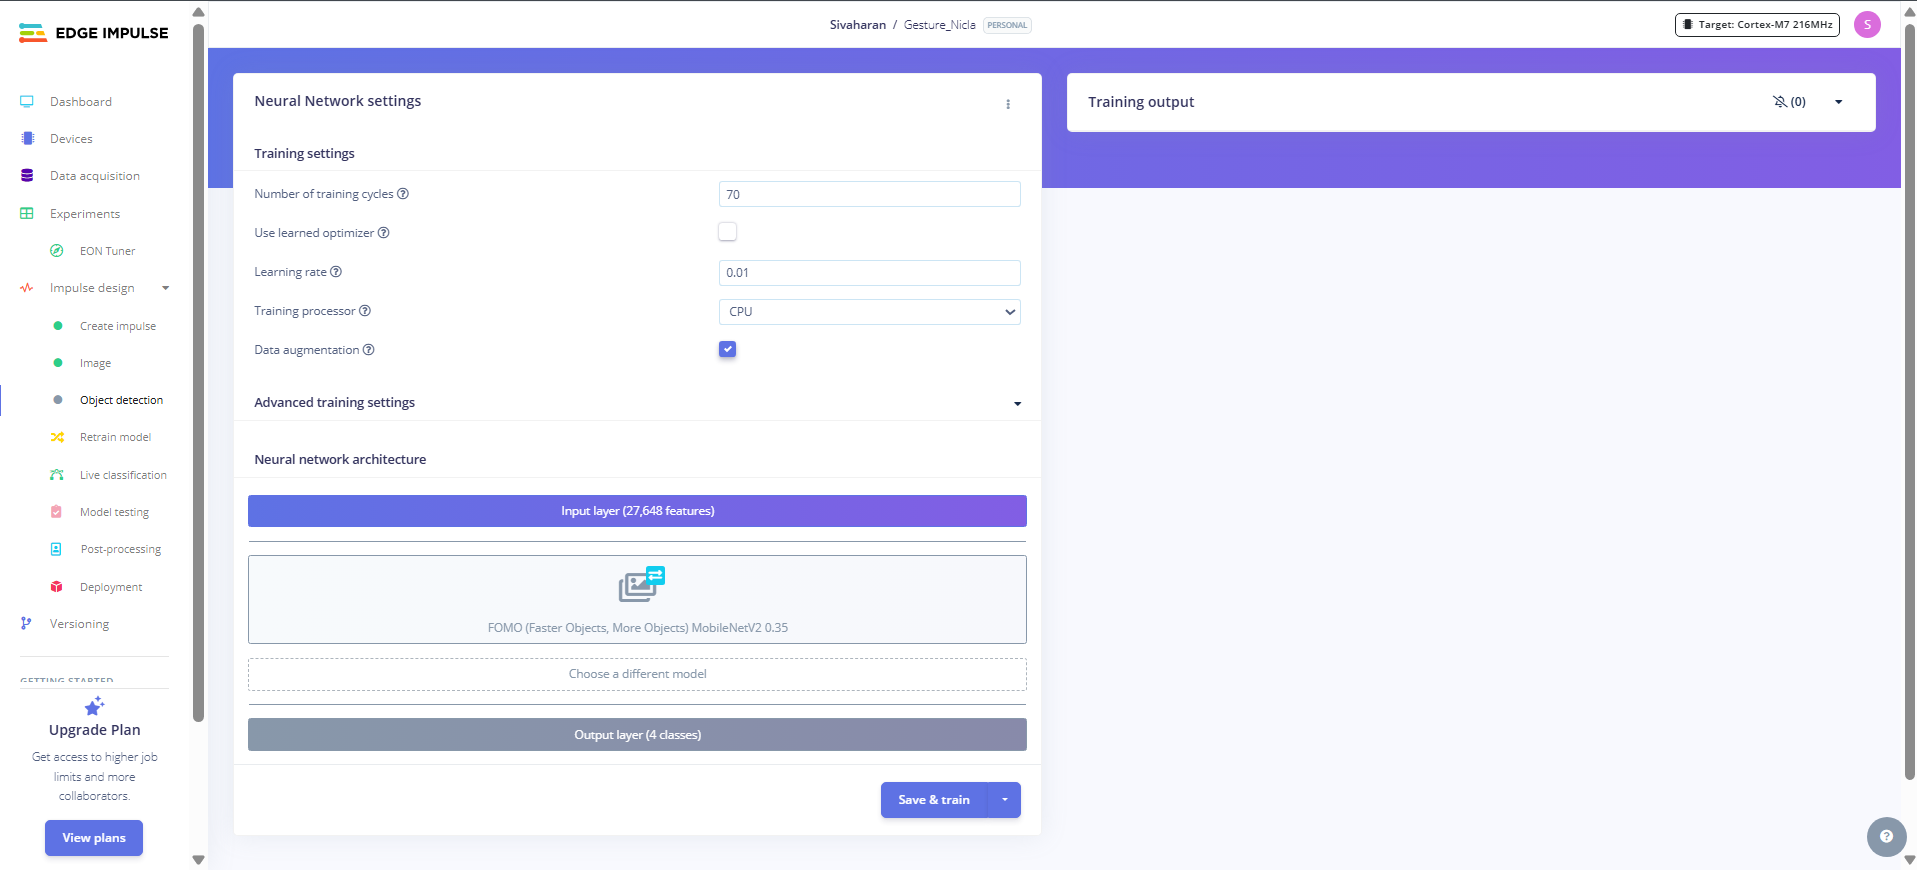
\includegraphics[width=\textwidth]{NiclaVision/Object_detected_parameters.png}
		\caption{Training parameters of the object-detection model (FOMO MobileNetV2 0.35)}
		\label{fig:nicla-train-params}
	\end{figure}
	
	The loss curve shows a rapid convergence in the first ten cycles, followed by a stabilisation, with no marked sign of overfitting between the training and validation curves.
	
	\begin{figure}[H]
		\centering
		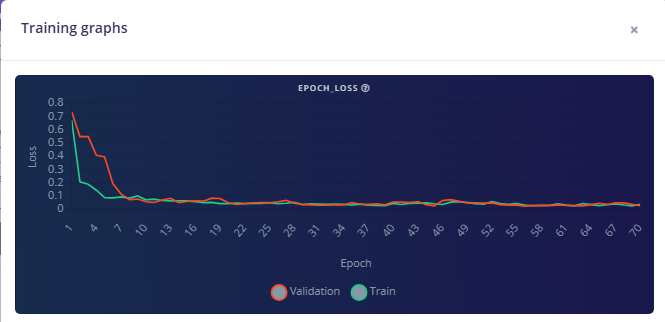
\includegraphics[width=0.75\textwidth]{NiclaVision/Loss_graph.png}
		\caption{Loss curve on the training and validation sets}
		\label{fig:nicla-loss}
	\end{figure}
	
	The final model reaches an F1 score of 92.3\% on the validation set. The confusion matrix shows perfect recognition of the Left, Right and Stop classes, and a lower score for Forward (F1 of 0.88), with 22.2\% of the Forward samples wrongly classified as background (non-detection), rather than confused with another gesture. The embedded-performance estimate for the complete model (DSP~+~neural network) amounts to 26~ms of inference time, 133.0~KB of peak RAM and 81.4~KB of flash.
	
	\begin{figure}[H]
		\centering
		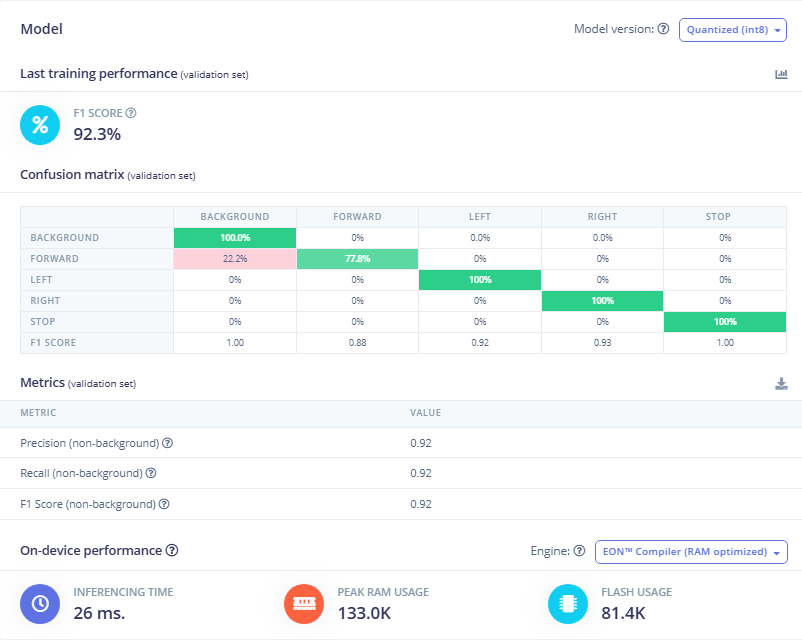
\includegraphics[width=0.75\textwidth]{NiclaVision/Trained_model.png}
		\caption{Results of the trained model (F1 92.3\%, confusion matrix, embedded performance)}
		\label{fig:nicla-trained-model}
	\end{figure}
	
	\subsection*{Deployment on the camera}
	
	The model was exported as a complete firmware specific to the Nicla Vision, in which the trained model is directly integrated, rather than loaded separately from a file. This firmware was flashed onto the board via the OpenMV IDE bootloader. Once flashed, the camera's folder contains, in addition to the firmware itself, a ready-to-use inference script as well as the raw model files, kept for reference.
	
	\begin{figure}[H]
		\centering
		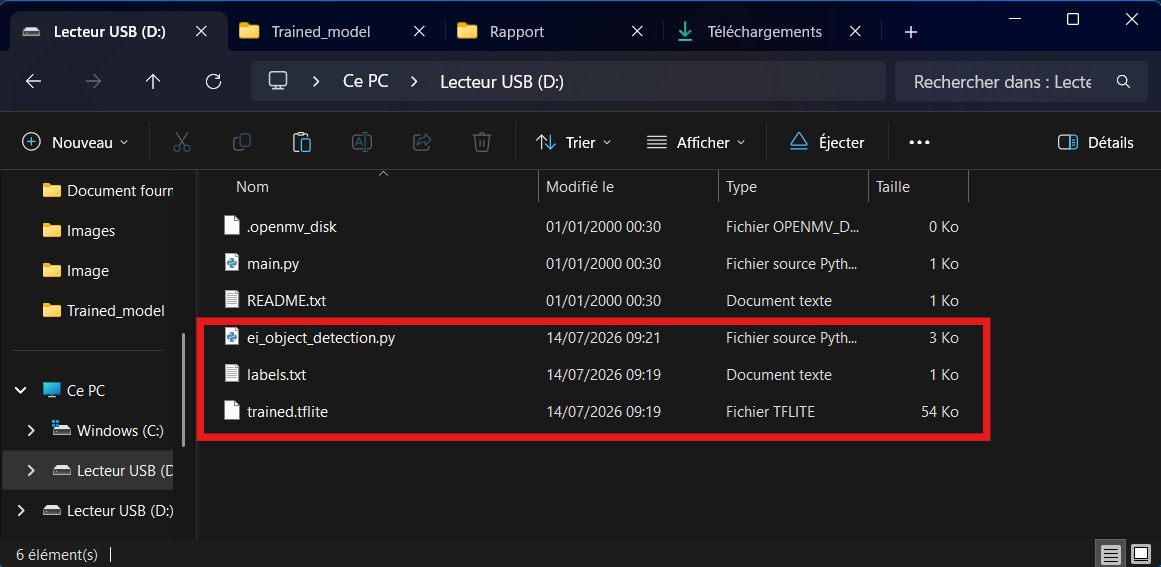
\includegraphics[width=0.6\textwidth]{NiclaVision/Fichier_dans_la_camera.png}
		\caption{Files present on the Nicla Vision disk after deployment}
		\label{fig:nicla-fichiers}
	\end{figure}
	
	The inference script (\texttt{main.py}) reuses the structure of the script provided by Edge Impulse, with two adaptations for the robot-control use case. \\ The line \texttt{model = ml.Model("trained")} directly loads the model integrated into the firmware, without going through a separate file. The \texttt{fomo\_post\_process()} function reuses the principle already presented in Section~4.2: extraction of the centroids per class from the output of the FOMO model, then filtering of the overlaps by NMS. The modification made concerns the main loop: rather than displaying the detail of each detection per class, the script keeps only the detection with the highest score in the image (\texttt{best\_label}, \texttt{best\_score}), and prints a single \texttt{DETECTED:<label>} line per image, a format directly usable by the control script on the PC side.
	
	\subsection*{Control script (\texttt{nicla\_to\_serial.py})}
	
	This script relays the detections from the Nicla Vision to the robot, reusing the mechanisms already put in place for the previous solutions (Section~3.2, Section~4.1). It continuously reads the camera's serial port, and applies an anti-false-positive temporal filter: a detection is only validated (\texttt{label\_valide}) after \texttt{CONFIRM\_COUNT} (5) identical consecutive detections, which limits the effect of an isolated erroneous detection. The validated label is then translated into a JSON command (\texttt{LABEL\_TO\_CMD}) and transmitted to the robot at a regular interval (\texttt{SEND\_INTERVAL}, 150~ms), with the same timeout safety mechanism (\texttt{TIMEOUT\_STOP}, 0.4~s) as for the other solutions. The \texttt{demarrer\_robot()} function performs the same software-restart sequence of the robot as for the WebCam and the HuskyLens.
	
	\subsection*{Software limitation encountered}
	
	During the control tests, an instability of the \texttt{ml.utils.NMS} function of the OpenMV firmware was observed: after working correctly for several tens of seconds to a few minutes, the execution of the model ends with an exception (\texttt{ml/utils.py}, in the constructor of the \texttt{NMS} class), returning the camera to the interactive prompt. This behaviour, already documented for this type of firmware, does not prevent occasional satisfactory operation, but introduces an instability that will need to be quantified precisely during the benchmark protocol.
	
	\subsection*{Results obtained}
	
	Despite this limitation, control of the robot by the Nicla Vision was successfully validated: the four gestures were correctly recognised and translated into commands, with the robot observed moving forward, stopping and turning in both directions in agreement with the gestures made in front of the camera.
	
	\begin{figure}[H]
		\centering
		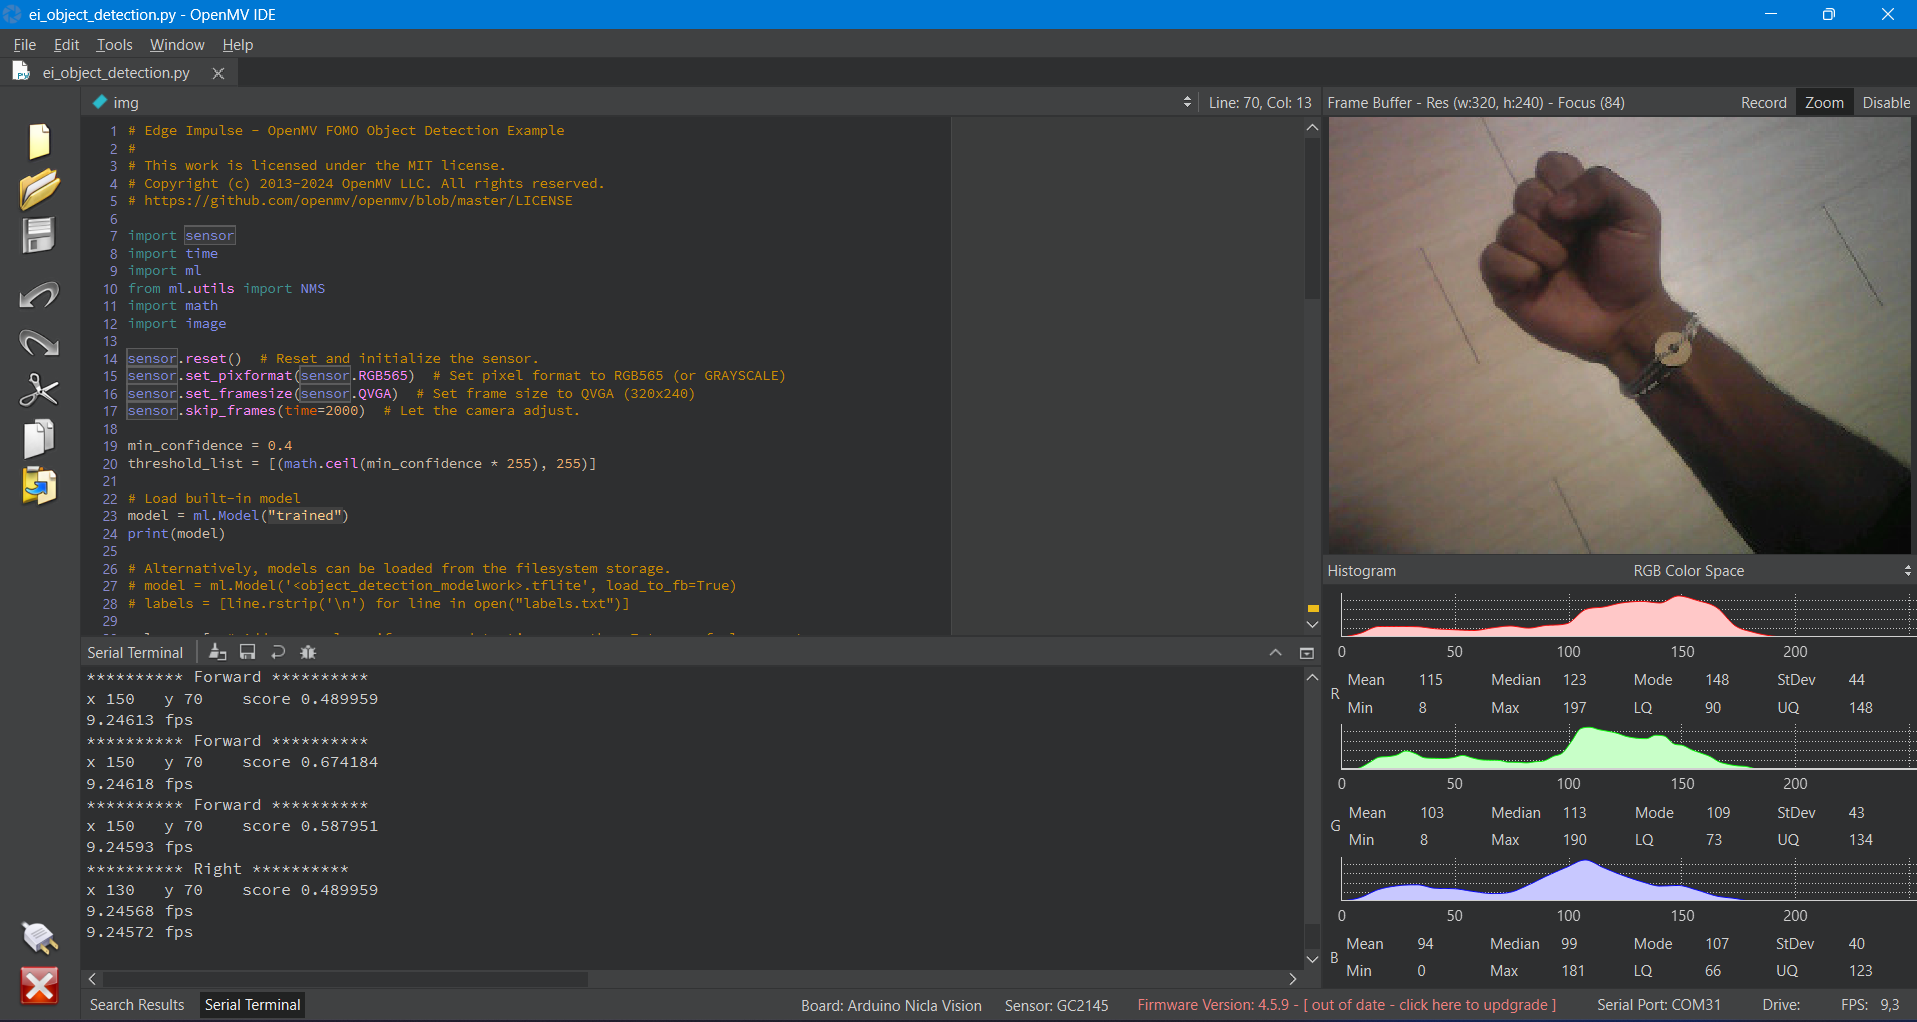
\includegraphics[width=\textwidth]{NiclaVision/Final_result.png}
		\caption{Live inference on the Nicla Vision in the OpenMV IDE (Forward and Right gestures detected)}
		\label{fig:nicla-final-result}
	\end{figure}
	
	The excerpt below, taken from the terminal of the \texttt{nicla\_to\_serial.py} script, illustrates the correct operation of the system, with the four commands exercised in succession:
	
	\begin{lstlisting}[language=bash, breaklines=true, basicstyle=\ttfamily\footnotesize]
		[Nicla] Left -> turn_left
		[Robot] b"x=0.000 y=0.000 angle=11.8 mode=turn_left dist=3.6"
		...
		[Nicla] Forward -> forward
		[Robot] b"x=0.000 y=0.000 angle=145.1 mode=forward dist=62.0"
		...
		[Nicla] Right -> turn_right
		[Robot] b"x=0.000 y=0.000 angle=-4.7 mode=turn_right dist=3.6"
		...
		[Nicla] Stop -> stop
		[Robot] b"x=0.000 y=0.000 angle=-104.1 mode=stop dist=22.4"
	\end{lstlisting}
	
	Recognition remains, however, less stable than for the WebCam or HuskyLens solutions: the \texttt{none} label (no valid detection) appears frequently even when a gesture is being held, reflecting a recognition reliability that could be improved, consistent with the lower F1 score obtained for the Forward class during training. This functional but imperfect behaviour is the basis on which the detailed benchmark protocol will be applied.
	
	\subsection*{Benchmark results}
	
	%=================================================================================
	%	NICLA VISION latency
	%=================================================================================
	
	\paragraph{Latency:} \mbox{} \\
	Latency was measured using a dedicated script (\texttt{benchmark\_latence\_nicla.py}), whose structure differs slightly from the one used for the WebCam. \textbf{Segment A (vision)} cannot be measured by a request/response round trip as for the HuskyLens in Section~4.4, since the Nicla Vision does not reply to a request but continuously pushes a \texttt{DETECTED:<label>} line per image processed, according to the protocol detailed above. \\ The \texttt{mesurer\_segment\_vision()} function therefore measures the time interval between two consecutive detection lines, which corresponds directly to the camera's own cycle time (capture, inference, centroid extraction, NMS filtering). \textbf{Segment B+C (communication)} reuses, without modification, the same ping/pong mechanism as for the WebCam and the HuskyLens, which we will see in the following subsection.
	
	A particularity of this script takes into account the software instability documented above: phase~1 is time-bounded (\texttt{SEGMENT\_A\_MAX\_DURATION}, 90~seconds), so that the script stops cleanly and exports the measurements already collected if the camera should crash before reaching the 100 targeted measurements, rather than remaining blocked indefinitely.
	
	\begin{table}[H]
		\centering
		\small
		\begin{tabular}{lccccc}
			\toprule
			\textbf{Latency} & \textbf{Mean} & \textbf{Median} & \textbf{Std. dev.} & \textbf{Min} & \textbf{Max} \\
			\midrule
			Segment A (vision) & 98.14~ms & 64.76~ms & 37.06~ms & 60.63~ms & 138.15~ms \\
			Segment B+C (comm.) & 5.86~ms & 4.02~ms & 4.37~ms & 3.11~ms & 19.20~ms \\
			\bottomrule
		\end{tabular}
		\caption{Latency of the Nicla Vision solution (95 and 88 measurements after warm-up)}
		\label{tab:latence-nicla}
	\end{table}
	
	\begin{figure}[H]
		\centering
		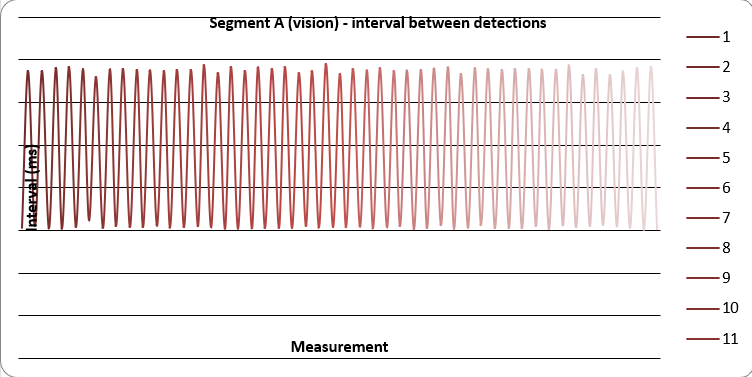
\includegraphics[width=0.8\textwidth]{NiclaVision/latence_vision_nicla.png}
		\caption{Latency per measurement for segment A (vision), interval between two successive detections}
		\label{fig:latence-vision-nicla}
	\end{figure}
	
	\begin{figure}[H]
		\centering
		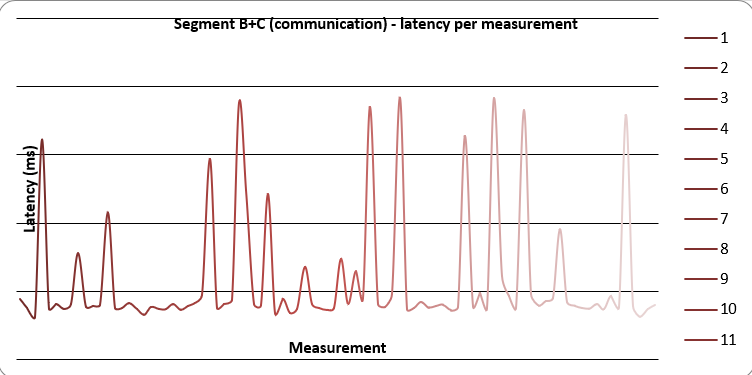
\includegraphics[width=0.8\textwidth]{NiclaVision/latence_comm_nicla.png}
		\caption{Latency per measurement for segment B+C (communication)}
		\label{fig:latence-comm-nicla}
	\end{figure}
	
	\paragraph{Analysis of the results:} \mbox{} \\
	The vision segment of the Nicla Vision (median 64.76~ms) is markedly slower than that of the WebCam (median 25.90~ms), which remains consistent with the chosen architecture, an object-detection model (FOMO) run entirely on a microcontroller, appreciably more costly in computation time than an internal classification model or PC-offloaded processing.
	
	Figure~\ref{fig:latence-vision-nicla} reveals a particular behaviour: the intervals alternate very regularly between two values, a short one (around 61~ms) and a long one (around 135~ms), forming a sawtooth pattern visible across the whole measurement, including during the warm-up phase. This stable alternation suggests a structural phenomenon rather than random measurement noise, for example related to the internal operation of the Nicla Vision's dual core or to the buffering of the messages sent over the serial port, without this hypothesis having been confirmed precisely. In this context, the median (64.76~ms) better reflects the most frequent interval than the mean (98.14~ms), pulled upwards by the alternation with the long intervals.
	
	The communication segment remains of the same order of magnitude as for the other solutions (median 4.02~ms versus 3.92~ms for the WebCam), which is expected since the code embedded on the robot is strictly identical. We note 7 pings out of 100 that went unanswered, a proportion comparable to that observed for the WebCam. The robot's startup log also shows an interrupt trace (\texttt{KeyboardInterrupt}) just before the software restart: this is the expected behaviour of the reset sequence, which deliberately interrupts a program already running on the robot before cleanly relaunching \texttt{code.py}, and not an error related to the benchmark.
	
	The total software latency stands at 103.99~ms on average and 68.78~ms in median, an order of magnitude that remains compatible with real-time control of the robot, although it approaches the human perceptibility threshold generally estimated between 100 and 150~ms, unlike the WebCam, which stays well clear of it.
	
	%=================================================================================
	%	NICLA VISION FPS
	%=================================================================================
	
	\paragraph{Throughput (FPS):} \mbox{} \\
	Throughput was measured using a dedicated script (\texttt{benchmark\_fps\_nicla.py}), built on the same principle as segment~A of the latency benchmark: the instantaneous throughput is computed as the inverse of the interval between two consecutive \texttt{DETECTED:<label>} lines ($\text{FPS} = 1/\Delta t$), rather than from an explicit capture loop as for the WebCam, since the Nicla Vision pushes its results continuously without being queried. The measurement lasts 30~seconds (\texttt{DUREE\_MESURE}), of which the first 3 seconds are excluded \\ (\texttt{WARMUP\_SEC}). Each interval is classified according to whether the gesture detected at that moment is active (\texttt{label != "none"}) or not, in order to distinguish the throughput in real use from the throughput at rest. As for the latency benchmark, the measurement remains time-bounded and stops cleanly with a warning if the serial link is interrupted along the way (already-documented \texttt{ml.utils.NMS} instability).
	
	\begin{table}[H]
		\centering
		\small
		\begin{tabular}{lccccc}
			\toprule
			\textbf{Throughput} & \textbf{Mean} & \textbf{Median} & \textbf{Std. dev.} & \textbf{Min} & \textbf{Max} \\
			\midrule
			Overall (275 images) & 11.82~FPS & 12.82~FPS & 4.45 & 7.09~FPS & 21.74~FPS \\
			Active gesture (231 images) & 11.84~FPS & 15.87~FPS & 4.45 & 7.09~FPS & 21.74~FPS \\
			No gesture (44 images) & 11.67~FPS & 8.00~FPS & 4.51 & 7.09~FPS & 21.28~FPS \\
			\bottomrule
		\end{tabular}
		\caption{Throughput (FPS) of the Nicla Vision solution (30~s measurement, warm-up excluded)}
		\label{tab:fps-nicla}
	\end{table}
	
	\begin{figure}[H]
		\centering
		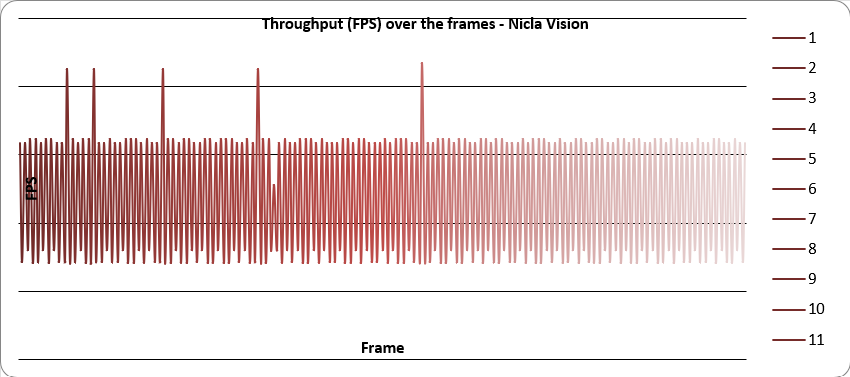
\includegraphics[width=0.9\textwidth]{NiclaVision/fps_nicla.png}
		\caption{Throughput (FPS) of the Nicla Vision solution over the images}
		\label{fig:fps-nicla}
	\end{figure}
	
	\paragraph{Analysis of the results:} \mbox{} \\
	The mean throughput of the Nicla Vision (11.82~FPS) is markedly lower than that of the WebCam (30.61~FPS), a gap consistent with the cycle times measured in the latency segment, the camera running the entire inference locally on a microcontroller rather than on a PC. The curve in Figure~5.28 shows the same sawtooth pattern as the one observed for latency: the throughput alternates regularly between two values, a high one (around 16~FPS, corresponding to the short interval of about 61~ms) and a low one (around 7~FPS, corresponding to the long interval of about 135~ms), which confirms that this is indeed a structural phenomenon of the camera's processing cycle, found consistently across both metrics.
	
	The curve also shows several occasional spikes, more spread out in time, exceeding 20~FPS. These spikes correspond to rare occurrences where two detections followed one another faster than the usual cycle, without a precise cause having been established.
	
	A counter-intuitive result is worth noting: the median throughput is higher when a gesture is active (15.87~FPS) than when no gesture is detected (8.00~FPS), the opposite of what one might expect if detecting an object increased the processing load. One possible explanation is that the short and long intervals are not evenly distributed between the two categories; the small numbers in the ``no gesture'' category (44 images versus 231) make this comparison fragile, and confirmation would require a measurement over a larger number of images.
	
	%=================================================================================
	%	NICLA VISION recognition reliability
	%=================================================================================
	
	\paragraph{Recognition reliability:} \mbox{} \\
	Reliability was measured using a dedicated script (\texttt{benchmark\_fiabilite\_nicla.py}), \\ which reuses the same manual protocol as the previous solutions: for each trial, the user makes a gesture in front of the camera then indicates, on the keyboard, the gesture they actually intended to make. Since the Nicla Vision has neither a screen nor a dedicated PC window, the keys are read in a non-blocking way (\texttt{msvcrt} library), in parallel with the continuous polling of the serial port. Unlike a simple reading of the raw detection, the script applies the same \textbf{temporal confirmation filter} as \texttt{nicla\_to\_serial.py} (5 identical consecutive detections required before validation, Section~4.3), so that the confusion matrix faithfully reflects the reliability as it is actually used to drive the robot, and not the image-by-image reliability. Each of the four gestures was repeated 20 times, i.e. 80 trials in total.
	
	\begin{table}[H]
		\centering
		\small
		\begin{tabular}{lccccc}
			\toprule
			\textbf{Intended \textbackslash\ Detected} & \textbf{Forward} & \textbf{Stop} & \textbf{Left} & \textbf{Right} & \textbf{Not detected} \\
			\midrule
			Forward & 13 & 0 & 0 & 0 & 7 \\
			Stop & 0 & 20 & 0 & 0 & 0 \\
			Left & 0 & 2 & 14 & 4 & 0 \\
			Right & 0 & 0 & 0 & 20 & 0 \\
			\bottomrule
		\end{tabular}
		\caption{Confusion matrix of the Nicla Vision solution (80 trials, 20 per gesture)}
		\label{tab:confusion-nicla}
	\end{table}
	
	\begin{figure}[H]
		\centering
		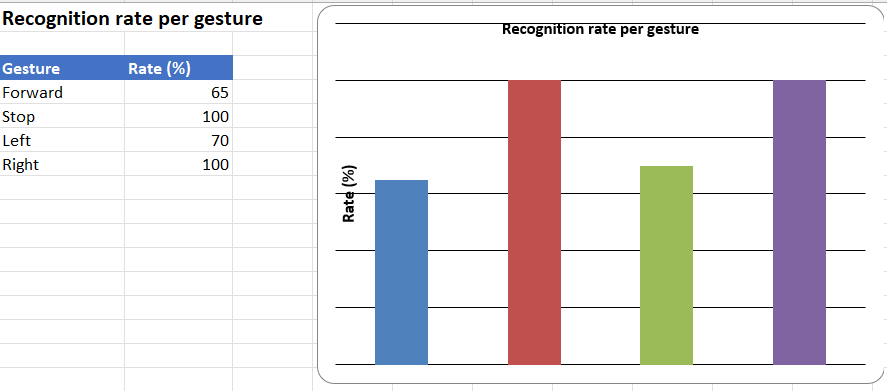
\includegraphics[width=0.7\textwidth]{NiclaVision/fiabilite_nicla.png}
		\caption{Recognition rate per gesture (Nicla Vision solution)}
		\label{fig:fiabilite-nicla}
	\end{figure}
	
	\paragraph{Analysis of the results:} \mbox{} \\
	The Nicla Vision solution achieves an overall recognition rate of 83.8\% (67/80), markedly lower than that of the WebCam (100\%), with results that are very contrasted depending on the gesture: Stop and Right are recognised perfectly (100\%), while Forward (65\%) and Left (70\%) concentrate almost all of the errors.
	
	Examining the detail of the trials reveals an interesting point: the errors are not distributed randomly within each series of 20, but clearly grouped. The 7 failures of the Forward gesture (classified as ``not detected'') correspond exactly to the first 7 trials of that series, the following 13 trials all being correctly recognised. Similarly, the 5 failures of the Left gesture (confused with Right or Stop) are concentrated almost entirely at the end of the series (trials 16 to 20 out of 20). This grouping suggests that the errors are less related to a structural confusion between gestures than to occasional factors specific to the test session, for example an adjustment time for the hand position at the start of the series for Forward, or fatigue and a progressive drift of the gesture performed at the end of the series for Left.
	
	This lower and more irregular reliability than that of the WebCam remains consistent with the observations made during training (Section~4.3). The F1 score of the Forward gesture (0.88) was already the lowest of the model, with a significant proportion of Forward samples wrongly classified as background, a flaw that is found directly in this benchmark result in the form of non-detections. It should be noted that there is a methodological limitation common to the reliability benchmarks of this project: the trials are carried out in a continuous series of 20 trials per gesture rather than in random order, which can favour the appearance of such grouping effects related to the user's learning or fatigue over the course of a single series, rather than to an intrinsic confusion of the model between the gestures themselves.
	
	\newpage
	
	%=================================================================================
	%	NICLA VISION consumption
	%=================================================================================
	
	\paragraph{Power consumption:} \mbox{} \\
	As for the WebCam, this last metric aimed to measure the electrical consumption of the camera using an INA219 module, placed in series on its power supply, in order to compare its consumption at rest and in active operation. This measurement would have been particularly relevant for the Nicla Vision: unlike the WebCam or the OpenMV M7, this board is explicitly designed for autonomous use on battery (Section~2.2.3), which makes its actual consumption directly related to its potential autonomy in an embedded application. A measurement would in particular have made it possible to quantify the energy cost of the dual core running continuously during inference, as well as that of peripherals unused in this project (Wi-Fi and Bluetooth connectivity, integrated on the board but not used by the robot control).
	
	This measurement could, as for the WebCam, not be carried out, for the same methodological reason: inserting an INA219 module on the camera's power supply requires temporarily cutting a power wire, a modification of the wiring that was not deemed advisable to make without explicit authorisation on hardware lent by the laboratory. This limitation, already set out in Section~4.1, therefore also applies to the Nicla Vision solution.
	
	\newpage
	
	%----------------------------------------------------------------------
	%	5.6 HuskyLens
	%----------------------------------------------------------------------
	
	\section{HuskyLens}
	
	\subsection*{Principle}
	
	Unlike the WebCam solution, where all of the vision processing is offloaded to the PC, the HuskyLens embeds its own processor and performs gesture recognition itself, through an internal \textit{Object Classification} algorithm presented in Section~2.2.4. It transmits to the PC only the already-computed result, a simple class identifier, and not an image to be processed.
	
	\subsection*{Architecture adopted}
	
	The camera remains fixed in a stationary position facing the user, like the webcam, so that it does not lose sight of the user during the robot's turns. An architecture with an intermediate microcontroller dedicated to reading the HuskyLens had initially been considered, before being abandoned. The HuskyLens in fact natively has a micro-USB port allowing direct serial communication with the PC, making this intermediary unnecessary. The architecture adopted therefore connects the HuskyLens to the PC over USB, the PC acting as a simple lightweight relay to the robot over a second USB port, without performing any image analysis itself, the processing intelligence remaining entirely embedded in the camera.
	
	\subsection*{Installation and identification of the serial port}
	
	Communication with the HuskyLens from the PC relies on the official Python library \texttt{HUSKYLENSPython}~\cite{huskylenspython_repo}, distributed as a single file (\texttt{huskylib.py}) rather than via \texttt{pip}, to be downloaded manually from its GitHub repository and placed in the project folder. Two additional dependencies are installed via \texttt{pip}: \texttt{pyserial} and \texttt{pypng}.
	
	The HuskyLens used embeds a CP2102N (Silicon Labs) USB-to-serial interface chip, different from the more common CH340 chip found on this type of module. The corresponding driver (\textit{CP210x USB to UART Bridge VCP Drivers})~\cite{cp210x_driver} must be installed for the serial port to be recognised by Windows. Once the driver is installed, the assigned COM port can be identified directly from PowerShell:
	
	\begin{lstlisting}[language=bash]
		Get-PnpDevice -PresentOnly -Class Ports | Select-Object FriendlyName, InstanceId
	\end{lstlisting}
	
	The port sought appears under a name of the type \textit{Silicon Labs CP210x USB to UART Bridge (COMx)}.
	
	\subsection*{Communication library (\texttt{huskylib.py})}
	
	This official library implements the proprietary protocol of the HuskyLens, based on binary frames with a fixed header and a checksum. It exposes a \texttt{HuskyLensLibrary} class, instantiated in serial mode (\texttt{"SERIAL"}), which sends a connection-check frame (\texttt{knock()}) at startup, selects the active algorithm \\ (\texttt{algorthim("ALGORITHM\_OBJECT\_CLASSIFICATION")}), and provides methods for learning (\texttt{learn()}) and for reading the already-learned objects (\texttt{learned()}). The detected objects are represented by the \texttt{Block} (bounding rectangle, with a class identifier) or \texttt{Arrow} classes, depending on the algorithm used.
	
	\subsection*{Training the gestures (\texttt{huskylens\_training.py})}
	
	The HuskyLens is used in \textit{Object Classification} mode, which makes it possible to learn several object classes and assign them a numeric identifier. Five classes were defined, summarised in Table~\ref{tab:husky-mapping}, a fifth ``Neutral'' class serving as a reference when no hand is present in front of the camera.
	
	\begin{table}[H]
		\centering
		\begin{tabular}{cl}
			\toprule
			\textbf{ID} & \textbf{Gesture} \\
			\midrule
			1 & Forward (closed fist) \\
			2 & Stop (open hand) \\
			3 & Left (index + thumb) \\
			4 & Right (index + pinky) \\
			5 & Neutral (no hand / rest position) \\
			\bottomrule
		\end{tabular}
		\caption{Mapping of the HuskyLens identifiers to the gestures}
		\label{tab:husky-mapping}
	\end{table}
	
	Rather than using the camera's physical buttons, training was automated by the \\ \texttt{huskylens\_training.py} script. For each gesture, the \\ \texttt{rafale\_apprentissage()} function splits the acquisition into two batches of 50 captures (\texttt{N\_LOTS}, \texttt{N\_PAR\_LOT}), at a rate of one capture per second, with a pause between the two batches (validated by a key press) allowing the user to reposition themselves. Each call to \texttt{hl.learn(gesture\_id)} adds a new sample to the corresponding class without overwriting the previous ones, for a total of 100 samples per gesture, well above the minimum of 30 photos per class recommended by the manufacturer for good recognition accuracy~\cite{dfrobot_huskylens}.
	
	\subsection*{Control script (\texttt{huskylens\_to\_serial.py})}
	
	This script reuses the same JSON protocol as the WebCam solution (Section~4.1), \\ the HuskyLens having already determined the gesture, the script simply translates the received identifier into a command and transmits it to the robot. The \texttt{lire\_id\_geste()} function queries the camera via \texttt{hl.learned()} and returns the identifier of the recognised class, or \texttt{None} if nothing is detected. A temporal confirmation filter (\texttt{CONFIRM\_COUNT}, 5 identical consecutive detections) limits the effect of occasional false positives, exactly on the same principle as the one already used for the Nicla Vision (Section~4.3). The validated identifier is then translated into a command (\texttt{ID\_TO\_COMMAND}) and transmitted to the robot at a regular interval (\texttt{SEND\_INTERVAL}, 150~ms), with the same software-restart sequence of the robot as for the previous solutions.
	
	Thanks to the complete reuse of the JSON protocol established in Section~3.2, no modification of the code embedded on the robot was necessary: \texttt{code.py}, \texttt{robot.py}, \\ \texttt{pid\_controller.py} and \texttt{pio\_encoder.py} remain strictly identical to those used for the WebCam solution.
	
	\subsection*{Difficulties encountered and solutions applied}
	
	\begin{itemize}
		\item \textbf{USB-serial chip not recognised.} The HuskyLens port did not appear in any list of serial ports, including in PowerShell. The initial hypothesis of a CH340 chip (the most common on this type of module) turned out to be wrong, the camera actually embedding a CP2102N chip from Silicon Labs, requiring a specific driver. Solution: installing the official CP210x driver.
		\item \textbf{Behaviour of \texttt{learned()} not conforming to the documentation.} The method is documented as returning a list of detected objects, but actually returns a single object directly when a gesture is detected. This behaviour, not conforming to the official documentation, is a known bug documented in the project's repository~\cite{huskylenspython_issue18} (see the comment of the \texttt{lire\_id\_geste()} function in the code). Solution: directly handling the returned object via \texttt{getattr(objet, "ID", None)}, without list indexing.
		\item \textbf{Robot not reacting despite commands being correctly sent.} During the first tests, the script did display the detected gestures and the corresponding commands, but the robot did not move. The cause was identical to the one already encountered for the WebCam (Section~4.1): the absence of a software restart of the robot, which could remain stuck at the interactive prompt without running \texttt{code.py}. Solution: adding the same restart sequence as for the WebCam, before any command is sent.
	\end{itemize}
	
	\newpage
	
	\subsection*{Benchmark results}
	
	%=================================================================================
	%	HUSKYLENS latency
	%=================================================================================
	
	\paragraph{Latency:} \mbox{} \\
	Latency was measured using a dedicated script (\texttt{benchmark\_latence\_huskylens.py}), in two distinct segments. Unlike the WebCam solution where the PC performs the inference itself, the HuskyLens has already determined the gesture internally, so \textbf{segment A} does not measure vision processing, but the camera's response time to a simple serial request (\texttt{hl.learned()}), timed on the PC side over 100 iterations. \textbf{Segment B+C (communication)} reuses, without any modification, the same ping/pong mechanism already used for the WebCam and the Nicla Vision, which is possible since the code embedded on the robot (\texttt{code.py}) remained strictly identical from one solution to another. The first 15 measurements of segment~A and the first 5 of segment~B+C are excluded from the statistics (warm-up).
	
	\begin{table}[H]
		\centering
		\small
		\begin{tabular}{lccccc}
			\toprule
			\textbf{Latency} & \textbf{Mean} & \textbf{Median} & \textbf{Std. dev.} & \textbf{Min} & \textbf{Max} \\
			\midrule
			Segment A (HuskyLens) & 2.94~ms & 2.01~ms & 3.36~ms & 1.63~ms & 23.07~ms \\
			Segment B+C (comm.) & 5.06~ms & 3.84~ms & 3.05~ms & 3.20~ms & 17.30~ms \\
			\bottomrule
		\end{tabular}
		\caption{Latency of the HuskyLens solution (85 and 86 measurements after warm-up)}
		\label{tab:latence-husky}
	\end{table}
	
	\begin{figure}[H]
		\centering
		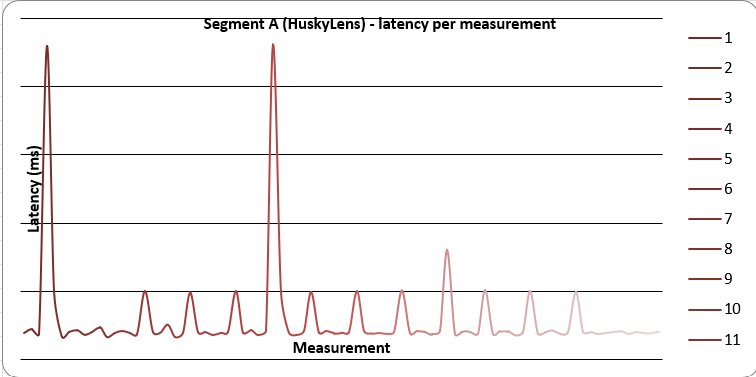
\includegraphics[width=0.8\textwidth]{HuskyLens/latence_husky_A.png}
		\caption{Latency per measurement for segment A (HuskyLens request)}
		\label{fig:latence-husky-a}
	\end{figure}
	
	\begin{figure}[H]
		\centering
		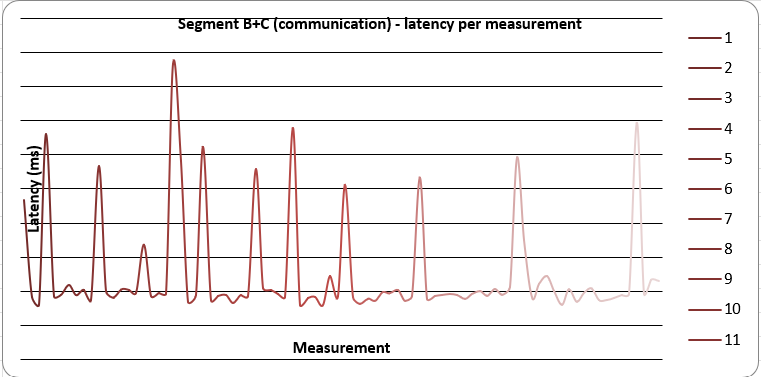
\includegraphics[width=0.8\textwidth]{HuskyLens/latence_husky_comm.png}
		\caption{Latency per measurement for segment B+C (communication)}
		\label{fig:latence-husky-comm}
	\end{figure}
	
	\paragraph{Analysis of the results:} \mbox{} \\
	The HuskyLens request segment (median 2.01~ms) is markedly faster than the vision segment of the WebCam solution (median 25.90~ms) and than the detection segment of the Nicla Vision (median 64.76~ms). This result is consistent with the architecture of this camera: the PC here only waits for a serial response to a request already processed continuously by the HuskyLens's internal processor, without having to trigger an inference itself.
	
	The communication segment remains of the same order of magnitude as for the other solutions (median 3.84~ms), which is expected since the robot code is identical. We note 9 pings out of 100 that went unanswered, a loss that, as for the WebCam, worsens progressively over the course of the session (0 losses after 10 sends, 5 after 60, 9 after 100), which confirms that this is probably a phenomenon specific to the robot rather than to the camera used.
	
	The total software latency stands at 8.00~ms on average and 5.85~ms in median, the lowest measured so far among the tested solutions. This raw result should nevertheless be qualified: the anti-false-positive filtering (5 identical consecutive detections required before validating a gesture change, Section~4.4) in practice adds a further confirmation delay not counted here, before a gesture change is actually transmitted to the robot.
	
	\newpage
	
	%=================================================================================
	%	HUSKYLENS FPS
	%=================================================================================
	
	\paragraph{Throughput (FPS):} \mbox{} \\
	Throughput was measured using a dedicated script (\texttt{benchmark\_fps\_huskylens.py}), built on the same principle as segment~A of the latency benchmark: the \texttt{mesurer\_fps()} function queries the HuskyLens in a continuous loop via \texttt{hl.learned()} for 30~seconds \\ (\texttt{DUREE\_MESURE}), the instantaneous throughput being computed as the inverse of the duration of each request ($\text{FPS} = 1/\Delta t$). The first 3 seconds are excluded from the statistics (\texttt{WARMUP\_SEC}). Each request is classified according to whether the returned identifier corresponds to an active gesture (ID 1 to 4) or to the neutral class / absence of detection (\texttt{ID\_NEUTRE}, ID~5), in order to distinguish the throughput in real use from the throughput at rest, on the same principle as for the WebCam and the Nicla Vision.
	
	\begin{table}[H]
		\centering
		\footnotesize\setlength{\tabcolsep}{4pt}
		\begin{tabular}{lccccc}
			\toprule
			\textbf{Throughput} & \textbf{Mean} & \textbf{Median} & \textbf{Std. dev.} & \textbf{Min} & \textbf{Max} \\
			\midrule
			Overall (9,187 requests) & 445.10~FPS & 492.08~FPS & 132.42 & 31.06~FPS & 853.97~FPS \\
			Active gesture (8,304 requests) & 445.16~FPS & 491.97~FPS & 132.50 & 31.06~FPS & 853.97~FPS \\
			Neutral (883 requests) & 444.50~FPS & 493.02~FPS & 131.68 & 34.82~FPS & 745.49~FPS \\
			\bottomrule
		\end{tabular}
		\caption{Throughput (FPS) of the HuskyLens solution (30~s measurement, warm-up excluded)}
		\label{tab:fps-husky}
	\end{table}
	
	\begin{figure}[H]
		\centering
		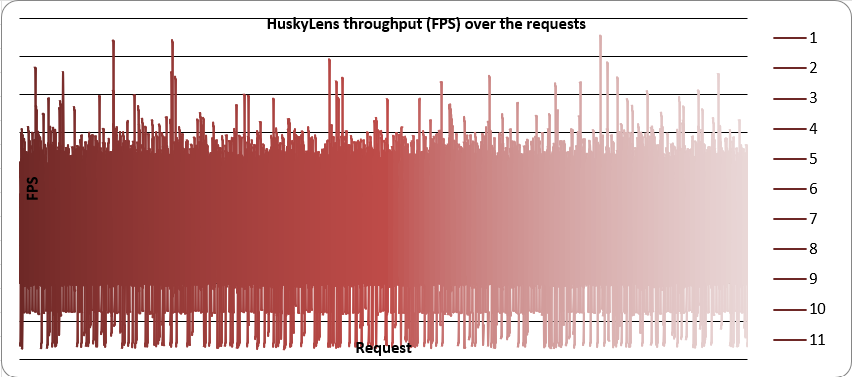
\includegraphics[width=0.9\textwidth]{HuskyLens/fps_husky.png}
		\caption{Throughput (FPS) of the HuskyLens solution over the requests}
		\label{fig:fps-husky}
	\end{figure}
	
	\paragraph{Analysis of the results:} \mbox{} \\
	The query throughput of the HuskyLens (median 492.08~FPS) is very largely higher than that of all the other solutions measured so far (WebCam: 31.62~FPS, Nicla Vision: 12.82~FPS), the serial request being much lighter than complete image processing. This figure must, however, be interpreted with caution: it corresponds to the speed at which the PC can query the HuskyLens's serial port, and not to an actual refresh rate of the camera's internal recognition, which could renew its result at a lower frequency without this being visible from this measurement.
	
	The standard deviation is high (132.42, i.e. about 30\% of the mean), reflecting a markedly greater instability than for the other solutions. The curve in Figure~\ref{fig:fps-husky} confirms this observation: rather than a continuous variation, it shows recurring latency plateaus (visible around 500, 200 and 40~FPS in the raw data), probably due to fixed internal timings of the camera's USB-serial controller rather than to a variable processing load.
	
	As for the WebCam and the Nicla Vision, the presence of an active gesture does not appreciably affect the throughput (445.16~FPS versus 444.50~FPS for the neutral position), a result consistent with the fact that recognition takes place continuously in the camera, independently of the speed at which the PC reads the result.
	
	%=================================================================================
	%	HUSKYLENS recognition reliability
	%=================================================================================
	
	\paragraph{Recognition reliability:} \mbox{} \\
	Reliability was measured using a dedicated script (\texttt{benchmark\_fiabilite\_huskylens.py}), adapted from the script used for the WebCam. Since the HuskyLens does not have a PC window (it has its own integrated screen), the keys are read in the console in a non-blocking way (\texttt{msvcrt}), while the camera is continuously queried via \texttt{lire\_id\_geste()}. The protocol remains identical to the previous solutions: for each trial, the user makes a gesture in front of the camera (while watching its integrated screen) then indicates, on the keyboard, the gesture they actually intended to make. The script displays live the gesture currently detected as well as the progress of each of the four counters, which makes it possible to follow the progress without leaving the console. Each of the four gestures was repeated 20 times, i.e. 80 trials in total.
	
	\begin{table}[H]
		\centering
		\small
		\begin{tabular}{lccccc}
			\toprule
			\textbf{Intended \textbackslash\ Detected} & \textbf{Forward} & \textbf{Stop} & \textbf{Left} & \textbf{Right} & \textbf{Not detected} \\
			\midrule
			Forward & 15 & 5 & 0 & 0 & 0 \\
			Stop & 0 & 20 & 0 & 0 & 0 \\
			Left & 0 & 2 & 18 & 0 & 0 \\
			Right & 0 & 3 & 1 & 16 & 0 \\
			\bottomrule
		\end{tabular}
		\caption{Confusion matrix of the HuskyLens solution (80 trials, 20 per gesture)}
		\label{tab:confusion-husky}
	\end{table}
	
	\begin{figure}[H]
		\centering
		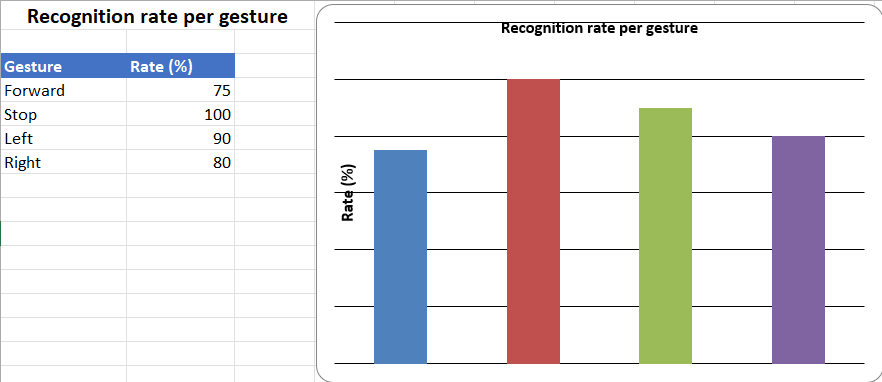
\includegraphics[width=0.7\textwidth]{HuskyLens/fiabilite_husky.png}
		\caption{Recognition rate per gesture (HuskyLens solution)}
		\label{fig:fiabilite-husky}
	\end{figure}
	
	\paragraph{Analysis of the results:} \mbox{} \\
	The HuskyLens solution achieves an overall recognition rate of 86.2\% (69/80), an intermediate result between the WebCam (100\%) and the Nicla Vision (83.8\%). Only the Stop gesture is recognised perfectly (100\%); the three other gestures each show a proportion of errors, all classified as Stop or confused with one another, without any trial remaining completely ``not detected''.
	
	The confusion matrix reveals a notable imbalance: the Stop class concentrates almost all of the errors of the three other gestures (5 errors for Forward, 2 for Left, 3 for Right), suggesting that it acts as a ``default'' class towards which the model falls back in case of uncertainty, rather than a symmetric confusion between visually close gestures. The Right gesture furthermore shows an occasional confusion with Left (1 trial out of 20), consistent with the visual proximity already identified for the Left (index~+~thumb) and Right (index~+~pinky) gestures during the design of the gestures in Section~4.1.
	
	This rate of 86.2\%, although lower than that of the WebCam, remains very largely sufficient for functional gesture control of the robot, and constitutes an additional differentiating point of comparison between the studied architectures, a camera whose recognition relies on an embedded classification model more constrained than a complete library such as MediaPipe.
	
	%=================================================================================
	%	HUSKYLENS consumption
	%=================================================================================
	
	\paragraph{Power consumption:} \mbox{} \\
	As for the previous solutions, this last metric aimed to measure the electrical consumption of the HuskyLens using an INA219 module, placed in series on its power supply, in order to compare its consumption at rest and in active operation. This measurement would have been particularly interesting for this camera: its very high query throughput (previous section) suggests a USB-serial controller solicited continuously, whose actual energy cost remains, at this stage, purely speculative.
	
	This measurement could, as for the previous solutions, not be carried out, for the same methodological reason: inserting an INA219 module on the camera's power supply requires temporarily cutting a power wire, a modification of the wiring that was not deemed advisable to make without explicit authorisation on hardware lent by the laboratory. This limitation, already set out in Section~4.1, therefore also applies to the HuskyLens solution.
	
	%----------------------------------------------------------------------
	%	5.7 OAK-D Lite
	%----------------------------------------------------------------------
	
	\section{OAK-D Lite}
	
	The OAK-D Lite is the fifth and last vision solution studied in this benchmark, added on the recommendation of my supervisor (Section~1.1) in order to broaden the comparison to a camera embedding a dedicated vision processor markedly more powerful than the four previous architectures.
	
	\subsection*{Principle and architecture}
	
	The OAK-D Lite is built around the Intel Movidius Myriad~X vision processor, presented in the technical overview in Section~2.2.5. Development relies on the open-source DepthAI ecosystem from Luxonis~\cite{depthai_docs}, which makes it possible to define a processing pipeline (capture, resizing, inference) run directly on the Myriad~X chip. As for the HuskyLens and the Nicla Vision, the host PC only acts as a lightweight relay to the robot, without performing any vision processing itself.
	
	A first minimal script (\texttt{test\_connexion.py}), a simple camera pipeline followed by an OpenCV display, made it possible to validate detection of the device and the USB link before any acquisition step.
	
	\subsection*{Building the dataset (\texttt{capture\_dataset.py})}
	
	The \texttt{capture\_dataset.py} script captures an image at each key press (\texttt{1}~=~forward, \texttt{2}~=~stop, \texttt{3}~=~left, \texttt{4}~=~right), automatically saved into the subfolder corresponding to its gesture. In total, 160 images were captured, at a rate of 40 per gesture, following the same protocol as for the Nicla Vision (Section~4.3).
	
	\begin{figure}[H]
		\centering
		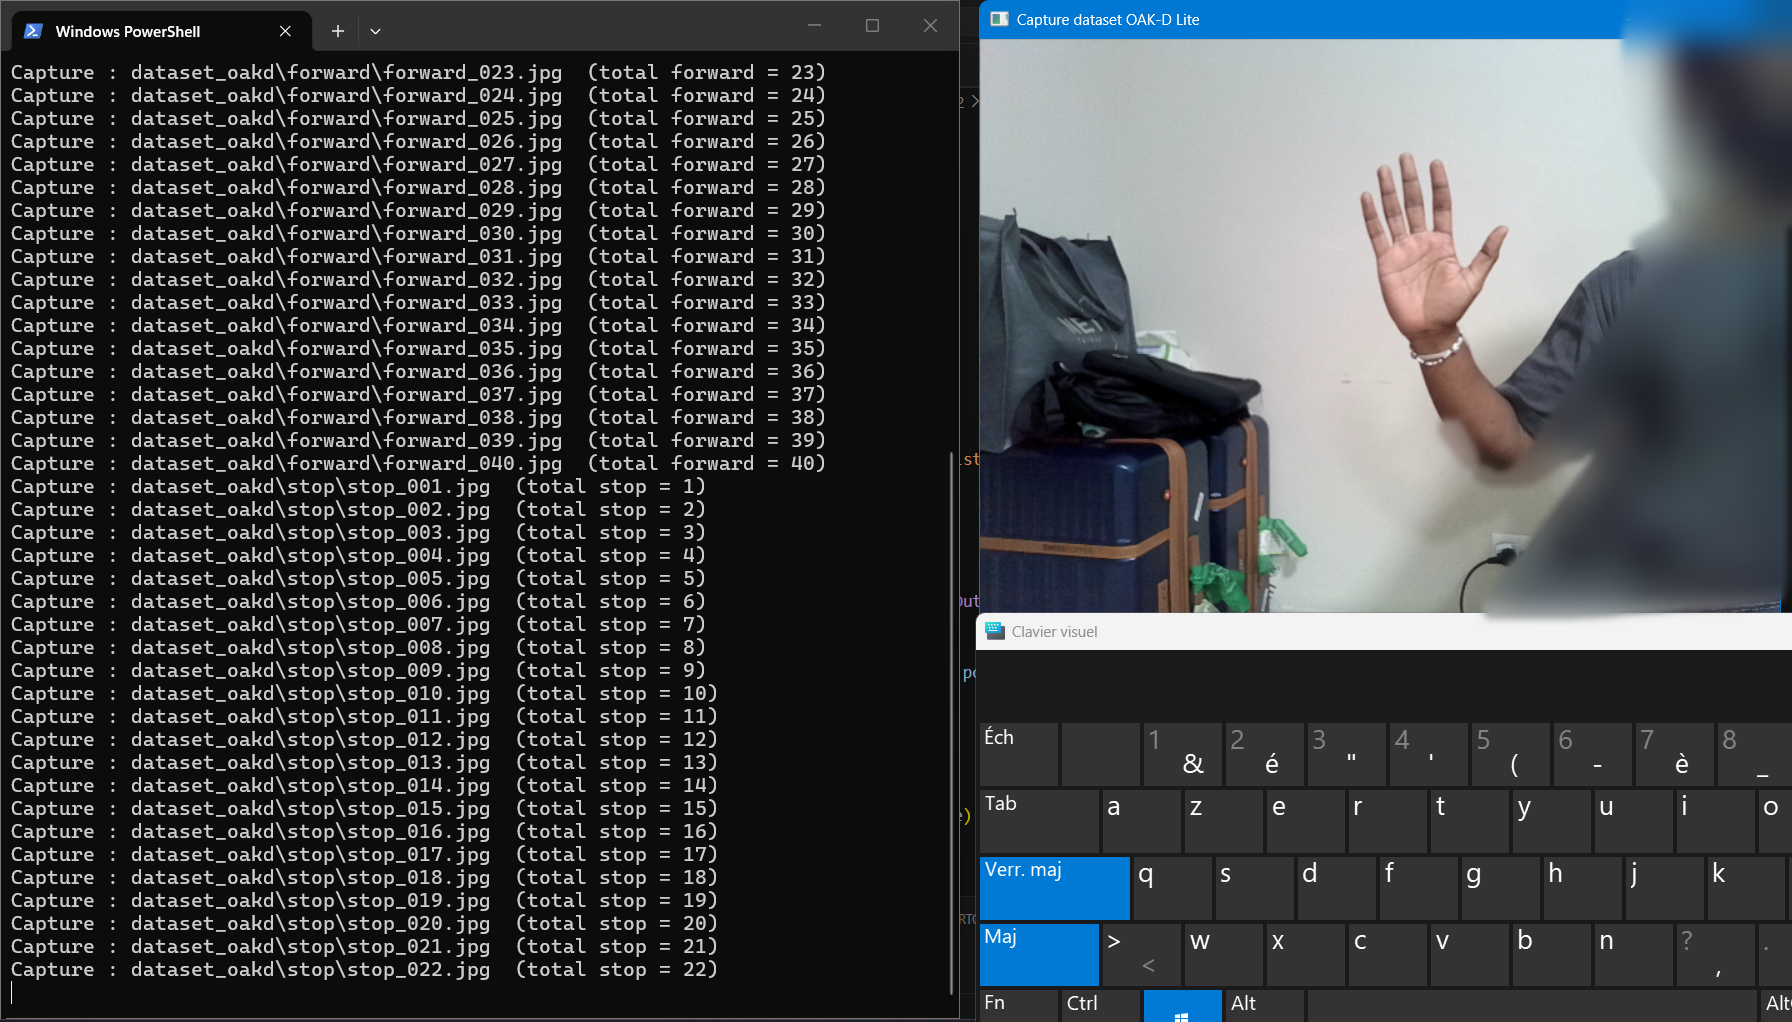
\includegraphics[width=0.85\textwidth]{OAKD/oakd_capture_gestes.png}
		\caption{Dataset capture with the OAK-D Lite}
		\label{fig:oakd-capture}
	\end{figure}
	
	\subsection*{Labelling and dataset preparation}
	
	Unlike the webcam and the cameras with internal classification, object detection requires precisely locating the gesture within the image, and not merely classifying it. The labelling of the 160 images (drawing a bounding box around the hand, with its associated gesture) was carried out in Edge Impulse Studio, split into 127 training images and 33 test images.
	
	\begin{figure}[H]
		\centering
		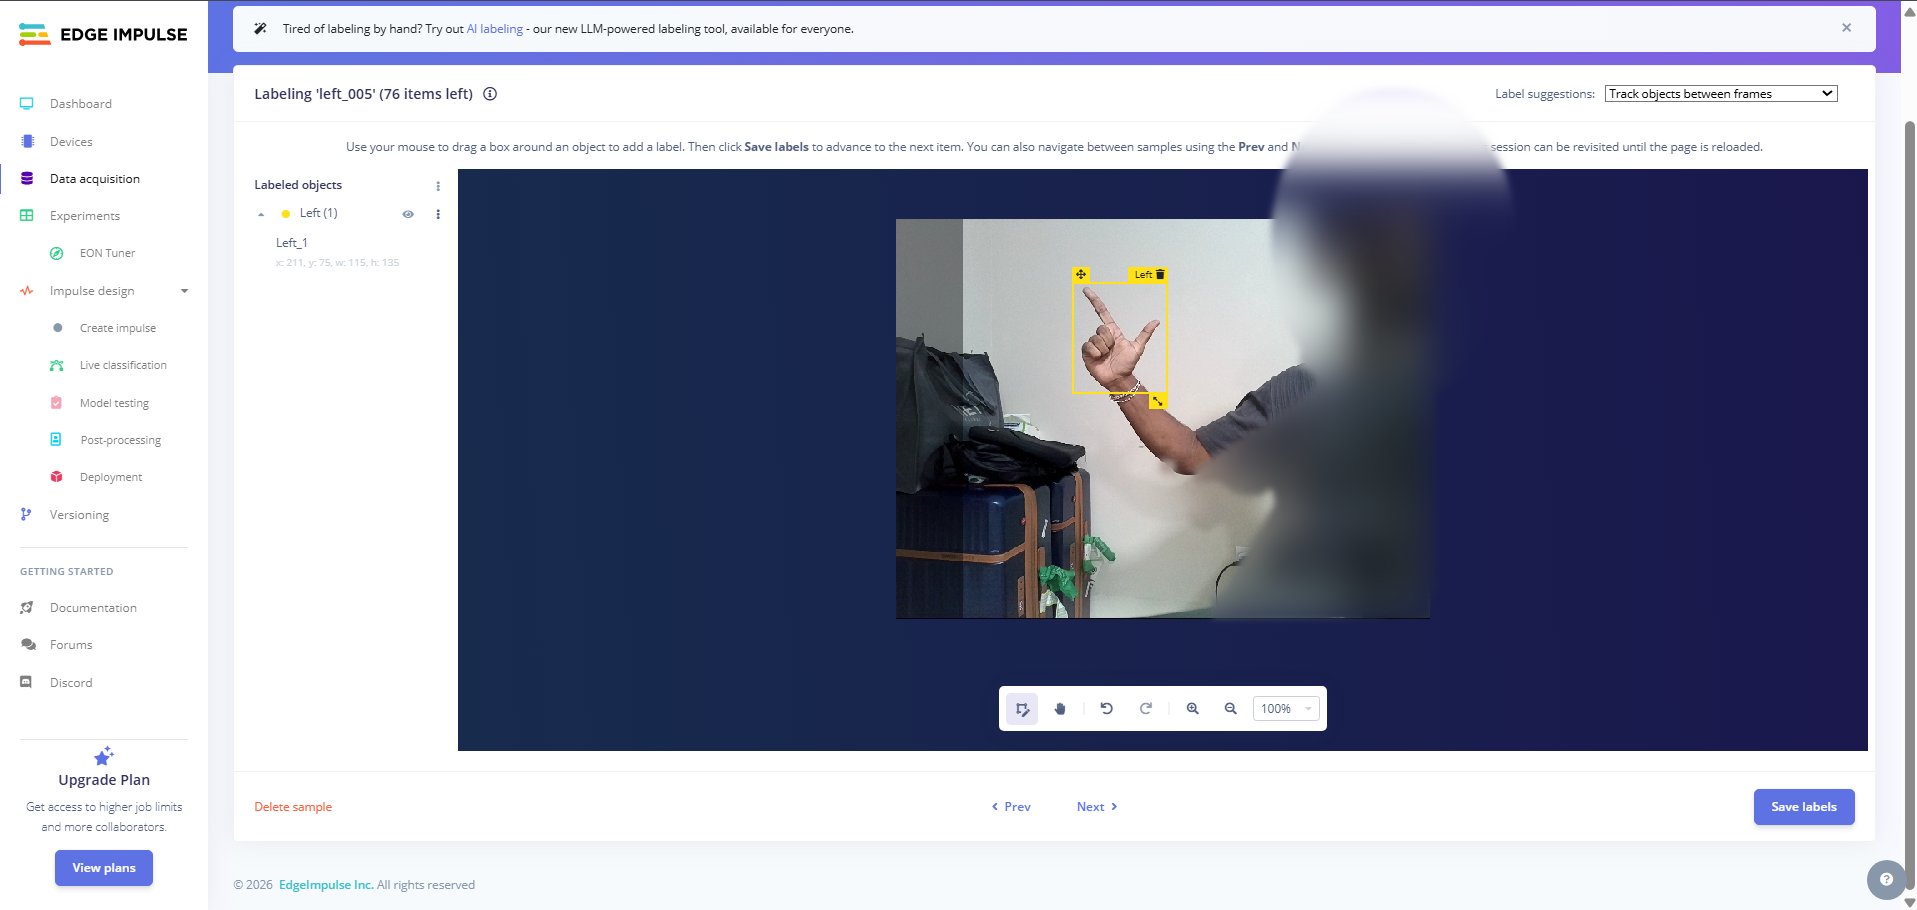
\includegraphics[width=0.85\textwidth]{OAKD/oakd_etiquetage_ei.png}
		\caption{Manual labelling of the images by bounding box in Edge Impulse}
		\label{fig:oakd-etiquetage}
	\end{figure}
	
	\begin{figure}[H]
		\centering
		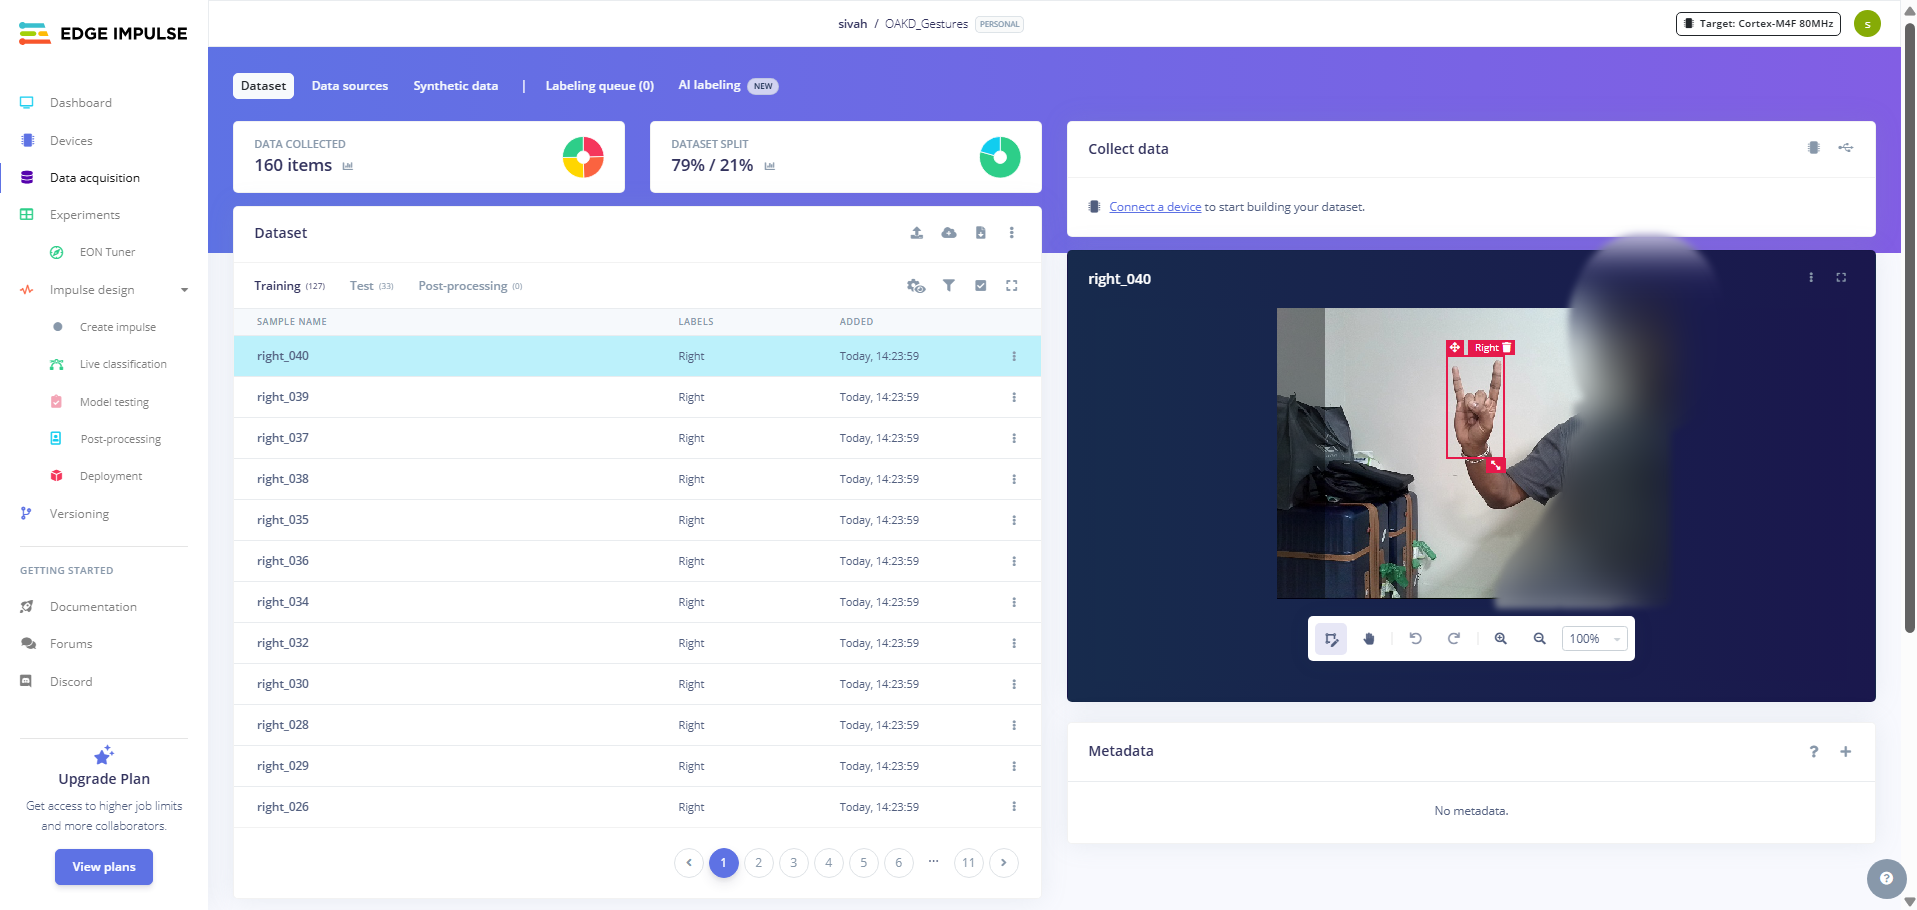
\includegraphics[width=0.85\textwidth]{OAKD/oakd_images_etiquetees.png}
		\caption{Labelled dataset in Edge Impulse (160 images, 4 classes)}
		\label{fig:oakd-images-etiquetees}
	\end{figure}
	
	Since the model was trained outside Edge Impulse with Ultralytics YOLOv8n (for reasons of compatibility with the Myriad~X conversion chain, detailed later), the dataset was exported from Edge Impulse in the native \texttt{info.labels} format (a JSON file listing, for each image, its training/test category and its bounding boxes), then converted by the \texttt{prepare\_yolo\_dataset.py} script to the structure expected by Ultralytics. For each image, the bounding boxes in pixels are converted to the normalised YOLO format (centre coordinates and dimensions relative to the image size, between 0 and 1), the images and annotation files being distributed across the \texttt{images/train}, \texttt{images/val}, \texttt{labels/train} and \texttt{labels/val} folders. The script also generates the \texttt{gestures.yaml} configuration file, which associates each numeric class identifier with its name (0~=~Forward, 1~=~Left, 2~=~Right, 3~=~Stop).
	
	\subsection*{Training (\texttt{entrainer.py})}
	
	The model was trained with the Ultralytics library~\cite{ultralytics_yolov8}, from the pre-trained model \texttt{yolov8n.pt} (the lightest of the YOLOv8 family, suited to embedded deployment), over 100 epochs, with an image size of 320$\times$320 and a batch size of 8.
	
	\begin{figure}[H]
		\centering
		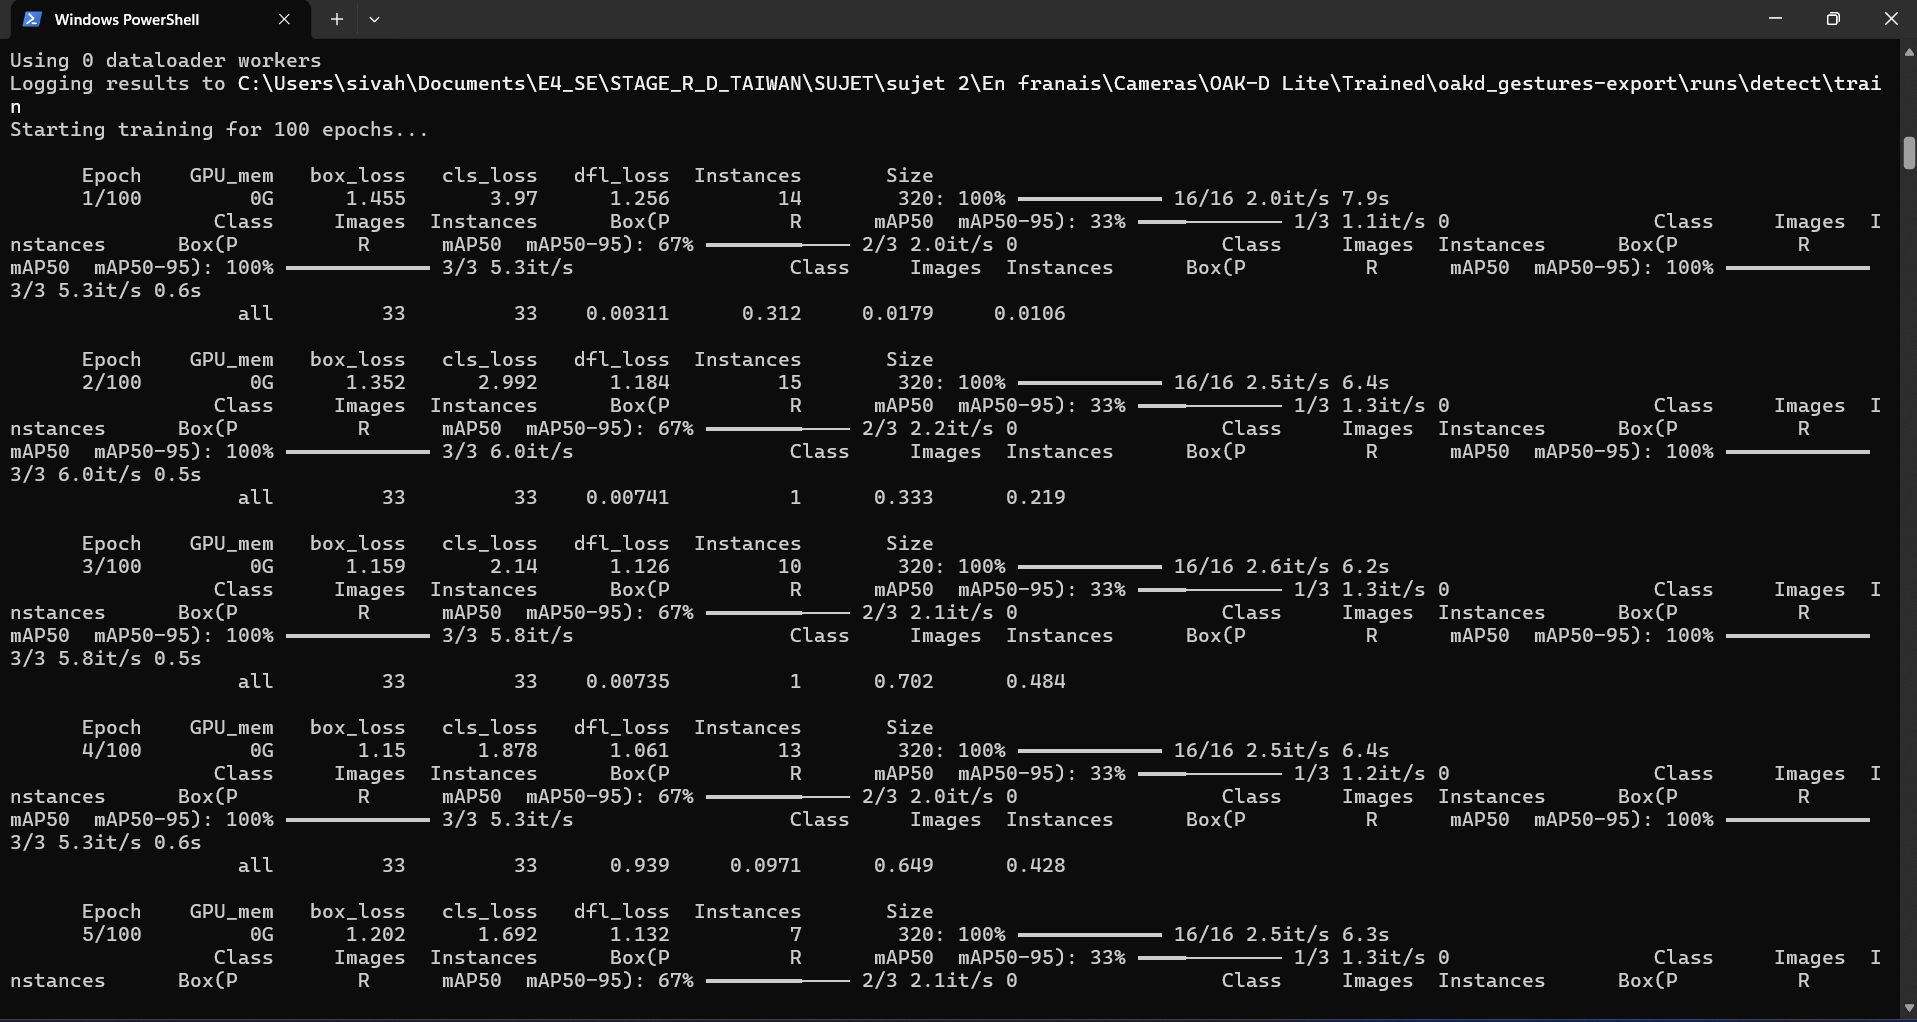
\includegraphics[width=0.95\textwidth]{OAKD/oakd_entrainement.png}
		\caption{Console log during the first training epochs}
		\label{fig:oakd-console}
	\end{figure}
	
	At the end of the training, the model reaches an accuracy of 95.7\%, a recall of 96.9\%, a mAP50 of 96.6\% and a mAP50-95 of 72.3\% on the validation set. Figure~\ref{fig:oakd-courbes} shows a rapid convergence of all the metrics within the first twenty epochs, followed by a stabilisation, except for a persistent variability on the validation losses (\texttt{val/box\_loss}, \texttt{val/dfl\_loss}), consistent with the limited size of the validation set.
	
	\begin{figure}[H]
		\centering
		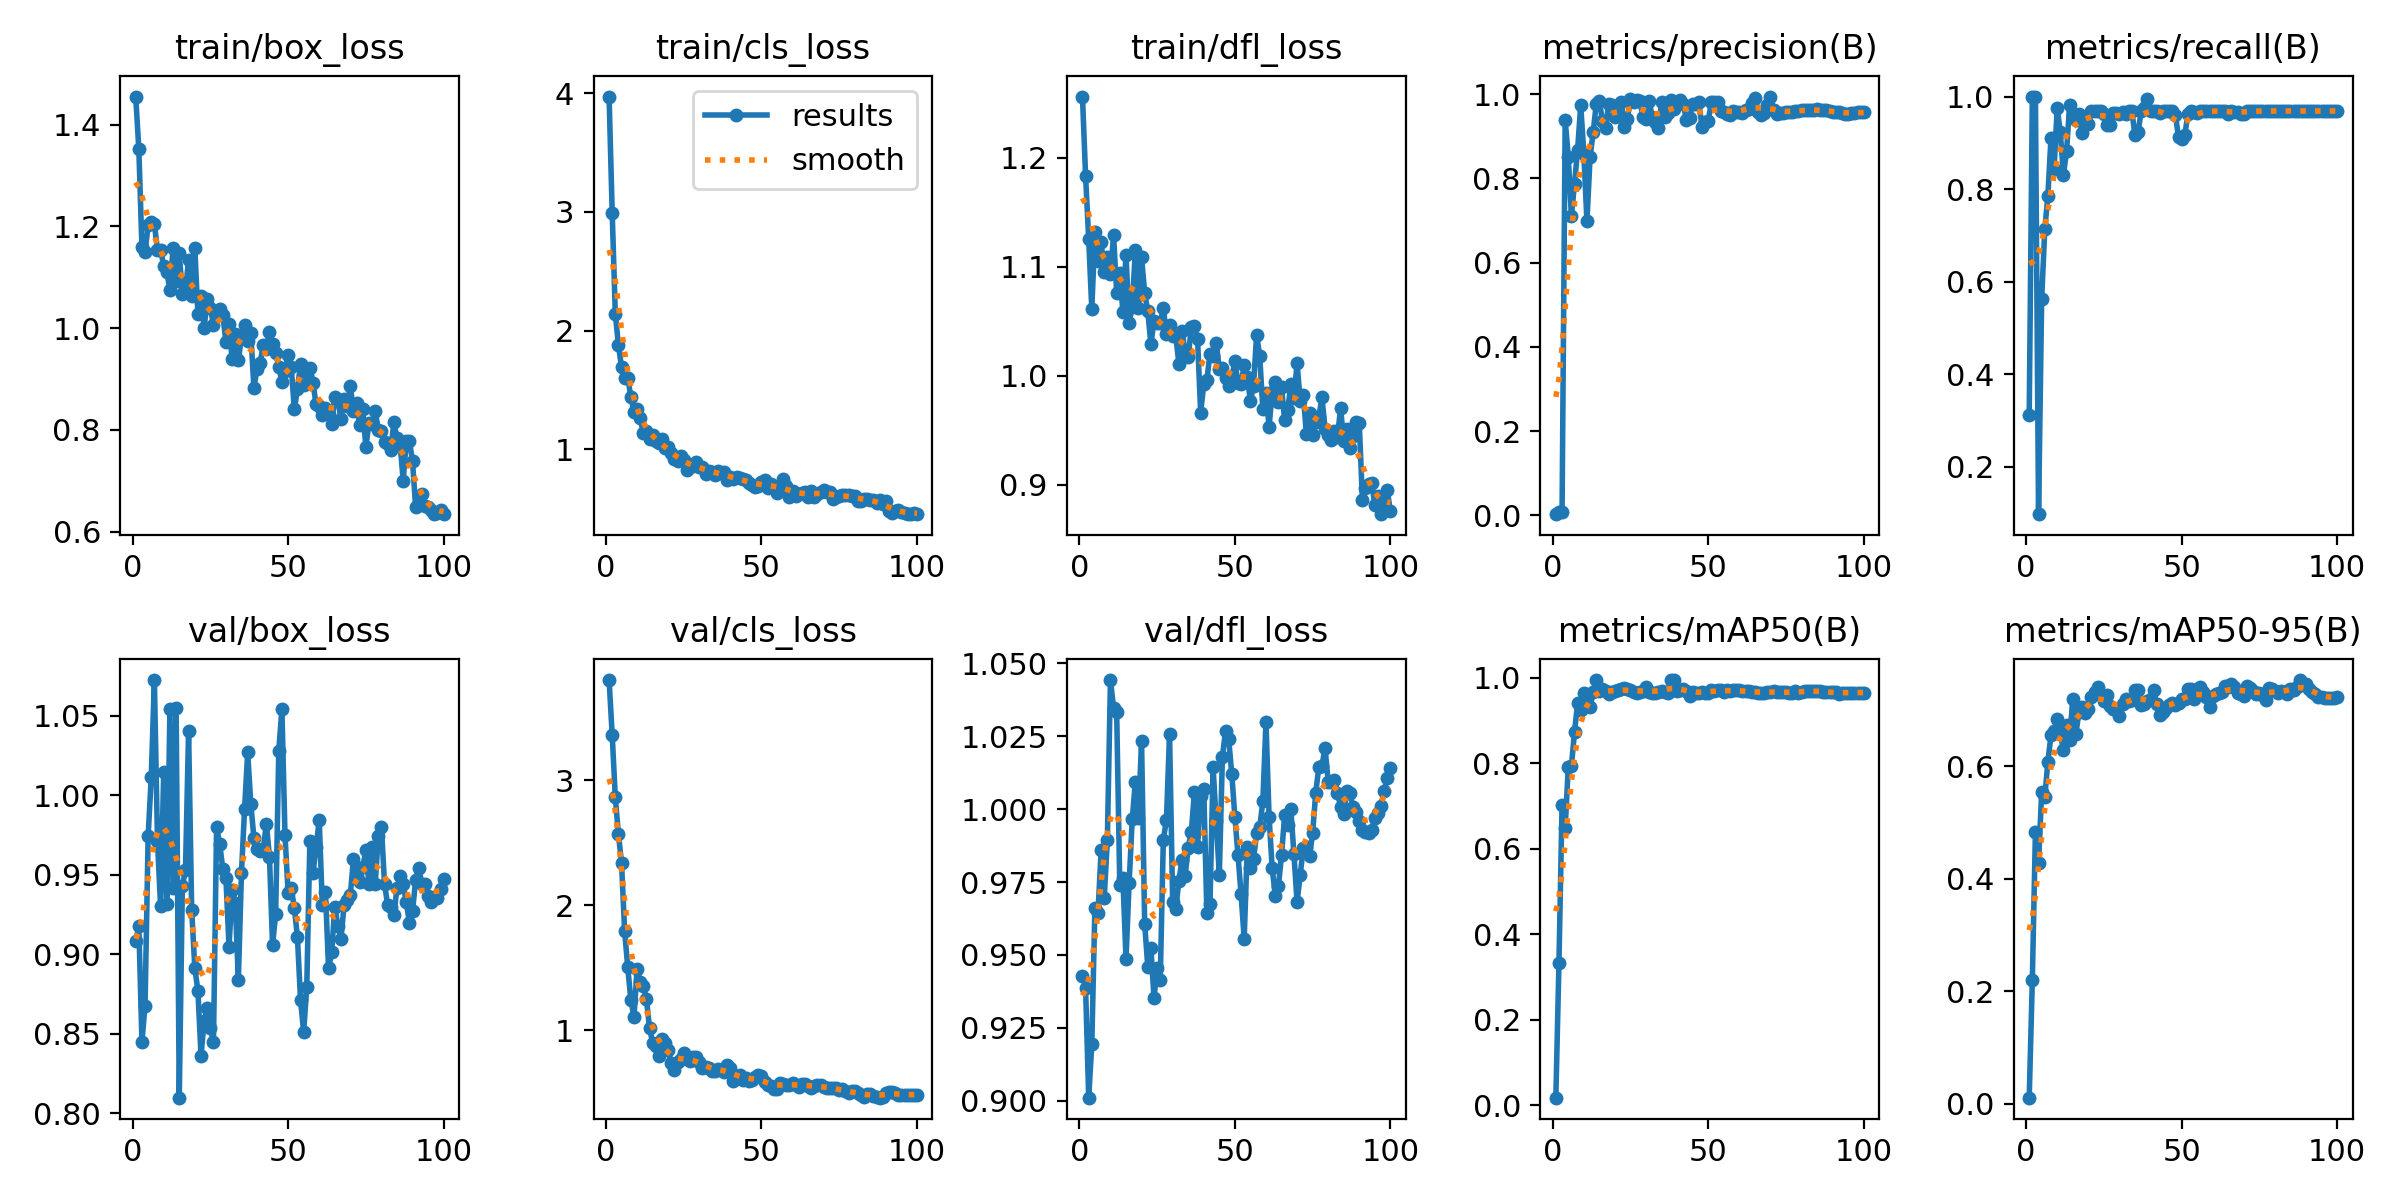
\includegraphics[width=\textwidth]{OAKD/oakd_courbes_entrainement.png}
		\caption{Evolution of the losses and metrics (accuracy, recall, mAP) over the 100 training epochs}
		\label{fig:oakd-courbes}
	\end{figure}
	
	The normalised confusion matrix (Figure~\ref{fig:oakd-matrice-entrainement}) details the performance per gesture: Forward, Left and Stop are classified with perfect accuracy (100\%), while the Right gesture reaches 87\%, the remaining 13\% not being confused with another gesture but classified as background (non-detection), rather than a confusion between visually close gestures.
	
	\begin{figure}[H]
		\centering
		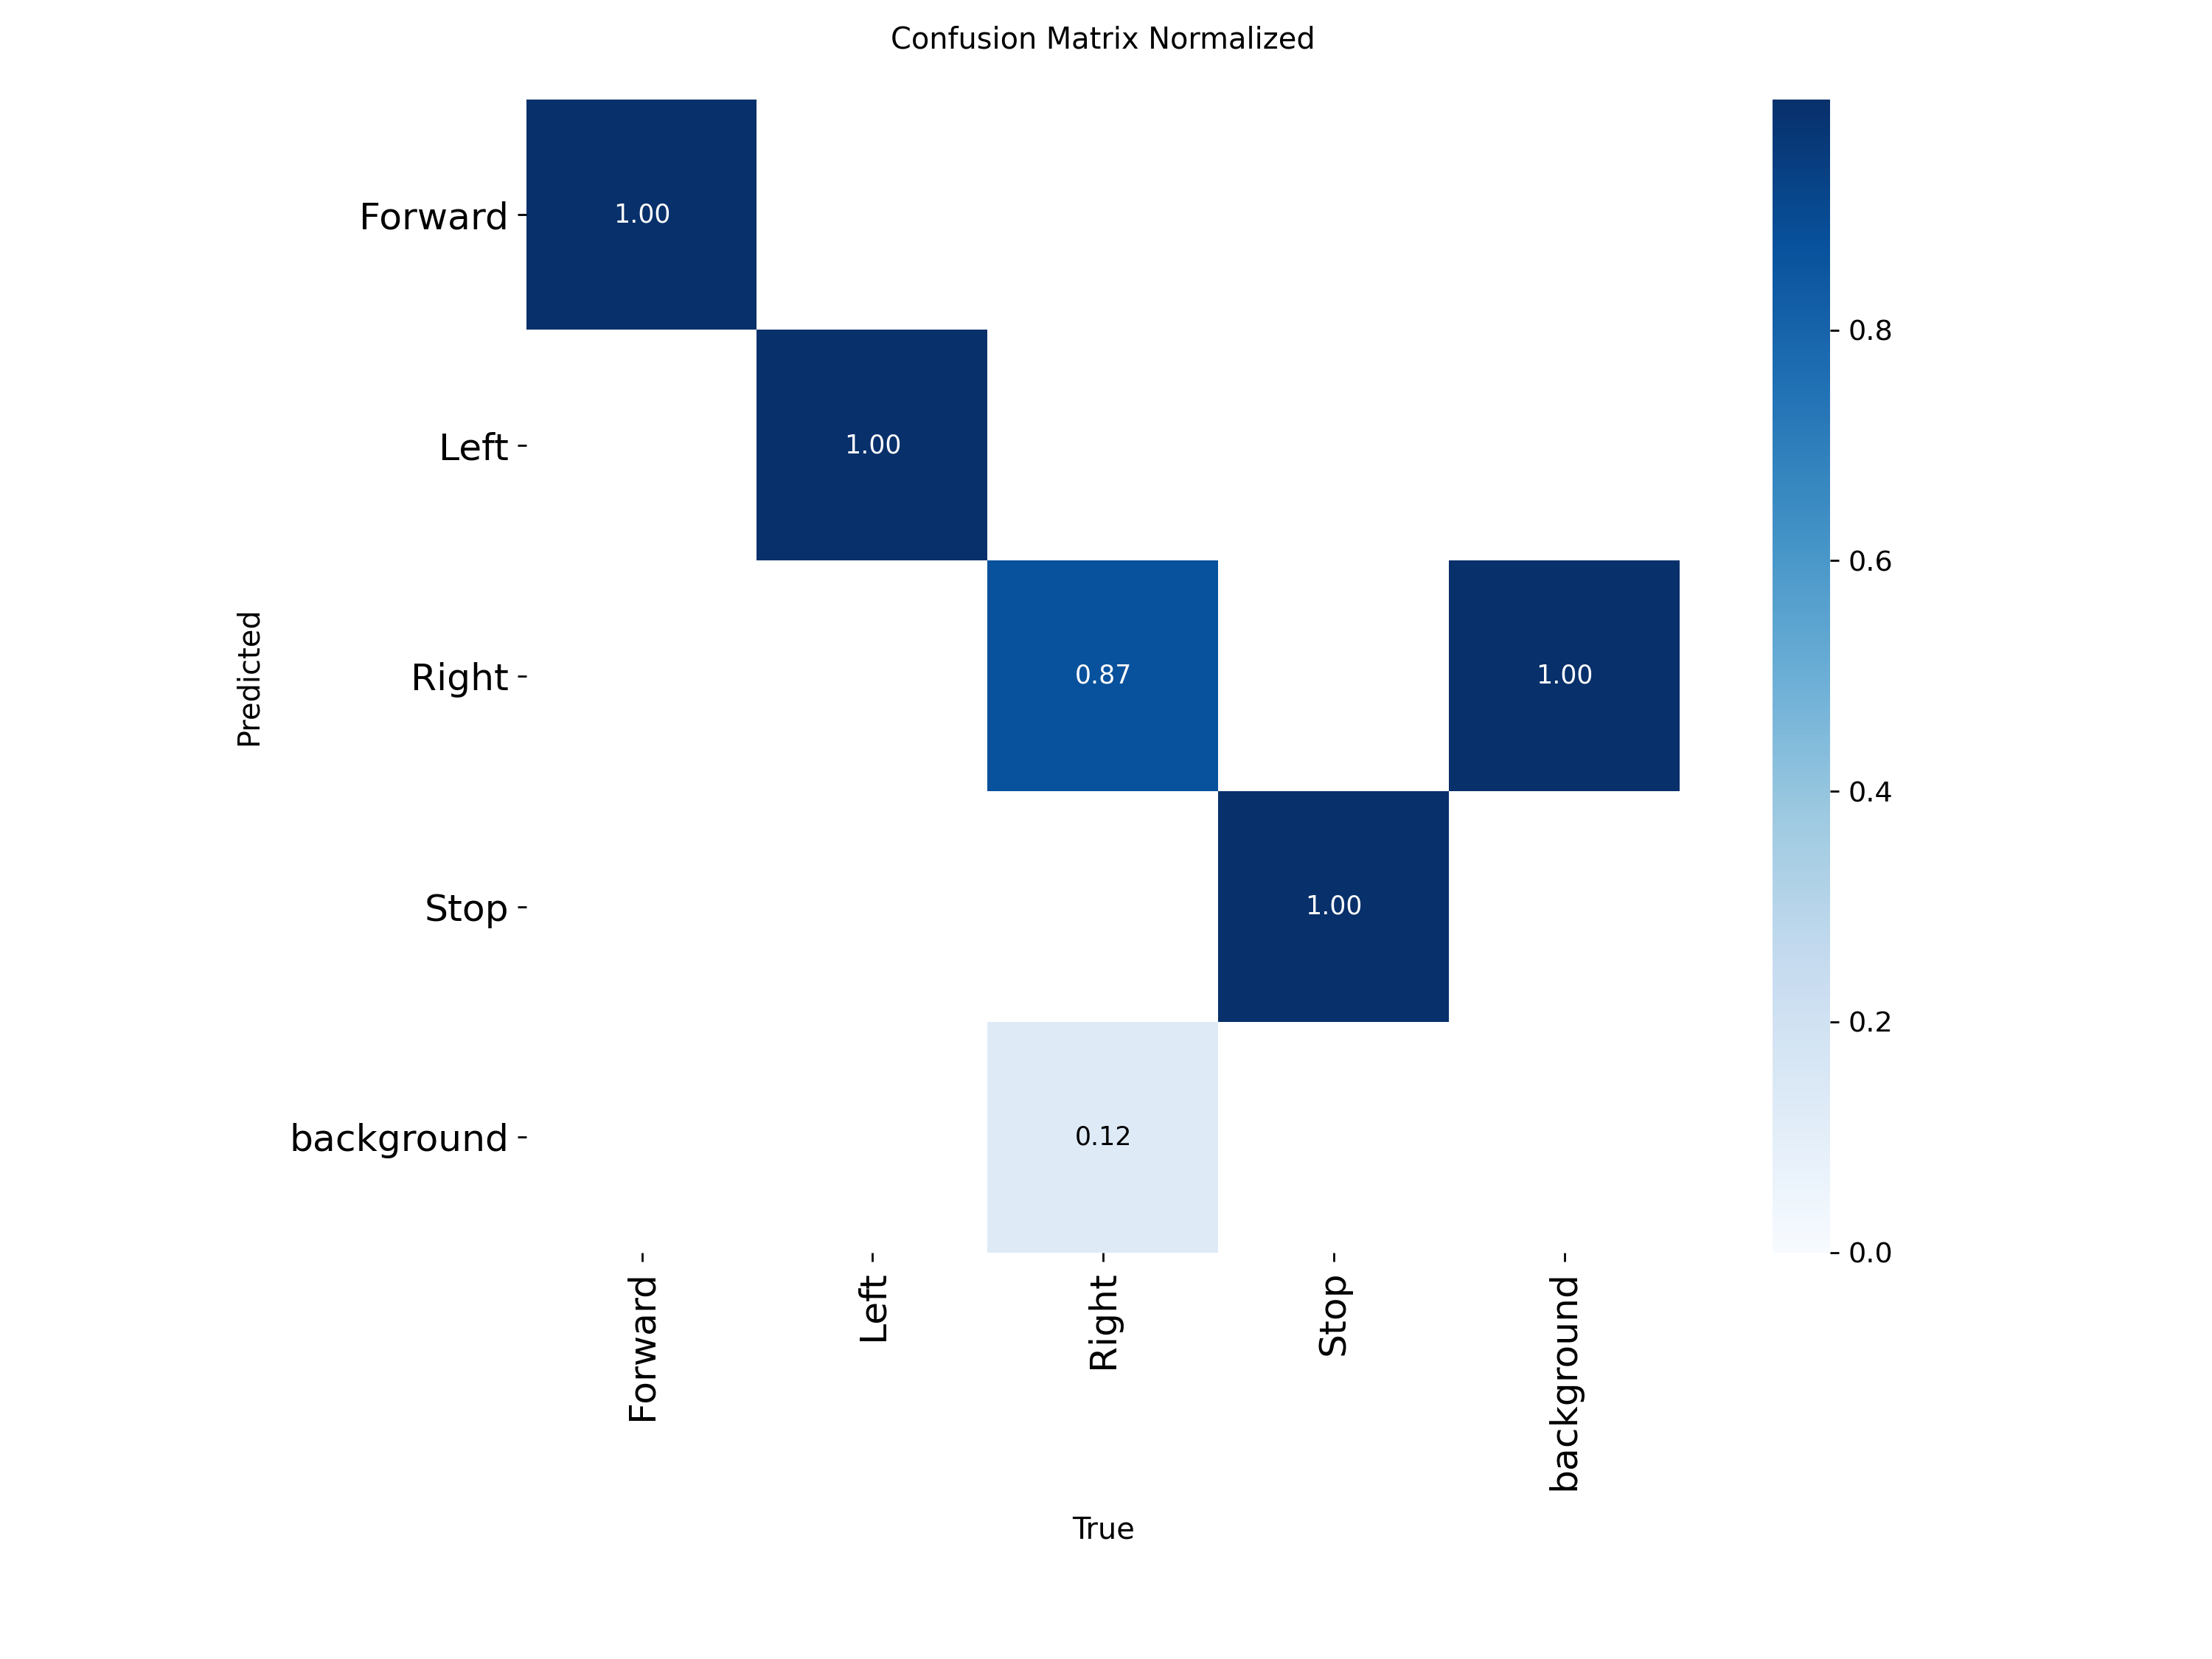
\includegraphics[width=0.75\textwidth]{OAKD/oakd_matrice_confusion.png}
		\caption{Normalised confusion matrix on the validation set}
		\label{fig:oakd-matrice-entrainement}
	\end{figure}
	
	\begin{figure}[H]
		\centering
		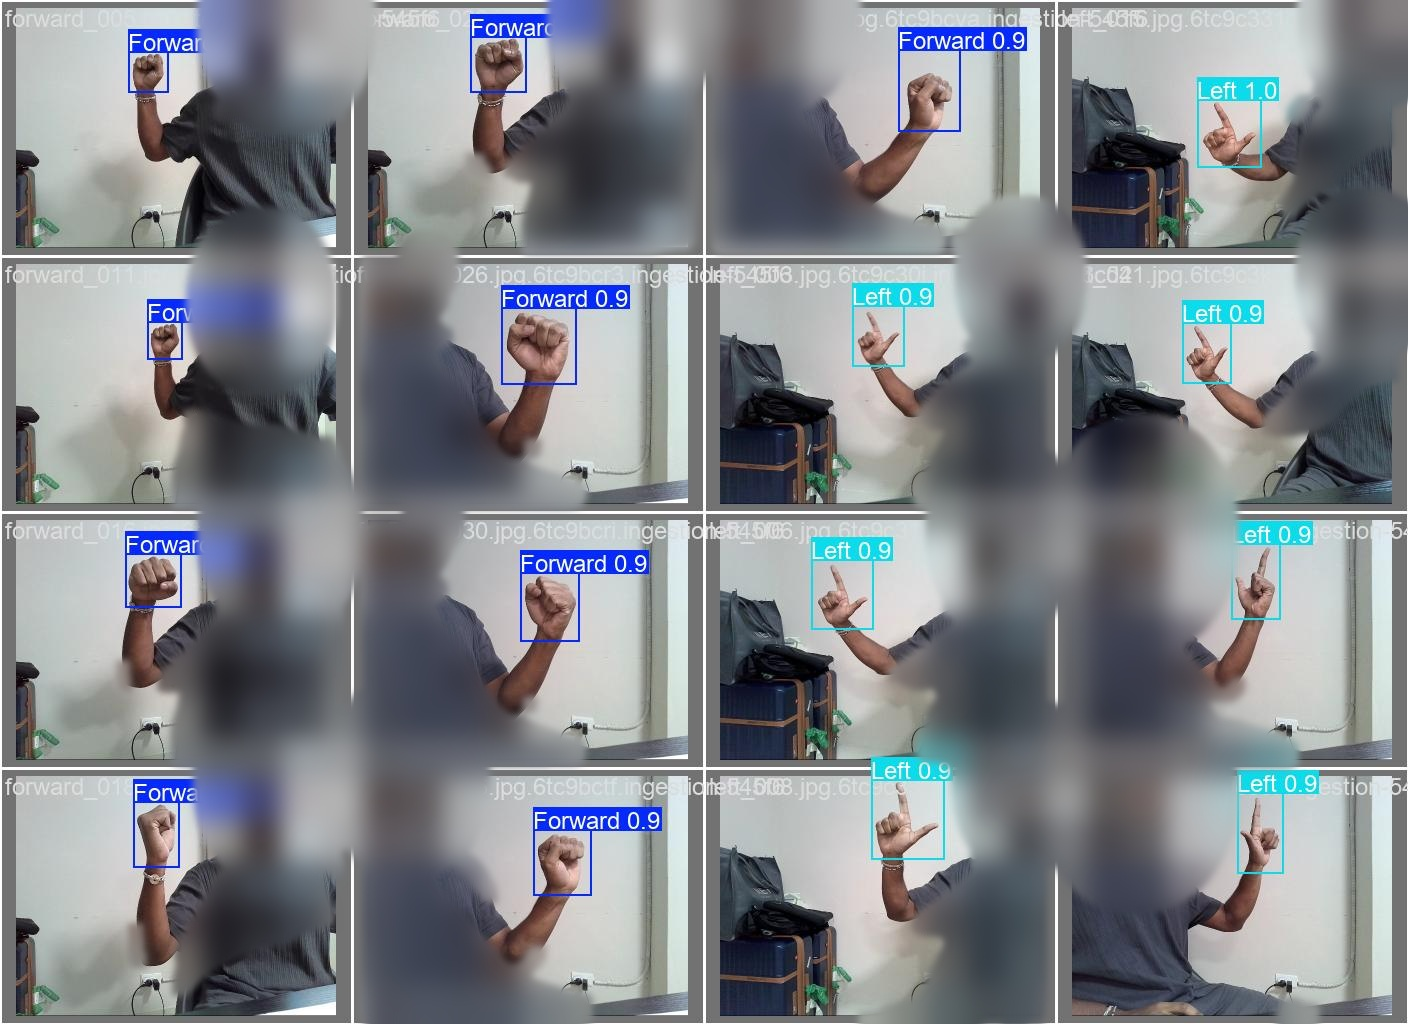
\includegraphics[width=0.85\textwidth]{OAKD/oakd_predictions_validation.jpg}
		\caption{Examples of model predictions on a batch of training images (Forward and Left gestures)}
		\label{fig:oakd-predictions}
	\end{figure}
	
	\subsection*{Export and conversion for the Myriad X chip}
	
	Deployment on the OAK-D Lite requires a three-step conversion chain, specific to the Myriad~X architecture. The trained model (\texttt{best.pt}) is first exported to the ONNX format via \texttt{exporter\_onnx.py} (image size~320, opset~12). This ONNX file is then converted to the \texttt{.blob} format, the proprietary binary format directly executable by the Myriad~X, using the official Luxonis online converter~\cite{luxonis_blobconverter}, with the optimisation parameters \texttt{-scale 255 -reverse\_input\_channels} (pixel normalisation and conversion of the BGR/RGB colour channel order), an 8-bit compilation (\texttt{-ip U8}) and 6 \textit{shaves} (computing units of the Myriad~X allocated to inference).
	
	\begin{figure}[H]
		\centering
		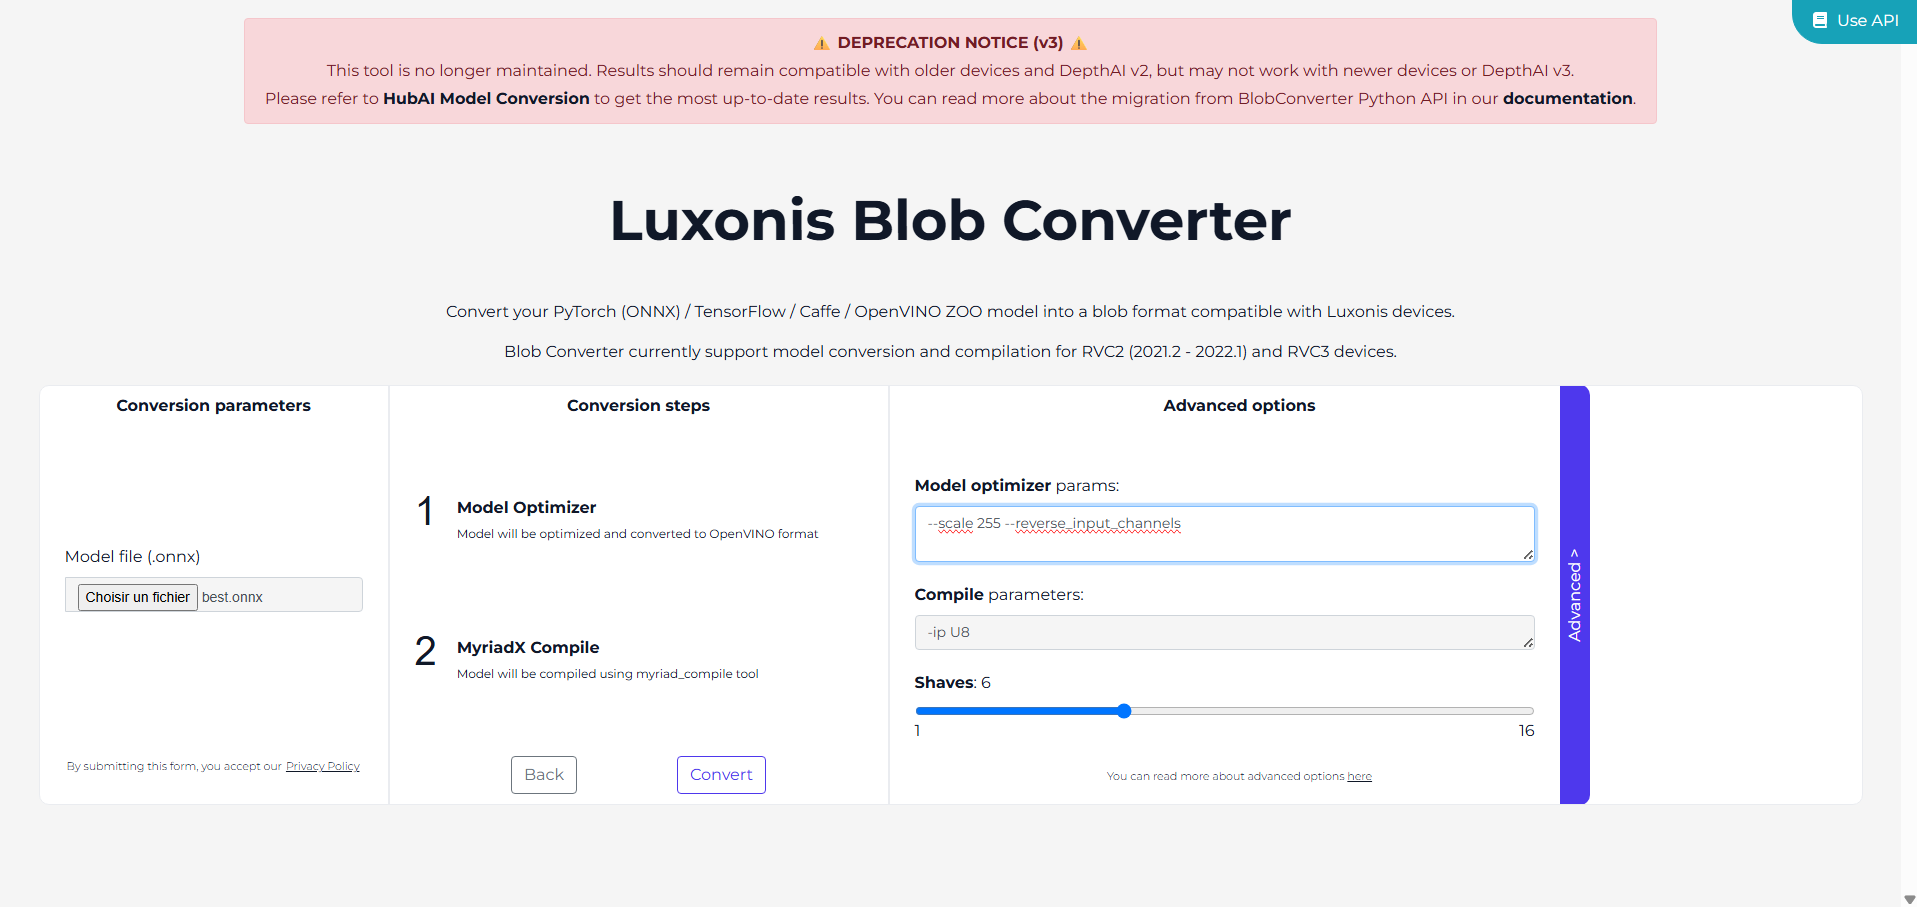
\includegraphics[width=0.9\textwidth]{OAKD/oakd_conversion_blob.png}
		\caption{Conversion of the ONNX model to the \texttt{.blob} format (Luxonis Blob Converter)}
		\label{fig:oakd-conversion}
	\end{figure}
	
	Once the \texttt{best.blob} file is obtained, the \texttt{inspecter\_blob.py} script makes it possible to check, by loading it onto the camera via a minimal DepthAI pipeline, the name, shape and type of its output tensors (\texttt{output0}, of shape $(1, 8, 2100)$), information that is indispensable for correctly writing the decoding of the results on the PC side.
	
	\subsection*{Robot control (\texttt{oakd\_to\_serial.py})}
	
	Unlike the Nicla Vision, the OAK-D Lite requires only a single serial connection, that of the robot: communication with the camera itself is handled natively by the DepthAI SDK via its own protocol (XLink), without a port conflict equivalent to the one encountered with the OpenMV IDE (Section~4.3).
	
	The \texttt{decoder\_yolo()} function decodes the raw output of the neural network, a tensor of shape $(1, 8, 2100)$ representing 2100 candidate boxes, each described by 4 coordinates and 4 class scores. For each frame, the box with the highest score is retained, provided that this score exceeds a confidence threshold (\texttt{CONF\_THRESHOLD}, 0.5). The rest of the control reuses identically the logic already established for the previous solutions: temporal confirmation filtering (\texttt{CONFIRM\_COUNT}, 5 consecutive detections), translation into a JSON command, periodic sending (\texttt{SEND\_INTERVAL}, 150~ms) and software-restart sequence of the robot. An OpenCV window displays live the video stream, the detected bounding box and the recognised gesture.
	
	\subsection*{Validation of control}
	
	Control of the robot by the OAK-D Lite was successfully validated. Figure~\ref{fig:oakd-resultat} shows the Forward gesture detected with a confidence score of 0.90, the corresponding \texttt{forward} command transmitted to the robot, and the returned telemetry confirming the change of mode (\texttt{mode=forward}) and the robot's forward motion.
	
	\begin{figure}[H]
		\centering
		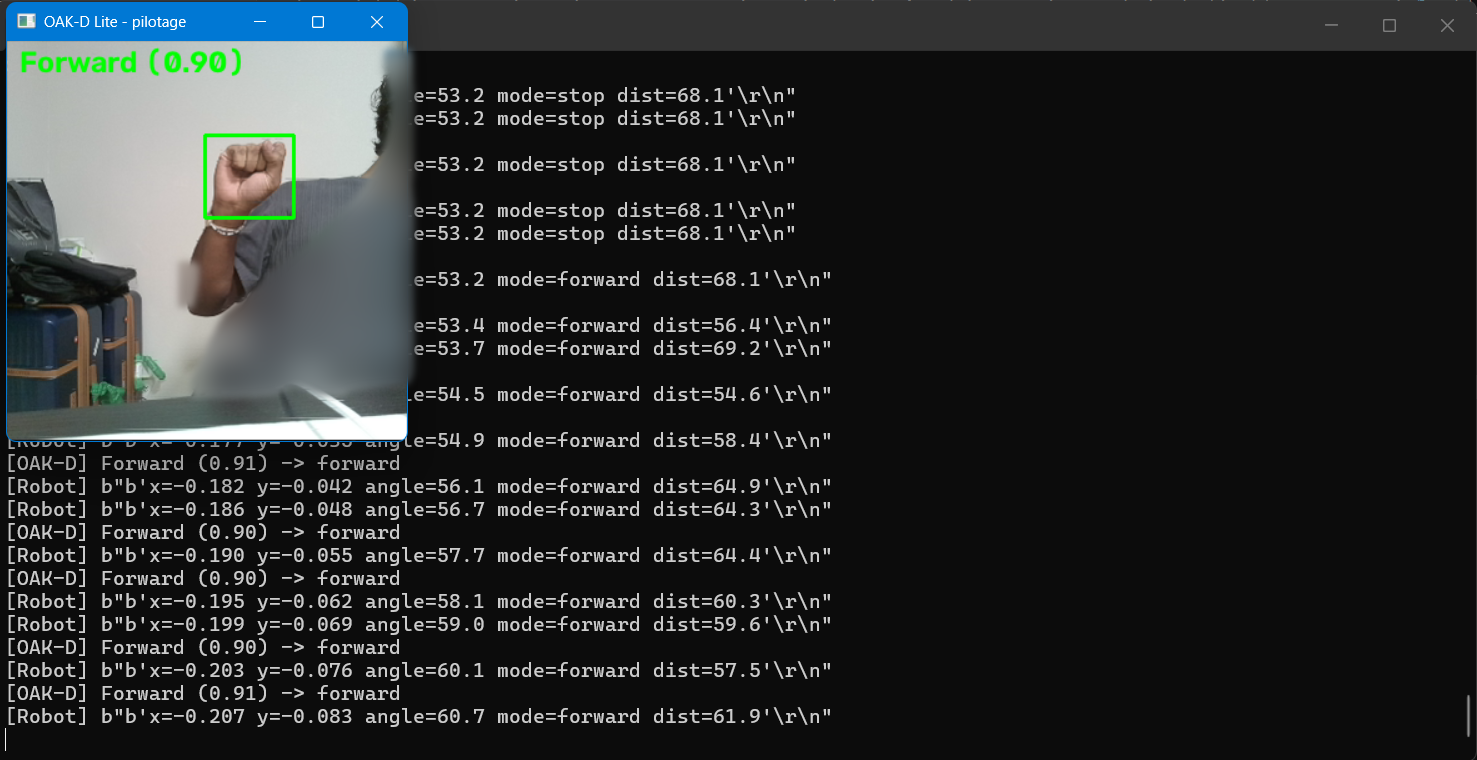
\includegraphics[width=0.85\textwidth]{OAKD/oakd_resultat_pilotage.png}
		\caption{Control of the robot by the OAK-D Lite: video stream, detection and robot terminal}
		\label{fig:oakd-resultat}
	\end{figure}				
	
	\subsection*{Benchmark results}
	
	%=======================================================================
	%	OAK-D Lite latency
	%=======================================================================
	
	\paragraph{Latency:} \mbox{} \\
	Latency was measured using a dedicated script (\texttt{benchmark\_latence\_oakd.py}), which relies on a shared module (\texttt{oakd\_common.py}) grouping together the configuration of the DepthAI pipeline and the YOLOv8 decoding function already presented in Section~4.5 \\ (\texttt{decoder\_yolo()}). To work, these two files must be placed in the same folder as the converted model (\texttt{best.blob}), the latter being loaded by its relative path (\texttt{BLOB\_PATH~=~"best.blob"}).
	
	\textbf{Segment A} exploits a particularity of the DepthAI SDK: each message, whether a captured image or an inference result, carries a sequence number (\texttt{getSequenceNum()}). The \texttt{mesurer\_segment\_a()} function records, for each captured image, the instant of its reception on the PC side in a dictionary indexed by this sequence number. When an inference result carrying the same sequence number is received, the latency is computed as the gap between these two instants, which precisely associates each result with the exact image that produced it, unlike a simple measurement of the interval between two consecutive results. A video window (OpenCV) displays the stream live with the current detection, the \texttt{s} key allowing the measurement to be started at the desired moment (100 measurements are then collected automatically). \textbf{Segment B+C (communication)} reuses, without any modification, the same ping/pong mechanism already used for the four previous solutions.
	
	\begin{table}[H]
		\centering
		\small
		\begin{tabular}{lccccc}
			\toprule
			\textbf{Latency} & \textbf{Mean} & \textbf{Median} & \textbf{Std. dev.} & \textbf{Min} & \textbf{Max} \\
			\midrule
			Segment A (OAK-D Lite) & 42.14~ms & 46.60~ms & 7.10~ms & 30.92~ms & 48.59~ms \\
			Segment B+C (comm.) & 5.37~ms & 3.91~ms & 4.28~ms & 3.18~ms & 20.76~ms \\
			\bottomrule
		\end{tabular}
		\caption{Latency of the OAK-D Lite solution (100 measurements Segment A, 88/100 valid measurements Segment B+C)}
		\label{tab:latence-oakd}
	\end{table}
	
	\begin{figure}[H]
		\centering
		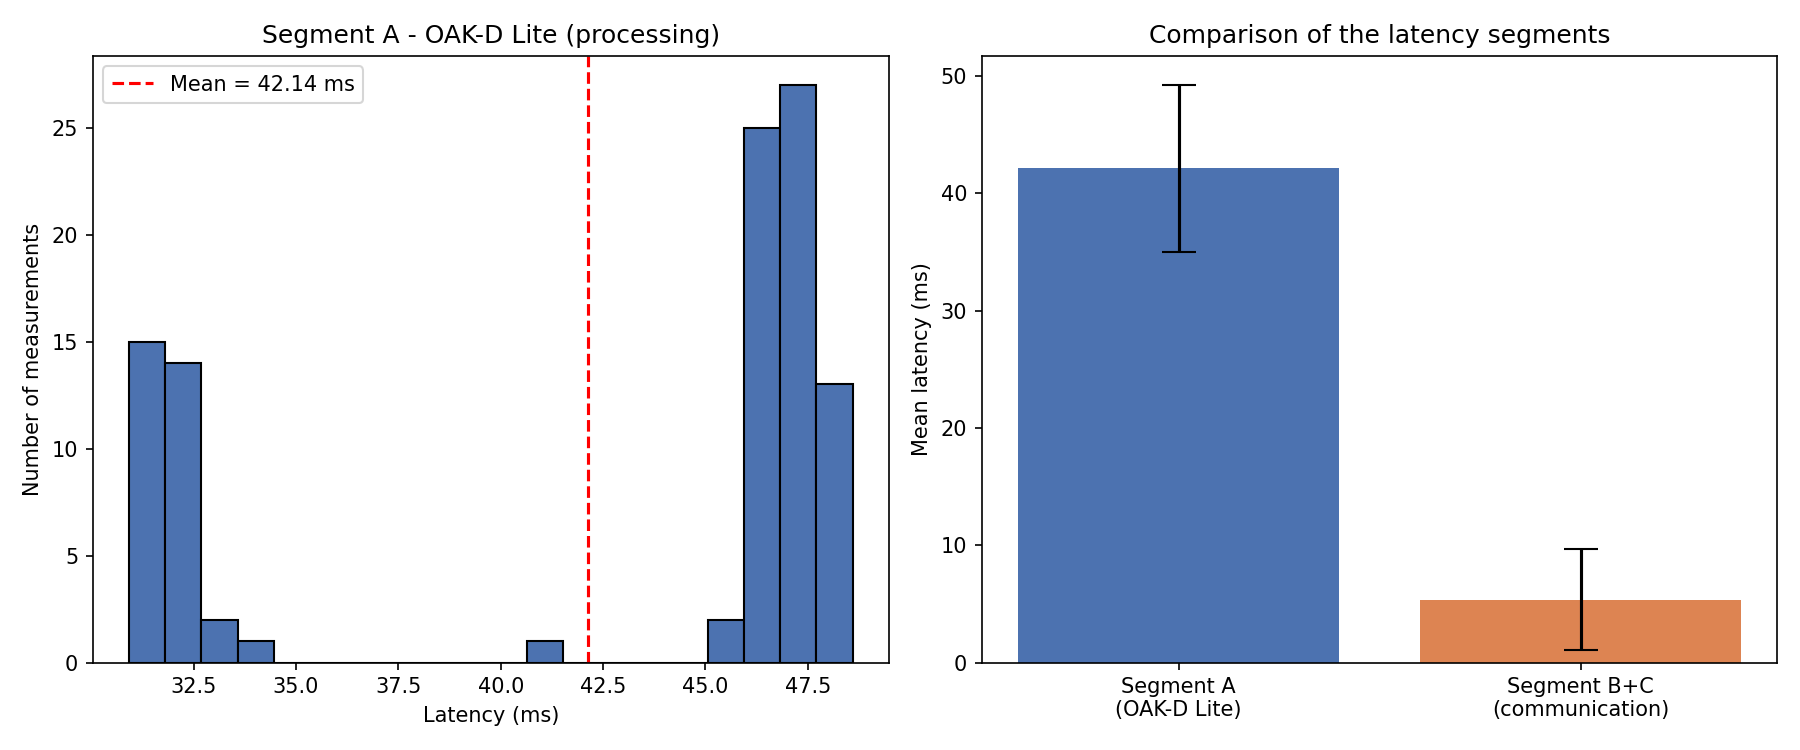
\includegraphics[width=0.95\textwidth]{OAKD/graphique_latence_oakd.png}
		\caption{Distribution of the OAK-D Lite latency: histogram of segment A (left) and comparison of the two segments (right)}
		\label{fig:latence-oakd}
	\end{figure}
	
	\paragraph{Analysis of the results:} \mbox{} \\
	The processing segment (median 46.60~ms) is very markedly higher than that of the four other solutions, consistent with the complexity of the model run: unlike the light internal classification of the HuskyLens or the FOMO model of the Nicla Vision, the OAK-D Lite runs a complete YOLOv8n object-detection model, involving feature extraction over more layers and more costly post-processing.
	
	The histogram on the left (Figure~\ref{fig:latence-oakd}) reveals a markedly \textbf{bimodal} distribution of segment A, with a first group of measurements concentrated around 31 to 33~ms, and a second, larger one, around 46 to 48~ms. This structure is probably explained by a slight desynchronisation between the camera's acquisition frequency and the processing rate of the neural network on the Myriad~X: depending on whether or not a frame has to wait in the queue before being processed, the measured time differs by one full capture cycle. This behaviour, specific to the DepthAI pipeline, also explains the large gap between the mean (42.14~ms, pulled downwards by the fast group) and the median (46.60~ms, more representative of the most frequent case).
	
	The communication segment remains of the same order of magnitude as for the other solutions (median 3.91~ms), with, however, a higher loss (12 pings out of 100 unanswered) than for most of the previous solutions, probably related to the load of the DepthAI pipeline (video processing and continuous inference) running in parallel on the same PC, which can occasionally delay the processing of the serial port on the host side.
	
	The total software latency thus stands at around 47.5~ms on average and 50.5~ms in median, the highest of the five studied solutions, but which nevertheless remains compatible with real-time control of the robot, staying below the human perceptibility threshold for a command delay, generally estimated between 100 and 150~ms.
	
	%=======================================================================
	%	OAK-D Lite FPS
	%=======================================================================
	
	\paragraph{Throughput (FPS):} \mbox{} \\
	Throughput was measured using a dedicated script (\texttt{benchmark\_fps\_oakd.py}), which relies on the same shared module (\texttt{oakd\_common.py}) as the latency benchmark. These two files, as well as the converted model (\texttt{best.blob}), must be placed in the same folder at the time of execution.
	
	The \texttt{mesurer\_fps()} function displays a live video stream (OpenCV window), \\ the \texttt{s} key allowing the measurement to be started at the desired moment, for a fixed duration of 30~seconds (\texttt{DUREE\_MESURE}), of which the first 3 seconds are excluded from the statistics (\texttt{WARMUP\_SEC}). Unlike the throughput of the WebCam, measured on a simple capture loop, this measurement includes the real-time video rendering (OpenCV display with label and score overlaid), in order to reflect the real conditions of use during robot control (Section~4.5), which also displays a continuous video stream. The instantaneous FPS is computed as the inverse of the time elapsed between two consecutive inference results ($\text{FPS} = 1/\Delta t$), and each measurement is classified according to whether a valid detection (score above the confidence threshold) was or was not identified on the corresponding frame.
	
	\begin{table}[H]
		\centering
		\small
		\begin{tabular}{lccccc}
			\toprule
			\textbf{Throughput} & \textbf{n} & \textbf{Mean} & \textbf{Median} & \textbf{Std. dev.} & \textbf{Min / Max} \\
			\midrule
			Overall & 810 & 30.56~FPS & 31.98~FPS & 3.78 & 21.11 / 33.89~FPS \\
			Active detection & 600 & 30.55~FPS & 32.00~FPS & 3.79 & 21.11 / 33.89~FPS \\
			No detection & 210 & 30.58~FPS & 31.96~FPS & 3.74 & 21.29 / 33.81~FPS \\
			\bottomrule
		\end{tabular}
		\caption{Throughput (FPS) of the OAK-D Lite solution with active video rendering, over 27~seconds of useful measurement (810 samples)}
		\label{tab:fps-oakd}
	\end{table}
	
	\begin{figure}[H]
		\centering
		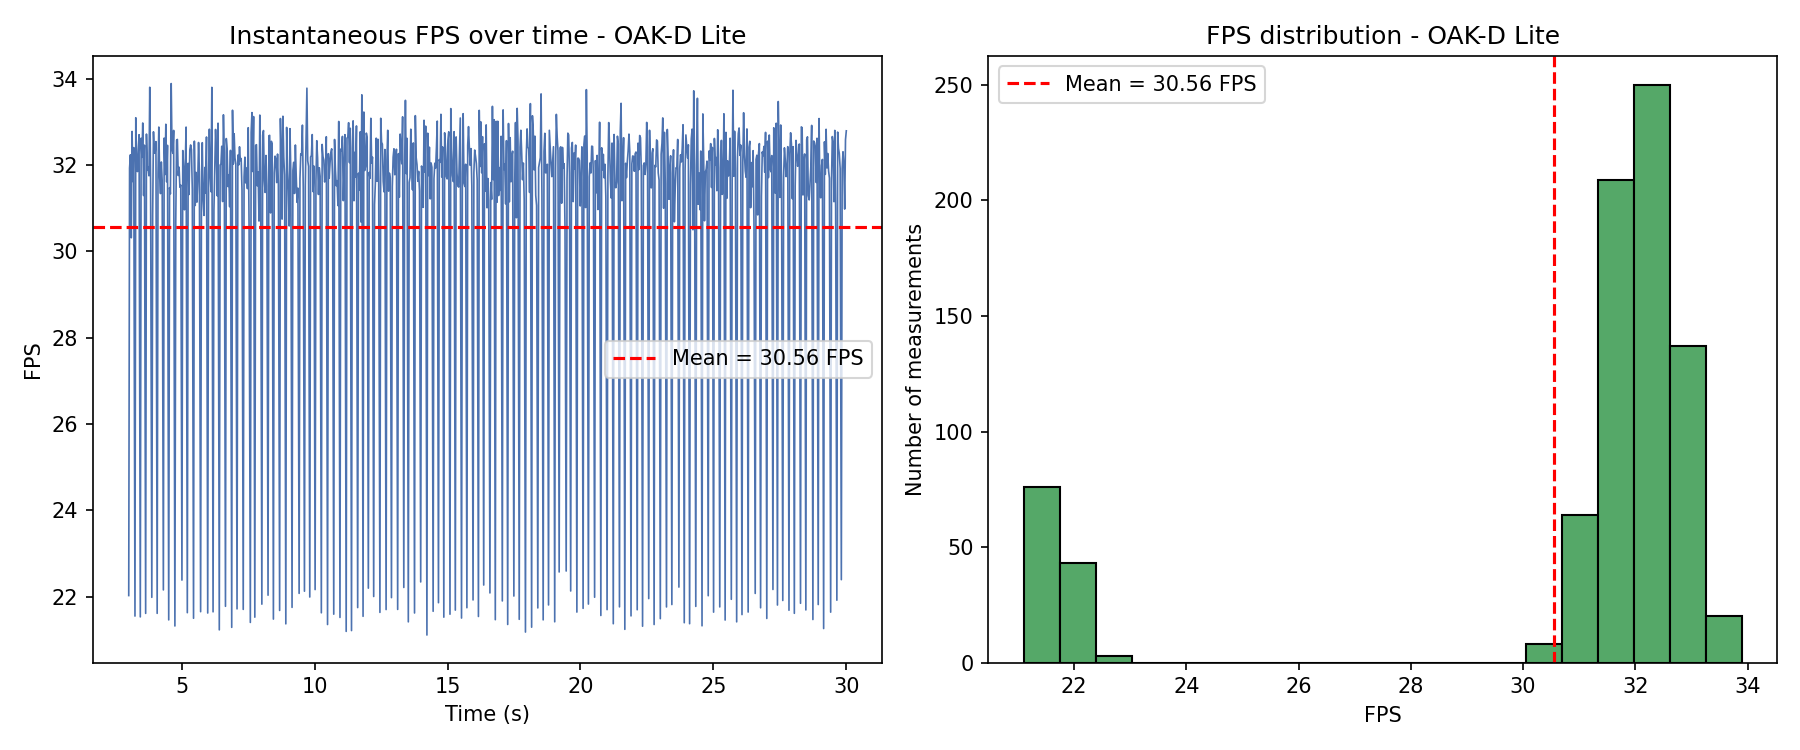
\includegraphics[width=\textwidth]{OAKD/graphique_fps_oakd.png}
		\caption{Throughput (FPS) of the OAK-D Lite with active video rendering: temporal evolution (left) and distribution (right)}
		\label{fig:fps-oakd}
	\end{figure}
	
	\paragraph{Analysis of the results:} \mbox{} \\
	The mean throughput stands at 30.56~FPS, an order of magnitude comparable to that of the WebCam (30.61~FPS, Section~4.1), despite a markedly heavier processing architecture (complete YOLOv8n model on Myriad~X). This result is explained by the fact that the DepthAI pipeline runs the inference directly on the chip, in parallel with the capture, without the PC having to wait for the end of a computation before retrieving the next image.
	
	The distribution (Figure~\ref{fig:fps-oakd}, right) is markedly \textbf{bimodal}: a majority group of measurements concentrated between 31 and 34~FPS, and a second group, minority but regular, around 21 to 23~FPS. The temporal graph (left) shows that this second group does not correspond to a few isolated measurements but to regular periodic oscillations throughout the 27~seconds of useful measurement. This behaviour is probably explained by the rendering cost of the OpenCV video window (\texttt{cv2.imshow}, \texttt{cv2.waitKey}), run at each iteration of the main loop: the inference pipeline on the Myriad~X continues to run at a stable rate, but the time measured on the PC side (which includes the display) varies according to the instantaneous load of the operating system.
	
	As for the previous solutions, the presence of an active detection does not appreciably affect the throughput (30.55~FPS versus 30.58~FPS without detection), confirming that the inference runs at a fixed rate on the chip, independently of the image content.
	
	%=======================================================================
	%	OAK-D Lite confusion matrix
	%=======================================================================
	
	\paragraph{Recognition reliability:} \mbox{} \\
	Reliability was measured using a dedicated script (\texttt{benchmark\_fiabilite\_oakd.py}), which reuses the same manual protocol as the previous solutions: the \texttt{acquerir\_essais()} function displays live the detected gesture as well as the counter of remaining trials for each of the four gestures, and the user validates each trial by pressing a key (\texttt{1}~=~Forward, \texttt{2}~=~Stop, \texttt{3}~=~Left, \texttt{4}~=~Right) corresponding to the gesture they actually intended to make. The script then records the pair (intended gesture, last gesture detected by the YOLOv8n model at that precise instant). Acquisition stops automatically once each of the four gestures has reached 20 trials, i.e. 80 trials in total. The \texttt{construire\_matrice\_confusion()} function then aggregates the trials into a confusion matrix, including a ``none'' column for the trials where no valid detection was present at the moment of validation, then \texttt{generer\_graphique()} produces a graphical representation of it (\textit{heatmap}) with Matplotlib.
	
	\begin{table}[H]
		\centering
		\small
		\begin{tabular}{lccccc}
			\toprule
			\textbf{Intended \textbackslash\ Detected} & \textbf{Forward} & \textbf{Stop} & \textbf{Left} & \textbf{Right} & \textbf{none} \\
			\midrule
			Forward & 19 & 0 & 0 & 0 & 1 \\
			Stop & 0 & 9 & 0 & 0 & 11 \\
			Left & 0 & 0 & 18 & 0 & 2 \\
			Right & 0 & 0 & 0 & 12 & 8 \\
			\bottomrule
		\end{tabular}
		\caption{Confusion matrix of the OAK-D Lite solution (80 trials, 20 per gesture)}
		\label{tab:confusion-oakd}
	\end{table}
	
	\begin{figure}[H]
		\centering
		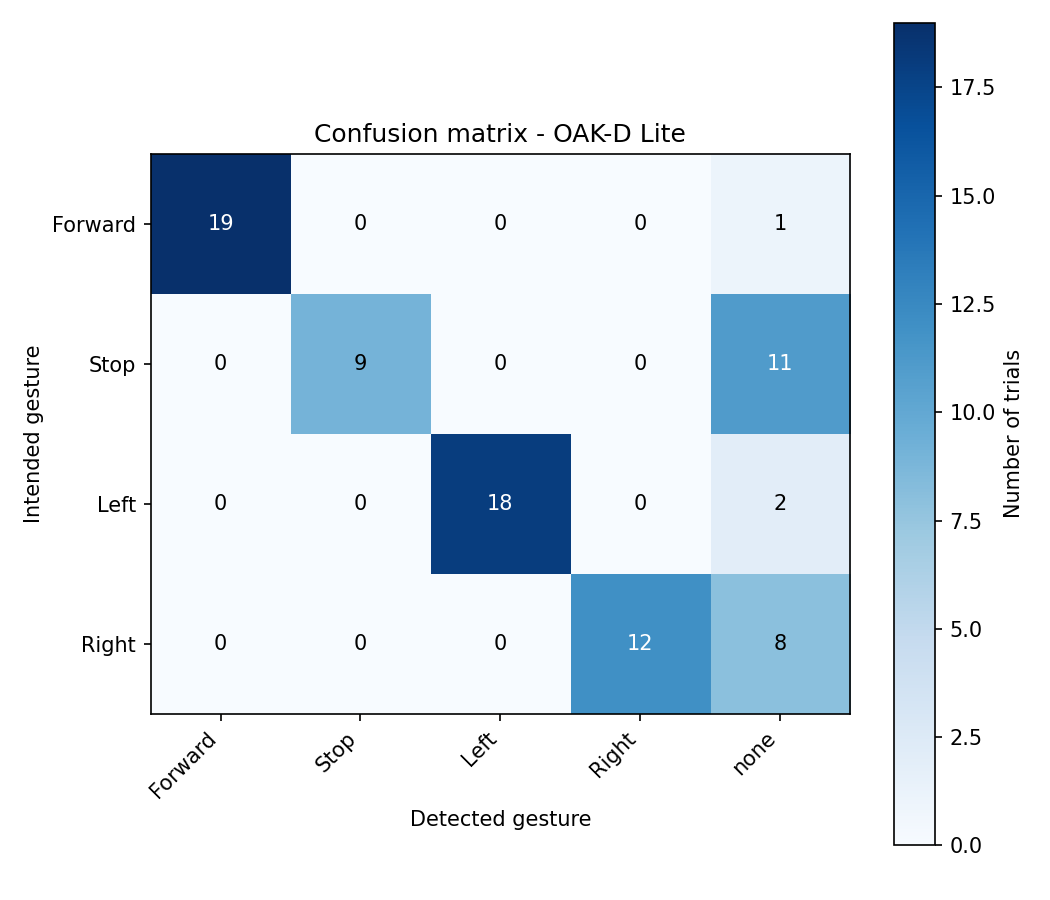
\includegraphics[width=0.75\textwidth]{OAKD/graphique_fiabilite_oakd.png}
		\caption{Confusion matrix of the OAK-D Lite solution (graphical representation)}
		\label{fig:fiabilite-oakd}
	\end{figure}
	
	\paragraph{Analysis of the results:} \mbox{} \\
	The OAK-D Lite solution achieves an overall recognition rate of 72.5\% (58/80), the lowest of the solutions tested so far, despite a mAP50 of 96.6\% obtained during training (Section~4.5). Unlike the HuskyLens or the Nicla Vision, the confusion matrix shows \textbf{no confusion between distinct gestures}: all of the errors correspond to trials classified as ``none'' (no valid detection at the moment of validation), and not to a gesture confused with another.
	
	This result is very contrasted depending on the gesture: Forward (95\%) and Left (90\%) are recognised almost perfectly, while Stop drops to 45\% (11 non-detections out of 20) and Right to 60\% (8 non-detections out of 20). This marked gap with the excellent metrics obtained during training (Section~4.5, where only Right showed a slight weakness at 87\%) suggests that the main cause does not lie in the quality of the model itself, but rather in the \textbf{validation protocol under real conditions}: the fixed confidence threshold (\texttt{CONF\_THRESHOLD}, 0.5) combined with the absence of temporal filtering in this script (unlike the actual control, which applies a confirmation filter over several consecutive detections) makes the measurement sensitive to the exact, often very brief, instant at which the user presses the validation key relative to the moment when the gesture is fully visible and stable in front of the camera.
	
	This result, markedly lower than that of the WebCam (100\%) and of the HuskyLens (86.2\%), illustrates an important methodological limitation to take into account in the final comparative synthesis: the measured reliability depends as much on the test protocol as on the intrinsic quality of the model, a point that distinguishes this measurement from the training reliability presented in Section~4.5.
	
	%=======================================================================
	%	OAK-D Lite consumption
	%=======================================================================
	
	\paragraph{Power consumption:} \mbox{} \\
	As for the four previous solutions, this last metric aimed to measure the electrical consumption of the OAK-D Lite using an INA219 module, placed in series on its power supply, in order to compare its consumption at rest and in active operation. This measurement would have been particularly interesting for this camera: with its three image sensors, its external DRAM memory and its Myriad~X vision processor (up to 4~TOPS), the OAK-D Lite was anticipated, from the preliminary comparative synthesis (Section~2.3), as the most power-hungry solution of the benchmark, without any direct measurement having been able to confirm this hypothesis.
	
	This measurement could, as for the four other solutions, not be carried out, for the same methodological reason: inserting an INA219 module on the camera's power supply requires temporarily cutting a power wire, a modification of the wiring that was not deemed advisable to make without explicit authorisation on hardware lent by the laboratory. This limitation, already set out in Section~4.1, therefore also applies to the OAK-D Lite solution.
	
	\newpage
	
	%----------------------------------------------------------------------
	%	6 RESULTS
	%----------------------------------------------------------------------
	
	\chapter{Results}
	
	%----------------------------------------------------------------------
	%	6.1 Comparative tables
	%----------------------------------------------------------------------
	
	\section{Comparative tables}
	
	This section brings together, for each of the four benchmark metrics, the results already presented individually for each solution in Chapter~4, in order to allow a direct comparison. The OpenMV, whose deployment was blocked by a hardware limitation (Section~4.2), appears in each table with the mention ``not measurable'', to recall its status rather than by omission.
	
	\subsection*{Latency}
	
	Table 6.1 details, for each solution, the latency per segment (vision-processing segment, and communication segment to the robot), as well as the total software latency.
	
	\begin{table}[H]
		\centering
		\small
		\renewcommand{\arraystretch}{1.2}
		\begin{tabularx}{\textwidth}{|l|X|X|X|X|}
			\hline
			\textbf{Solution} & \textbf{Vision segment (median)} & \textbf{Comm. segment (median)} & \textbf{Total (median)} & \textbf{Total (mean)} \\
			\hline
			WebCam + MediaPipe & 25.90~ms & 3.92~ms & 29.82~ms & 31.76~ms \\
			\hline
			OpenMV & \multicolumn{4}{c|}{Not measurable} \\
			\hline
			Nicla Vision & 64.76~ms & 4.02~ms & 68.78~ms & 104.00~ms \\
			\hline
			HuskyLens & 2.01~ms & 3.84~ms & 5.85~ms & 8.00~ms \\
			\hline
			OAK-D Lite & 46.60~ms & 3.91~ms & 50.51~ms & 47.51~ms \\
			\hline
		\end{tabularx}
		\caption{Comparison of the latency of the five solutions}
		\label{tab:comparatif-latence}
	\end{table}
	
	\noindent\textit{Comment:} The HuskyLens shows the lowest latency, followed by the WebCam, then the OAK-D Lite and finally the Nicla Vision, the slowest. The communication segment remains appreciably identical from one solution to another (between 3.84 and 4.02~ms), which is expected since the code embedded on the robot was never modified from one solution to another (Section~3.2). The bulk of the gap between the solutions therefore comes from the vision-processing segment, specific to each architecture.
	
	\subsection*{Throughput (FPS)}
	
	\begin{table}[H]
		\centering
		\small
		\renewcommand{\arraystretch}{1.2}
		\begin{tabularx}{\textwidth}{|l|X|X|X|}
			\hline
			\textbf{Solution} & \textbf{Mean throughput} & \textbf{Median throughput} & \textbf{Std. dev.} \\
			\hline
			WebCam + MediaPipe & 30.61~FPS & 31.62~FPS & 3.63 \\
			\hline
			OpenMV & \multicolumn{3}{c|}{Not measurable} \\
			\hline
			Nicla Vision & 11.82~FPS & 12.82~FPS & 4.45 \\
			\hline
			HuskyLens & 445.10~FPS & 492.08~FPS & 132.42 \\
			\hline
			OAK-D Lite & 30.56~FPS & 31.98~FPS & 3.78 \\
			\hline
		\end{tabularx}
		\caption{Comparison of the throughput (FPS) of the five solutions}
		\label{tab:comparatif-fps}
	\end{table}
	
	\noindent\textit{Comment:} The WebCam and the OAK-D Lite show an almost identical throughput (around 31 to 32~FPS), consistent with the native acquisition frequency of an image sensor at moderate resolution. The much higher throughput of the HuskyLens (492~FPS in median) must be interpreted with caution: as already noted in Section~4.4, this value reflects the speed at which the PC queries the serial port rather than an actual refresh rate of the camera's internal recognition. The Nicla Vision shows the lowest throughput of the four measurable solutions (12.82~FPS), consistent with the markedly longer cycle time observed in the latency segment.
	
	\subsection*{Recognition reliability}
	
	\begin{table}[H]
		\centering
		\small
		\renewcommand{\arraystretch}{1.2}
		\begin{tabularx}{\textwidth}{|l|X|X|}
			\hline
			\textbf{Solution} & \textbf{Recognition rate} & \textbf{Correct trials} \\
			\hline
			WebCam + MediaPipe & 100.0\% & 80/80 \\
			\hline
			OpenMV & \multicolumn{2}{c|}{Not measurable} \\
			\hline
			Nicla Vision & 83.8\% & 67/80 \\
			\hline
			HuskyLens & 86.2\% & 69/80 \\
			\hline
			OAK-D Lite & 72.5\% & 58/80 \\
			\hline
		\end{tabularx}
		\caption{Comparison of the recognition reliability of the five solutions}
		\label{tab:comparatif-fiabilite}
	\end{table}
	
	\noindent\textit{Comment:} The WebCam is the only solution to achieve perfect reliability. The three measurable smart cameras rank in the reverse order of their on-board computing power: the HuskyLens (the simplest architecture) comes ahead of the Nicla Vision, itself ahead of the OAK-D Lite (the most advanced architecture); this counter-intuitive result will be discussed in more detail in Section~5.2.
	
	\subsection*{Power consumption}
	
	\begin{table}[H]
		\centering
		\small
		\renewcommand{\arraystretch}{1.2}
		\begin{tabularx}{\textwidth}{|l|X|X|}
			\hline
			\textbf{Solution} & \textbf{Consumption at rest} & \textbf{Active consumption} \\
			\hline
			WebCam + MediaPipe & \multicolumn{2}{c|}{Not measured} \\
			\hline
			OpenMV & \multicolumn{2}{c|}{Not measurable} \\
			\hline
			Nicla Vision & \multicolumn{2}{c|}{Not measured} \\
			\hline
			HuskyLens & \multicolumn{2}{c|}{Not measured} \\
			\hline
			OAK-D Lite & \multicolumn{2}{c|}{Not measured} \\
			\hline
		\end{tabularx}
		\caption{Comparison of the power consumption of the five solutions}
		\label{tab:comparatif-consommation}
	\end{table}
	
	\noindent\textit{Comment:} None of the five solutions could be measured on this criterion, for the common methodological reason set out in Section~4.1 (hardware lent by the laboratory, wiring modification not authorised). This limitation therefore applies uniformly and does not introduce any bias between the compared solutions.
	
	\subsection*{Synthesis of the four metrics}
	
	Table 6.5 brings together, in a single view, the median results of the four metrics for all five solutions.
	
	\begin{table}[H]
		\centering
		\small
		\renewcommand{\arraystretch}{1.2}
		\begin{tabularx}{\textwidth}{|l|X|X|X|X|}
			\hline
			\textbf{Solution} & \textbf{Total latency} & \textbf{Throughput} & \textbf{Reliability} & \textbf{Consumption} \\
			\hline
			WebCam + MediaPipe & 29.82~ms & 31.62~FPS & 100.0\% & Not measured \\
			\hline
			OpenMV & Not measurable & Not measurable & Not measurable & Not measurable \\
			\hline
			Nicla Vision & 68.78~ms & 12.82~FPS & 83.8\% & Not measured \\
			\hline
			HuskyLens & 5.85~ms & 492.08~FPS & 86.2\% & Not measured \\
			\hline
			OAK-D Lite & 50.51~ms & 31.98~FPS & 72.5\% & Not measured \\
			\hline
		\end{tabularx}
		\caption{Comparative synthesis of the five solutions across the four benchmark metrics}
		\label{tab:synthese-resultats}
	\end{table}
	
	\noindent\textit{Comment:} This synthesis table highlights that no solution dominates simultaneously across the three measurable metrics: the HuskyLens wins on latency and throughput but not on reliability, the WebCam wins on reliability but remains behind the HuskyLens on latency, while the OAK-D Lite, despite the highest computing power of the benchmark (Section~2.3), does not stand out on any of the three metrics. This absence of a universally dominant solution will be at the heart of the critical analysis and the recommendations presented in the following subsections.
	
	%----------------------------------------------------------------------
	%	6.2 Critical analysis of the 5 solutions
	%----------------------------------------------------------------------
	
	\section{Critical analysis of the 5 solutions}
	
	This section offers a critical reading of the results presented in Section~5.1, solution by solution, then through several cross-cutting observations that run across the whole benchmark. It notably confronts the predictions formulated from the datasheets alone (Section~2.3) with the results actually measured, in order to answer the problem posed in Section~1.2.
	
	\subsection*{WebCam + MediaPipe}
	
	The WebCam stands out as the most balanced solution of the benchmark: perfect reliability (100\%), the second lowest total latency (29.82~ms), and a stable throughput consistent with the sensor's native rate (31.62~FPS). This result confirms the prediction of Section~2.3, which anticipated good reliability driven by the robustness of MediaPipe. Its weak point remains structural rather than measured: it is the only one of the five solutions to depend entirely on a PC to operate, with no autonomous processing capacity.
	
	\subsection*{OpenMV}
	
	The deployment failure of the OpenMV Cam M7, documented in detail in Section~4.2, removes this solution from any quantified comparison. This result nevertheless remains significant with respect to the problem posed: it shows that the choice of the precise hardware of a smart camera, beyond its general category, can be enough to make an embedded processing architecture completely unusable, independently of the quality of the trained model.
	
	\subsection*{Nicla Vision}
	
	The Nicla Vision shows the highest total latency of the benchmark (68.78~ms in median) and the lowest throughput (12.82~FPS), despite a microcontroller markedly more powerful than that of the OpenMV M7. This result partly contradicts the prediction of Section~2.3, which anticipated an advantage related to its higher computing power; in practice, it is the complexity of the model run (FOMO object detection) rather than the raw power of the microcontroller that dominates the cycle time. Its reliability (83.8\%) remains acceptable, but weakened by the software instability of the OpenMV firmware (Section~4.3), which also prevented a benchmark measurement as long and stable as for the other solutions.
	
	\subsection*{HuskyLens}
	
	The HuskyLens obtains the best results on latency (5.85~ms) and, with the methodological caveat already set out (Section~4.4), on throughput. It thus confirms the prediction of Section~2.3, which relied on the simplicity of its classification algorithm rather than on raw computing power to explain its speed. Its reliability (86.2\%) nevertheless remains behind that of the WebCam, with a notable tendency to classify uncertain trials in the Stop class rather than to reject them, a behaviour that is not necessarily representative of a confusion between visually close gestures.
	
	\subsection*{OAK-D Lite}
	
	The OAK-D Lite illustrates the most counter-intuitive result of the benchmark. Despite the highest on-board computing power (4~TOPS) and the best performance obtained during training among the embedded solutions (mAP50 of 96.6\%, Section~4.5), it shows both a high latency (50.51~ms, the second slowest) and the lowest reliability of the benchmark under real conditions (72.5\%). This double result directly invalidates the optimistic prediction made in Section~2.3 about this solution.
	
	The gap between the two metrics (excellent mAP50 during training, low recognition rate in real use) is largely explained by a difference in protocol rather than by the model itself: unlike the actual control script of the OAK-D Lite (Section~4.5), which applies temporal confirmation filtering, the reliability-measurement script (Section~4.5, ``Recognition reliability'' subsection) evaluates a single instantaneous detection, with no tolerance margin on the exact moment of the user's key press. This result is a reminder that a more complex and more powerful architecture is not necessarily synonymous with better overall performance, the way it is used under real conditions weighing at least as much as its raw computing power.
	
	\subsection*{Cross-cutting observations}
	
	\paragraph{Raw computing power does not predict overall performance:} \mbox{} \\
	The ranking of the five solutions on latency and reliability at no point follows the ranking of their on-board computing power established in Section~2.3. The HuskyLens, the least powerful of the four smart cameras, obtains the lowest latency; the OAK-D Lite, the most powerful, obtains the lowest reliability under real conditions. This result confirms that the complexity of the model run (simple classification versus full object detection) and the quality of the usage protocol weigh more on perceived performance than the raw power of the hardware.
	
	\paragraph{A trade-off between processing autonomy and software maturity:} \mbox{} \\ 
	The two solutions that required the heaviest intervention on the embedded software side (OpenMV, definitively blocked, and Nicla Vision, functional but unstable) share the same original firmware (OpenMV), suggesting that the maturity of the software ecosystem around a board weighs at least as much as its hardware characteristics in the feasibility of an embedded vision project. Conversely, the HuskyLens (a closed device, with no inference code to write) and the OAK-D Lite (an actively maintained DepthAI SDK) both allowed a functional deployment without any major software blockage, despite very different internal architectures.
	
	\paragraph{A gradient of implementation complexity:} \mbox{} \\ 
	The five solutions also differ in the complexity of the path required to reach a deployed model: 
	\begin{itemize}
		\item the HuskyLens requires no model writing at all (integrated incremental training, Section~4.4); 
		\item the WebCam requires no training at all (geometric logic on the MediaPipe landmarks, Section~4.1); 
		\item the OpenMV and the Nicla Vision require Edge Impulse training and a firmware deployment (Parts~5.4 and~5.5); 
		\item the OAK-D Lite, finally, imposes the longest chain (labelling, external Ultralytics training, ONNX export, \texttt{.blob} conversion, Section~4.5). 
	\end{itemize} 
	This increasing complexity did not translate, in this project, into any proportional final performance gain.
	
	\paragraph{A dependence on the PC that persists despite the embedded intelligence:} \mbox{} \\ 
	While four of the five solutions use the PC only as a simple command relay while the robot is operating, none achieves complete end-to-end autonomy: training, deployment and, for the Nicla Vision and the OAK-D Lite, the reconstruction of the communication protocol specific to each architecture, all systematically require a PC upstream. Only the HuskyLens reduces this dependence to its minimum, since training can in theory be carried out directly on the device, without a PC.
	
	\newpage
	
	%----------------------------------------------------------------------
	%	6.3 Recommendations
	%----------------------------------------------------------------------
	
	\section{Recommendations}
	
	The central observation of Section~5.2, the absence of a universally dominant solution, invites differentiated recommendations according to the priority criterion targeted by a given application, rather than a single ranking. Table~\ref{tab:recommandations} summarises these recommendations, detailed afterwards criterion by criterion.
	
	\begin{table}[H]
		\centering
		\small
		\renewcommand{\arraystretch}{1.3}
		\begin{tabularx}{\textwidth}{|l|X|}
			\hline
			\textbf{Priority criterion} & \textbf{Recommended solution} \\
			\hline
			Pure responsiveness (minimal latency) & HuskyLens \\
			\hline
			Detection reliability & WebCam + MediaPipe \\
			\hline
			Autonomy from a PC & HuskyLens \\
			\hline
			Simplicity and speed of implementation & WebCam + MediaPipe \\
			\hline
			Ability to evolve towards more complex vision tasks & OAK-D Lite \\
			\hline
		\end{tabularx}
		\caption{Recommendations according to the priority criterion of the target application}
		\label{tab:recommandations}
	\end{table}
	
	\paragraph{For maximum responsiveness:} \mbox{} \\  
	The HuskyLens stands out with the lowest total latency of the benchmark (5.85~ms in median, Section~5.1). This result must nevertheless be qualified by the confirmation delay added by the anti-false-positive filtering (Section~4.4), not counted in this raw measurement, but which applies in a comparable way to the other embedded solutions.
	
	\paragraph{For maximum reliability:} \mbox{} \\ 
	The WebCam remains the only choice showing perfect reliability (100\%, Section~5.1). This result comes, however, with a total dependence on a PC while operating, a trade-off to accept if reliability takes precedence over hardware autonomy.
	
	\paragraph{For maximum autonomy from a PC:} \mbox{} \\ 
	The HuskyLens stands out again, since it is the only one of the five solutions whose training can, in theory, be carried out entirely on the device, without a PC (Section~5.2). The four other solutions, including those that use the PC only as a simple command relay while operating, all require a PC during the training or model-deployment phase.
	
	\paragraph{For a quick implementation, notably in a prototyping or teaching context:} \mbox{} \\ 
	The WebCam remains the most accessible solution, requiring neither additional hardware nor a training phase (Section~4.1). The HuskyLens is a good alternative if an embedded solution is required, its incremental button-based training avoiding any writing of inference code (Section~4.4).
	
	\paragraph{For an application requiring richer vision than simple gesture recognition:} \mbox{} \\ 
	Despite its lowest results on the reliability measured in this project, the OAK-D Lite remains the only solution capable of running modern and complex object-detection architectures (Section~2.2.5), with the best performance obtained during training in the benchmark (mAP50 of 96.6\%, Section~4.5). Its results under real conditions seem more related to the test protocol used (Section~5.2) than to an intrinsic limitation of the hardware, which suggests a significant margin for improvement with a better-suited usage protocol (temporal filtering, as for the actual control of the robot).
	
	\paragraph{Case to avoid:} \mbox{} \\ 
	The OpenMV Cam M7, in its tested configuration (OV7725-M7 module, without an NPU or external RAM), is not recommended for this type of application. The blockage encountered (Section~4.2) appears to be hardware rather than software, and therefore cannot be worked around without changing camera model.
	
	\medskip
	
	Ultimately, the choice of an embedded vision solution for the gesture-based control of a robot depends less on an absolute performance ranking than on an explicit trade-off between responsiveness, reliability, autonomy and implementation complexity, each of the studied solutions occupying a distinct position on these four axes, without any one of them dominating simultaneously.
	
	\newpage
	
	%----------------------------------------------------------------------
	%	7 DIFFICULTIES ENCOUNTERED AND SOLUTIONS APPLIED
	%----------------------------------------------------------------------
	
\chapter{Difficulties specific to the five solutions}
	\section*{Difficulties related to the integration of the five camera solutions}
	
	Several difficulties recurred, in various forms, throughout the integration of the five vision solutions.
	
	\begin{itemize}
		\item \textbf{Robot restart.} The first blockage encountered, during the integration of the WebCam (Section~4.1), was due to the robot remaining stuck at the interactive prompt after an editing session, without running \texttt{code.py}. The software-restart sequence developed on that occasion was then systematically reused, without modification, for the four following solutions.
		\item \textbf{Incorrect hardware identification.} The HuskyLens (Section~4.4) was not detected on any serial port until the erroneous hypothesis of a CH340 USB-serial chip was ruled out in favour of the CP2102N chip actually present, requiring the installation of a specific driver.
		\item \textbf{Documented bugs of third-party libraries.} Several solutions were affected by behaviours not conforming to their official documentation: the \texttt{learned()} method of the HuskyLens library (Section~4.4), or a version regression in MediaPipe making a whole module inaccessible (Section~4.1). In both cases, the solution consisted in identifying the faulty version or the actual behaviour of the function, rather than looking for an error in the project code itself.
		\item \textbf{Hardware limitation that could not be worked around.} The OpenMV Cam M7 (Section~4.2) is the only solution of the benchmark where none of the six correction avenues attempted made it possible to resolve the blockage, leading to the conclusion of a hardware limitation of the board rather than a software bug.
		\item \textbf{Software instability during prolonged operation.} The Nicla Vision (Section~4.3) presented a random crash after several tens of seconds to a few minutes of operation, requiring the benchmark scripts to be designed with a safety time limit rather than a simple measurement counter, so as never to remain blocked indefinitely.
		\item \textbf{Gap between training validation and validation under real conditions.} The reliability measurement of the OAK-D Lite (Section~4.5) revealed a large gap with the metrics obtained during training, not because of a flaw in the model, but because of a difference in protocol between the isolated measurement and the temporal filtering used in actual control (Section~5.2).
	\end{itemize}
	
	\section*{File corruption during transfer}
	
	When resuming the benchmark tests, the files \texttt{robot.py}, \texttt{pio\_encoder.py} and \texttt{pid\_controller.py}, initially provided by the laboratory and already presented in Section~3.1, turned out to have lost all of their Python indentation, causing an \\ \texttt{IndentationError} that prevented the robot from starting. This corruption, probably caused by a copy-paste from a medium that altered the original indentation, was not detectable by simply reading the code in a classic text editor. The correction consisted in reconstructing the correct indentation of the three files from the business logic already documented, then checking that the robot worked correctly before continuing the measurements.
	
\chapter*{Conclusion}
\addcontentsline{toc}{chapter}{Conclusion}
	
	
	
	This internship, initially oriented towards a complex gesture-control architecture (ROS2, Turtlebot~3), was reoriented towards a more experimental problem: comparing five embedded vision solutions for the gesture-based control of a robot, according to a common benchmark protocol (latency, throughput, reliability, consumption).
	
	\medskip
	
	Four of the five solutions led to a usable result, only the OpenMV Cam M7 having been blocked by a hardware limitation. The main observation is that no solution dominates across all of the criteria: the HuskyLens is the most responsive, the WebCam the most reliable, while the OAK-D Lite, despite the highest computing power, does not stand out on any of the three criteria measured under real conditions. The choice of an architecture therefore depends on a trade-off between responsiveness, reliability, autonomy and implementation complexity, rather than on an absolute ranking.
	
	
	\begin{thebibliography}{99}
		\addcontentsline{toc}{chapter}{Bibliography}
		
		\bibitem{gay2020}
		Gay, Warren. \textit{FreeRTOS for ESP32-Arduino: Practical Multitasking Fundamentals}. Elektor International Media, 2020. ISBN 978-1-907920-93-6.
		\url{https://www.elektor.com/products/freertos-for-esp32-arduino}
		
		\bibitem{espressif_esp32wroom32}
		Espressif Systems. \textit{ESP32-WROOM-32 Datasheet}.
		\url{https://documentation.espressif.com/esp32-wroom-32_datasheet_en.html}
		
		\bibitem{cytron_makerpi_rp2040}
		Cytron Technologies. \textit{Maker Pi RP2040 Datasheet}, Rev.~1.0, April 2021.
		\url{https://www.mouser.com/pdfDocs/MAKER-PI-RP2040Datasheet.pdf}
		
		\bibitem{earlephilhower_arduinopico}
		Philhower III, Earle F. \textit{arduino-pico: Raspberry Pi Pico Arduino core, for all RP2040 and RP2350 boards}. GitHub repository.
		\url{https://github.com/earlephilhower/arduino-pico}
		
		\bibitem{raspberrypi_picosdk}
		Raspberry Pi Ltd. \textit{Pico SDK}. GitHub repository.
		\url{https://github.com/raspberrypi/pico-sdk}
		
		\bibitem{freertos_kernel}
		Amazon Web Services. \textit{FreeRTOS-Kernel}. GitHub repository.
		\url{https://github.com/FreeRTOS/FreeRTOS-Kernel}
		
		\bibitem{bartoli2025}
		Bartoli, P., Veronesi, C., Giudici, A., Siorpaes, D., Trojaniello, D., Zappa, F. \textit{Benchmarking Energy and Latency in TinyML: A Novel Method for Resource-Constrained AI}. arXiv:2505.15622, 2025.
		\url{https://arxiv.org/abs/2505.15622}
		
		\bibitem{bhushan2025}
		Bhushan, C.M., Koppuravuri, P., Prasanthi, N., Gazi, F., Hussain, M.M., Abdussami, M., Devi, A.A., Faizi, J. \textit{Deploying TinyML for energy-efficient object detection and communication in low-power edge AI systems}. Scientific Reports 15, 44299, 2025.
		\url{https://doi.org/10.1038/s41598-025-27818-9}
		
		\bibitem{rp2040_datasheet}
		Raspberry Pi Ltd. \textit{RP2040 Datasheet}.
		\url{https://datasheets.raspberrypi.com/rp2040/rp2040-datasheet.pdf}
		
		\bibitem{msi_thina15}
		Notebookcheck. \textit{MSI Thin A15 B7VF - Specifications}.
		\url{https://www.notebookcheck.net/MSI-Thin-A15-B7VF.1178401.0.html}
		
		\bibitem{openmv_camm7}
		OpenMV LLC. \textit{OpenMV Cam M7 - Product Page}.
		\url{https://openmv.io/products/openmv-cam-m7}
		
		\bibitem{arduino_niclavision}
		Arduino. \textit{Nicla Vision - Documentation}.
		\url{https://docs.arduino.cc/hardware/nicla-vision}
		
		\bibitem{dfrobot_huskylens}
		DFRobot. \textit{Gravity: HUSKYLENS AI Machine Vision Sensor - Wiki} (SKU SEN0305/SEN0336).
		\url{https://wiki.dfrobot.com/HUSKYLENS_V1.0_SKU_SEN0305_SEN0336}
		
		\bibitem{luxonis_oakdlite}
		Luxonis. \textit{OAK-D Lite - Product Page}.
		\url{https://shop.luxonis.com/products/oak-d-lite-1}
		
		\bibitem{mediapipe_hands}
		Google. \textit{MediaPipe Hands - Hand Landmarker Documentation}.
		\url{https://ai.google.dev/edge/mediapipe/solutions/vision/hand_landmarker}
		
		\bibitem{mediapipe_issue6200}
		google-ai-edge/mediapipe. \textit{AttributeError: module 'mediapipe' has no attribute 'solutions'}, Issue \#6200. GitHub repository.
		\url{https://github.com/google-ai-edge/mediapipe/issues/6200}
		
		\bibitem{huskylenspython_repo}
		HuskyLens. \textit{HUSKYLENSPython - Official Python library for HuskyLens}. GitHub repository.
		\url{https://github.com/HuskyLens/HUSKYLENSPython}
		
		\bibitem{cp210x_driver}
		Silicon Labs. \textit{CP210x USB to UART Bridge VCP Drivers}.
		\url{https://www.silabs.com/software-and-tools/usb-to-uart-bridge-vcp-drivers}
		
		\bibitem{huskylenspython_issue18}
		HuskyLens/HUSKYLENSPython. \textit{Blocks() returns first block only}, Issue \#18. GitHub repository.
		\url{https://github.com/HuskyLens/HUSKYLENSPython/issues/18}
		
		\bibitem{depthai_docs}
		Luxonis. \textit{DepthAI Documentation}.
		\url{https://docs.luxonis.com/}
		
		\bibitem{ultralytics_yolov8}
		Ultralytics. \textit{YOLOv8 Docs}.
		\url{https://docs.ultralytics.com/models/yolov8}
		
		\bibitem{luxonis_blobconverter}
		Luxonis. \textit{Blob Converter}.
		\url{https://blobconverter.luxonis.com/}
		
	\end{thebibliography}
\end{document}
